\documentclass[twoside]{book}

% Packages required by doxygen
\usepackage{fixltx2e}
\usepackage{calc}
\usepackage{doxygen}
\usepackage[export]{adjustbox} % also loads graphicx
\usepackage{graphicx}
\usepackage[utf8]{inputenc}
\usepackage{makeidx}
\usepackage{multicol}
\usepackage{multirow}
\PassOptionsToPackage{warn}{textcomp}
\usepackage{textcomp}
\usepackage[nointegrals]{wasysym}
\usepackage[table]{xcolor}

% Font selection
\usepackage[T1]{fontenc}
\usepackage[scaled=.90]{helvet}
\usepackage{courier}
\usepackage{amssymb}
\usepackage{sectsty}
\renewcommand{\familydefault}{\sfdefault}
\allsectionsfont{%
  \fontseries{bc}\selectfont%
  \color{darkgray}%
}
\renewcommand{\DoxyLabelFont}{%
  \fontseries{bc}\selectfont%
  \color{darkgray}%
}
\newcommand{\+}{\discretionary{\mbox{\scriptsize$\hookleftarrow$}}{}{}}

% Page & text layout
\usepackage{geometry}
\geometry{%
  a4paper,%
  top=2.5cm,%
  bottom=2.5cm,%
  left=2.5cm,%
  right=2.5cm%
}
\tolerance=750
\hfuzz=15pt
\hbadness=750
\setlength{\emergencystretch}{15pt}
\setlength{\parindent}{0cm}
\setlength{\parskip}{3ex plus 2ex minus 2ex}
\makeatletter
\renewcommand{\paragraph}{%
  \@startsection{paragraph}{4}{0ex}{-1.0ex}{1.0ex}{%
    \normalfont\normalsize\bfseries\SS@parafont%
  }%
}
\renewcommand{\subparagraph}{%
  \@startsection{subparagraph}{5}{0ex}{-1.0ex}{1.0ex}{%
    \normalfont\normalsize\bfseries\SS@subparafont%
  }%
}
\makeatother

% Headers & footers
\usepackage{fancyhdr}
\pagestyle{fancyplain}
\fancyhead[LE]{\fancyplain{}{\bfseries\thepage}}
\fancyhead[CE]{\fancyplain{}{}}
\fancyhead[RE]{\fancyplain{}{\bfseries\leftmark}}
\fancyhead[LO]{\fancyplain{}{\bfseries\rightmark}}
\fancyhead[CO]{\fancyplain{}{}}
\fancyhead[RO]{\fancyplain{}{\bfseries\thepage}}
\fancyfoot[LE]{\fancyplain{}{}}
\fancyfoot[CE]{\fancyplain{}{}}
\fancyfoot[RE]{\fancyplain{}{\bfseries\scriptsize Generated by Doxygen }}
\fancyfoot[LO]{\fancyplain{}{\bfseries\scriptsize Generated by Doxygen }}
\fancyfoot[CO]{\fancyplain{}{}}
\fancyfoot[RO]{\fancyplain{}{}}
\renewcommand{\footrulewidth}{0.4pt}
\renewcommand{\chaptermark}[1]{%
  \markboth{#1}{}%
}
\renewcommand{\sectionmark}[1]{%
  \markright{\thesection\ #1}%
}

% Indices & bibliography
\usepackage{natbib}
\usepackage[titles]{tocloft}
\setcounter{tocdepth}{3}
\setcounter{secnumdepth}{5}
\makeindex

% Hyperlinks (required, but should be loaded last)
\usepackage{ifpdf}
\ifpdf
  \usepackage[pdftex,pagebackref=true]{hyperref}
\else
  \usepackage[ps2pdf,pagebackref=true]{hyperref}
\fi
\hypersetup{%
  colorlinks=true,%
  linkcolor=blue,%
  citecolor=blue,%
  unicode%
}

% Custom commands
\newcommand{\clearemptydoublepage}{%
  \newpage{\pagestyle{empty}\cleardoublepage}%
}

\usepackage{caption}
\captionsetup{labelsep=space,justification=centering,font={bf},singlelinecheck=off,skip=4pt,position=top}

%===== C O N T E N T S =====

\begin{document}

% Titlepage & ToC
\hypersetup{pageanchor=false,
             bookmarksnumbered=true,
             pdfencoding=unicode
            }
\pagenumbering{alph}
\begin{titlepage}
\vspace*{7cm}
\begin{center}%
{\Large Data Mining -\/ Android -\/ Open\+CL }\\
\vspace*{1cm}
{\large Generated by Doxygen 1.8.14}\\
\end{center}
\end{titlepage}
\clearemptydoublepage
\pagenumbering{roman}
\tableofcontents
\clearemptydoublepage
\pagenumbering{arabic}
\hypersetup{pageanchor=true}

%--- Begin generated contents ---
\chapter{A\+G\+P\+U\+DM}
\label{index}\hypertarget{index}{}\subsection*{Introduction}

This project allows to address the G\+PU on Android devices using the Open\+CL framework. In contrast to other projects the Open\+CL library of the device is loaded only at runtime. There is no need to include it during the build process.

Two data mining algorithms (D\+B\+S\+C\+AN and Kmeans) have been implemented with two different programming languages and different programming paradigms (single-\/threaded, multi-\/threaded, task/data parallelism (G\+PU)).

\subsection*{Docs}

There is a \href{app/doc/html/index.html}{\tt html} and \href{app/doc/latex/refman.pdf}{\tt pdf} doxygen documentation available for this project. Clone the repository to see the H\+T\+ML documentation. As of 9/22/2021 the C source/header files and a part of the Java classes have been included. ~\newline
Additional documentation will be available soon.

\subsection*{Installation}

Clone this repository (either with \char`\"{}git clone\char`\"{} or downloading and extracting the zip-\/file). Import the project to Android\+Studio. Attach your Android device and enable developper options (see manual of your device). Build and run this project on your device. It should run out of the box.

\subsection*{Setup}

This app has only one activity. The data mining jobs are executed in a deferred manner in the background. If the devices is rebooted, the calculations will resume automatically. When the user launches the app, the main activity tries to connect to the background jobs and tries to read out the status information. If there are no background jobs, the user can submit a new background job. If there are already background jobs, the status is displayed and the user can cancel the jobs.

The app tries to find the Open\+CL library on the device automatically. If an Open\+CL library is found and can be loaded, some information is displayed. If not, the user can enter the path to the Open\+CL library on the device manually and try to load it manually.

\subsection*{How to set parameters}

The parameters for the data mining jobs have to be set in the file app/src/main/res/values/values.\+xml. The following attributes can be set\+:


\begin{DoxyItemize}
\item {\bfseries mode} (string)\+:
\begin{DoxyItemize}
\item \char`\"{}dynamic\char`\"{} multiple test are made with built in values. The attributes \textquotesingle{}clusterno\textquotesingle{}, \textquotesingle{}clustersize\textquotesingle{} and \textquotesingle{}features\textquotesingle{} must be set correctly but will not be used.
\item \char`\"{}fixed\char`\"{} tests are made with the attributes specified in this file
\end{DoxyItemize}
\item {\bfseries passes} (integer) Number of passes that should be made
\item {\bfseries threads} (integer) Number of threads that should be used for multithreaded implementations. Zero means the maximum number of available cores.
\item {\bfseries export} (boolean) \char`\"{}true\char`\"{} export results, \char`\"{}false\char`\"{} do not export results
\item {\bfseries append} (boolean) \char`\"{}true\char`\"{} append to old results if available, \char`\"{}false\char`\"{} delete old results
\item {\bfseries resultfilename} (string) Name of the csv-\/file in which to store the results. {\bfseries DO N\+OT P\+R\+E\+P\+E\+ND A P\+A\+T\+H!} The correct path will be prepended automatically. In the version for larger screen sizes the full path and name are shown in the info box.
\item {\bfseries log} (boolean) \char`\"{}true\char`\"{} log information, \char`\"{}false\char`\"{} do not log information (there is just one log-\/level)
\item {\bfseries logfilename} (string) Name of the text-\/file in which to store the results. {\bfseries DO N\+OT P\+R\+E\+P\+E\+ND A P\+A\+T\+H!} The correct path will be prepended automatically. In the version for larger screen sizes the full path and name are shown in the info box.
\item {\bfseries kmeanseps} Maximum cluster center displacement. If the sum of the absolute values of the cluster displacements drops below this threshold, the algorithm terminates.
\item {\bfseries dbscaneps} Search radius for D\+B\+S\+C\+AN (0=sqrt(features))
\item {\bfseries dbscanneigh} Minimum number of neighbours within the serach radius (0=10$\ast$features)
\item {\bfseries clusterno} Number of clusters to generate randomly. For Kmeans also the number of clusters to search for.
\item {\bfseries clustersize} Size of the clusters (equal size for all clusters).
\item {\bfseries features} Number of features for each data item.
\end{DoxyItemize}

In a future version an additional activity, that will allow to set the attributes on the device during runtime, will be added to this project. ~\newline
 \subsection*{Results}

The results are stored in csv-\/format on the device. The path of the app is used (should be something like sdcard/\+Android/data/com.\+example.\+dmocl/files). Log information is also stored in this path. This path is set automatically -\/ do not prepend the path in the values.\+xml file.

The result file has 21 columns separated by \textquotesingle{};\textquotesingle{}. The first four contain the parameters of the test (cores;size;cluster;features). The next five show the wall clock time for different implementations of the kmeans algorithm (Java, C, C+\+G\+PU, multithreaded Java, multithreaded C). The following five columns hold the wall clock times for the D\+B\+S\+C\+AN algorithm (again Java, C, C+\+G\+PU, multithreaded Java, multithreaded C). The next columns contain the exclusive time for the G\+PU and the multithreaded implementations. \textquotesingle{}Exclusive time\textquotesingle{} means the time needed for the execution of the entire algorithm minus the time needed for the setup of the G\+PU or the threads. Three values are collected by Kmeans and another three by D\+B\+S\+C\+AN. The last column is zero if the output of all the implementations of the D\+B\+S\+C\+AN algorithm was E\+X\+A\+C\+T\+LY equal. For Kmeans a comparison is not possible because each implementation selects the cluster centers randomly at the beginning. 
\chapter{Hierarchical Index}
\section{Class Hierarchy}
This inheritance list is sorted roughly, but not completely, alphabetically\+:\begin{DoxyCompactList}
\item \contentsline{section}{com.\+example.\+dmocl.\+dbscan}{\pageref{classcom_1_1example_1_1dmocl_1_1dbscan}}{}
\item \contentsline{section}{dbscan\+\_\+pt}{\pageref{structdbscan__pt}}{}
\item \contentsline{section}{com.\+example.\+dmocl.\+dataminingtask.\+dmitem}{\pageref{classcom_1_1example_1_1dmocl_1_1dataminingtask_1_1dmitem}}{}
\item Exception\begin{DoxyCompactList}
\item \contentsline{section}{com.\+example.\+dmocl.\+Main\+Activity.\+Work\+Manager\+No\+Information\+Exception}{\pageref{classcom_1_1example_1_1dmocl_1_1MainActivity_1_1WorkManagerNoInformationException}}{}
\end{DoxyCompactList}
\item \contentsline{section}{com.\+example.\+dmocl.\+immediatejobs}{\pageref{classcom_1_1example_1_1dmocl_1_1immediatejobs}}{}
\begin{DoxyCompactList}
\item \contentsline{section}{com.\+example.\+dmocl.\+canceljobs}{\pageref{classcom_1_1example_1_1dmocl_1_1canceljobs}}{}
\item \contentsline{section}{com.\+example.\+dmocl.\+submitjobs}{\pageref{classcom_1_1example_1_1dmocl_1_1submitjobs}}{}
\end{DoxyCompactList}
\item \contentsline{section}{com.\+example.\+dmocl.\+immediatejobs.\+jobschedresponse}{\pageref{classcom_1_1example_1_1dmocl_1_1immediatejobs_1_1jobschedresponse}}{}
\item \contentsline{section}{com.\+example.\+dmocl.\+kmeans}{\pageref{classcom_1_1example_1_1dmocl_1_1kmeans}}{}
\item \contentsline{section}{kmeans\+\_\+pt}{\pageref{structkmeans__pt}}{}
\item \contentsline{section}{com.\+example.\+dmocl.\+Link\+To\+File}{\pageref{classcom_1_1example_1_1dmocl_1_1LinkToFile}}{}
\item \contentsline{section}{com.\+example.\+dmocl.\+oclwrap.\+oclinforet}{\pageref{classcom_1_1example_1_1dmocl_1_1oclwrap_1_1oclinforet}}{}
\item \contentsline{section}{com.\+example.\+dmocl.\+oclwrap}{\pageref{classcom_1_1example_1_1dmocl_1_1oclwrap}}{}
\item \contentsline{section}{com.\+example.\+dmocl.\+Repository\+Callback$<$ T $>$}{\pageref{interfacecom_1_1example_1_1dmocl_1_1RepositoryCallback}}{}
\begin{DoxyCompactList}
\item \contentsline{section}{com.\+example.\+dmocl.\+notifyuserresults}{\pageref{classcom_1_1example_1_1dmocl_1_1notifyuserresults}}{}
\end{DoxyCompactList}
\item \contentsline{section}{com.\+example.\+dmocl.\+Result$<$ T $>$}{\pageref{classcom_1_1example_1_1dmocl_1_1Result}}{}
\begin{DoxyCompactList}
\item \contentsline{section}{com.\+example.\+dmocl.\+Result$<$ T $>$.Cancel\+Done$<$ T $>$}{\pageref{classcom_1_1example_1_1dmocl_1_1Result_1_1CancelDone}}{}
\item \contentsline{section}{com.\+example.\+dmocl.\+Result$<$ T $>$.Submit\+Done$<$ T $>$}{\pageref{classcom_1_1example_1_1dmocl_1_1Result_1_1SubmitDone}}{}
\end{DoxyCompactList}
\item \contentsline{section}{rwlockwp}{\pageref{structrwlockwp}}{}
\item Thread\begin{DoxyCompactList}
\item \contentsline{section}{com.\+example.\+dmocl.\+dbscan.\+dbscan\+\_\+thread1}{\pageref{classcom_1_1example_1_1dmocl_1_1dbscan_1_1dbscan__thread1}}{}
\item \contentsline{section}{com.\+example.\+dmocl.\+dbscan.\+dbscan\+\_\+thread2}{\pageref{classcom_1_1example_1_1dmocl_1_1dbscan_1_1dbscan__thread2}}{}
\item \contentsline{section}{com.\+example.\+dmocl.\+kmeans.\+kmeans\+\_\+thread}{\pageref{classcom_1_1example_1_1dmocl_1_1kmeans_1_1kmeans__thread}}{}
\end{DoxyCompactList}
\item App\+Compat\+Activity\begin{DoxyCompactList}
\item \contentsline{section}{com.\+example.\+dmocl.\+Main\+Activity}{\pageref{classcom_1_1example_1_1dmocl_1_1MainActivity}}{}
\end{DoxyCompactList}
\item Worker\begin{DoxyCompactList}
\item \contentsline{section}{com.\+example.\+dmocl.\+dataminingtask}{\pageref{classcom_1_1example_1_1dmocl_1_1dataminingtask}}{}
\end{DoxyCompactList}
\end{DoxyCompactList}

\chapter{Class Index}
\section{Class List}
Here are the classes, structs, unions and interfaces with brief descriptions\+:\begin{DoxyCompactList}
\item\contentsline{section}{\mbox{\hyperlink{classcom_1_1example_1_1dmocl_1_1Result_1_1CancelDone}{com.\+example.\+dmocl.\+Result$<$ T $>$.\+Cancel\+Done$<$ T $>$}} }{\pageref{classcom_1_1example_1_1dmocl_1_1Result_1_1CancelDone}}{}
\item\contentsline{section}{\mbox{\hyperlink{classcom_1_1example_1_1dmocl_1_1canceljobs}{com.\+example.\+dmocl.\+canceljobs}} \\*Cancel submitted jobs }{\pageref{classcom_1_1example_1_1dmocl_1_1canceljobs}}{}
\item\contentsline{section}{\mbox{\hyperlink{classcom_1_1example_1_1dmocl_1_1dataminingtask}{com.\+example.\+dmocl.\+dataminingtask}} }{\pageref{classcom_1_1example_1_1dmocl_1_1dataminingtask}}{}
\item\contentsline{section}{\mbox{\hyperlink{classcom_1_1example_1_1dmocl_1_1dbscan}{com.\+example.\+dmocl.\+dbscan}} }{\pageref{classcom_1_1example_1_1dmocl_1_1dbscan}}{}
\item\contentsline{section}{\mbox{\hyperlink{structdbscan__pt}{dbscan\+\_\+pt}} \\*Parameters for the D\+B\+S\+C\+AN thread }{\pageref{structdbscan__pt}}{}
\item\contentsline{section}{\mbox{\hyperlink{classcom_1_1example_1_1dmocl_1_1dbscan_1_1dbscan__thread1}{com.\+example.\+dmocl.\+dbscan.\+dbscan\+\_\+thread1}} }{\pageref{classcom_1_1example_1_1dmocl_1_1dbscan_1_1dbscan__thread1}}{}
\item\contentsline{section}{\mbox{\hyperlink{classcom_1_1example_1_1dmocl_1_1dbscan_1_1dbscan__thread2}{com.\+example.\+dmocl.\+dbscan.\+dbscan\+\_\+thread2}} }{\pageref{classcom_1_1example_1_1dmocl_1_1dbscan_1_1dbscan__thread2}}{}
\item\contentsline{section}{\mbox{\hyperlink{classcom_1_1example_1_1dmocl_1_1dataminingtask_1_1dmitem}{com.\+example.\+dmocl.\+dataminingtask.\+dmitem}} }{\pageref{classcom_1_1example_1_1dmocl_1_1dataminingtask_1_1dmitem}}{}
\item\contentsline{section}{\mbox{\hyperlink{classcom_1_1example_1_1dmocl_1_1immediatejobs}{com.\+example.\+dmocl.\+immediatejobs}} \\*Prototype for result notification }{\pageref{classcom_1_1example_1_1dmocl_1_1immediatejobs}}{}
\item\contentsline{section}{\mbox{\hyperlink{classcom_1_1example_1_1dmocl_1_1immediatejobs_1_1jobschedresponse}{com.\+example.\+dmocl.\+immediatejobs.\+jobschedresponse}} \\*A dummy class for the results }{\pageref{classcom_1_1example_1_1dmocl_1_1immediatejobs_1_1jobschedresponse}}{}
\item\contentsline{section}{\mbox{\hyperlink{classcom_1_1example_1_1dmocl_1_1kmeans}{com.\+example.\+dmocl.\+kmeans}} }{\pageref{classcom_1_1example_1_1dmocl_1_1kmeans}}{}
\item\contentsline{section}{\mbox{\hyperlink{structkmeans__pt}{kmeans\+\_\+pt}} \\*Parameters for the kmeans thread }{\pageref{structkmeans__pt}}{}
\item\contentsline{section}{\mbox{\hyperlink{classcom_1_1example_1_1dmocl_1_1kmeans_1_1kmeans__thread}{com.\+example.\+dmocl.\+kmeans.\+kmeans\+\_\+thread}} }{\pageref{classcom_1_1example_1_1dmocl_1_1kmeans_1_1kmeans__thread}}{}
\item\contentsline{section}{\mbox{\hyperlink{classcom_1_1example_1_1dmocl_1_1LinkToFile}{com.\+example.\+dmocl.\+Link\+To\+File}} \\*Save results and log to disk }{\pageref{classcom_1_1example_1_1dmocl_1_1LinkToFile}}{}
\item\contentsline{section}{\mbox{\hyperlink{classcom_1_1example_1_1dmocl_1_1MainActivity}{com.\+example.\+dmocl.\+Main\+Activity}} }{\pageref{classcom_1_1example_1_1dmocl_1_1MainActivity}}{}
\item\contentsline{section}{\mbox{\hyperlink{classcom_1_1example_1_1dmocl_1_1notifyuserresults}{com.\+example.\+dmocl.\+notifyuserresults}} }{\pageref{classcom_1_1example_1_1dmocl_1_1notifyuserresults}}{}
\item\contentsline{section}{\mbox{\hyperlink{classcom_1_1example_1_1dmocl_1_1oclwrap_1_1oclinforet}{com.\+example.\+dmocl.\+oclwrap.\+oclinforet}} }{\pageref{classcom_1_1example_1_1dmocl_1_1oclwrap_1_1oclinforet}}{}
\item\contentsline{section}{\mbox{\hyperlink{classcom_1_1example_1_1dmocl_1_1oclwrap}{com.\+example.\+dmocl.\+oclwrap}} }{\pageref{classcom_1_1example_1_1dmocl_1_1oclwrap}}{}
\item\contentsline{section}{\mbox{\hyperlink{interfacecom_1_1example_1_1dmocl_1_1RepositoryCallback}{com.\+example.\+dmocl.\+Repository\+Callback$<$ T $>$}} }{\pageref{interfacecom_1_1example_1_1dmocl_1_1RepositoryCallback}}{}
\item\contentsline{section}{\mbox{\hyperlink{classcom_1_1example_1_1dmocl_1_1Result}{com.\+example.\+dmocl.\+Result$<$ T $>$}} }{\pageref{classcom_1_1example_1_1dmocl_1_1Result}}{}
\item\contentsline{section}{\mbox{\hyperlink{structrwlockwp}{rwlockwp}} \\*A struct thats holds all necessary components for the lock }{\pageref{structrwlockwp}}{}
\item\contentsline{section}{\mbox{\hyperlink{classcom_1_1example_1_1dmocl_1_1Result_1_1SubmitDone}{com.\+example.\+dmocl.\+Result$<$ T $>$.\+Submit\+Done$<$ T $>$}} }{\pageref{classcom_1_1example_1_1dmocl_1_1Result_1_1SubmitDone}}{}
\item\contentsline{section}{\mbox{\hyperlink{classcom_1_1example_1_1dmocl_1_1submitjobs}{com.\+example.\+dmocl.\+submitjobs}} }{\pageref{classcom_1_1example_1_1dmocl_1_1submitjobs}}{}
\item\contentsline{section}{\mbox{\hyperlink{classcom_1_1example_1_1dmocl_1_1MainActivity_1_1WorkManagerNoInformationException}{com.\+example.\+dmocl.\+Main\+Activity.\+Work\+Manager\+No\+Information\+Exception}} }{\pageref{classcom_1_1example_1_1dmocl_1_1MainActivity_1_1WorkManagerNoInformationException}}{}
\end{DoxyCompactList}

\chapter{File Index}
\section{File List}
Here is a list of all documented files with brief descriptions\+:\begin{DoxyCompactList}
\item\contentsline{section}{/home/robert/\+Android\+Studio\+Projects/\+D\+M\+G\+P\+U/app/src/\+C/include/\mbox{\hyperlink{AndroidOpenCL_8h}{Android\+Open\+C\+L.\+h}} \\*Load/\+Unload method prototypes }{\pageref{AndroidOpenCL_8h}}{}
\item\contentsline{section}{/home/robert/\+Android\+Studio\+Projects/\+D\+M\+G\+P\+U/app/src/\+C/include/\mbox{\hyperlink{dbscan__c_8h}{dbscan\+\_\+c.\+h}} \\*Header file for the C/\+C+\+G\+PU implementations of the D\+B\+S\+C\+AN algorithm }{\pageref{dbscan__c_8h}}{}
\item\contentsline{section}{/home/robert/\+Android\+Studio\+Projects/\+D\+M\+G\+P\+U/app/src/\+C/include/\mbox{\hyperlink{kmeans__c_8h}{kmeans\+\_\+c.\+h}} \\*Header file for the C/\+C+\+G\+PU implementations of the Kmeans algorithm }{\pageref{kmeans__c_8h}}{}
\item\contentsline{section}{/home/robert/\+Android\+Studio\+Projects/\+D\+M\+G\+P\+U/app/src/\+C/include/\mbox{\hyperlink{oclwrapper_8h}{oclwrapper.\+h}} \\*Defines the default target Open\+CL version }{\pageref{oclwrapper_8h}}{}
\item\contentsline{section}{/home/robert/\+Android\+Studio\+Projects/\+D\+M\+G\+P\+U/app/src/\+C/include/\mbox{\hyperlink{rwlock__wp_8h}{rwlock\+\_\+wp.\+h}} \\*Header file for a writer preferred reader/writer lock }{\pageref{rwlock__wp_8h}}{}
\item\contentsline{section}{/home/robert/\+Android\+Studio\+Projects/\+D\+M\+G\+P\+U/app/src/\+C/source/\mbox{\hyperlink{dbscan__c_8c}{dbscan\+\_\+c.\+c}} \\*Source file for the C/\+C+\+G\+PU implementations of the D\+B\+S\+C\+AN algorithm }{\pageref{dbscan__c_8c}}{}
\item\contentsline{section}{/home/robert/\+Android\+Studio\+Projects/\+D\+M\+G\+P\+U/app/src/\+C/source/\mbox{\hyperlink{kmeans__c_8c}{kmeans\+\_\+c.\+c}} \\*Source file for the C/\+C+\+G\+PU implementations of the Kmeans algorithm }{\pageref{kmeans__c_8c}}{}
\item\contentsline{section}{/home/robert/\+Android\+Studio\+Projects/\+D\+M\+G\+P\+U/app/src/\+C/source/\mbox{\hyperlink{oclwrapper_8c}{oclwrapper.\+c}} \\*Helper functions for Open\+CL devices to be called directly form J\+A\+VA }{\pageref{oclwrapper_8c}}{}
\item\contentsline{section}{/home/robert/\+Android\+Studio\+Projects/\+D\+M\+G\+P\+U/app/src/\+C/source/\mbox{\hyperlink{OpenCL_8c}{Open\+C\+L.\+c}} \\*A this Open\+CL wrapper for the lib\+Open\+C\+L.\+so shared library on the Android device }{\pageref{OpenCL_8c}}{}
\item\contentsline{section}{/home/robert/\+Android\+Studio\+Projects/\+D\+M\+G\+P\+U/app/src/\+C/source/\mbox{\hyperlink{rwlock__wp_8c}{rwlock\+\_\+wp.\+c}} \\*A writer preferred reader/writer lock }{\pageref{rwlock__wp_8c}}{}
\end{DoxyCompactList}

\chapter{Class Documentation}
\hypertarget{classcom_1_1example_1_1dmocl_1_1canceljobs}{}\section{com.\+example.\+dmocl.\+canceljobs Class Reference}
\label{classcom_1_1example_1_1dmocl_1_1canceljobs}\index{com.\+example.\+dmocl.\+canceljobs@{com.\+example.\+dmocl.\+canceljobs}}
Inheritance diagram for com.\+example.\+dmocl.\+canceljobs\+:\begin{figure}[H]
\begin{center}
\leavevmode
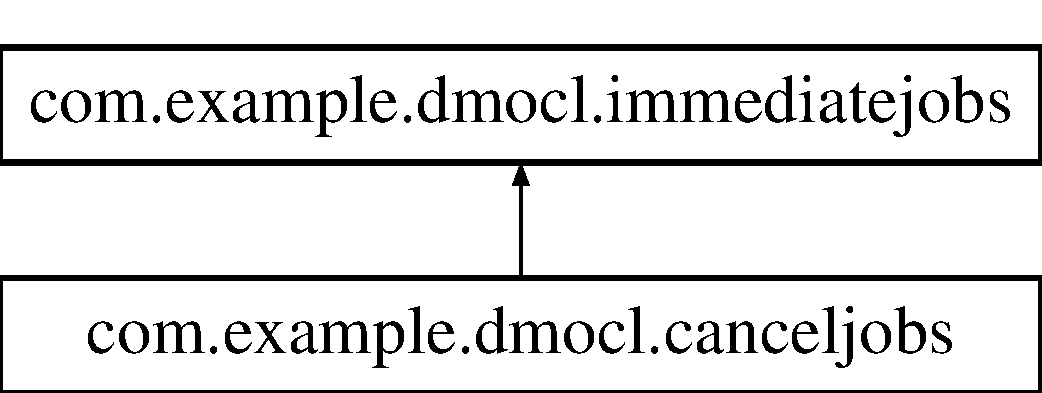
\includegraphics[height=2.000000cm]{classcom_1_1example_1_1dmocl_1_1canceljobs}
\end{center}
\end{figure}
\subsection*{Public Member Functions}
\begin{DoxyCompactItemize}
\item 
\mbox{\Hypertarget{classcom_1_1example_1_1dmocl_1_1canceljobs_a8a62b3a1ddf01cafbad4e709d9f7b1ea}\label{classcom_1_1example_1_1dmocl_1_1canceljobs_a8a62b3a1ddf01cafbad4e709d9f7b1ea}} 
{\bfseries canceljobs} (Handler result\+Handler, Executor executor, Context context, Text\+View jobinfo, Button startbutton)
\item 
\mbox{\Hypertarget{classcom_1_1example_1_1dmocl_1_1canceljobs_a1b44f0619185399f3b6a4d16f244f1ef}\label{classcom_1_1example_1_1dmocl_1_1canceljobs_a1b44f0619185399f3b6a4d16f244f1ef}} 
void {\bfseries startcanceljobs} (final Repository\+Callback$<$ jobschedresponse $>$ callback)
\end{DoxyCompactItemize}
\subsection*{Additional Inherited Members}


The documentation for this class was generated from the following file\+:\begin{DoxyCompactItemize}
\item 
/home/robert/\+Android\+Studio\+Projects/\+D\+M\+G\+P\+U/app/src/main/java/com/example/dmocl/canceljobs.\+java\end{DoxyCompactItemize}

\hypertarget{classcom_1_1example_1_1dmocl_1_1dataminingtask}{}\section{com.\+example.\+dmocl.\+dataminingtask Class Reference}
\label{classcom_1_1example_1_1dmocl_1_1dataminingtask}\index{com.\+example.\+dmocl.\+dataminingtask@{com.\+example.\+dmocl.\+dataminingtask}}
Inheritance diagram for com.\+example.\+dmocl.\+dataminingtask\+:\begin{figure}[H]
\begin{center}
\leavevmode
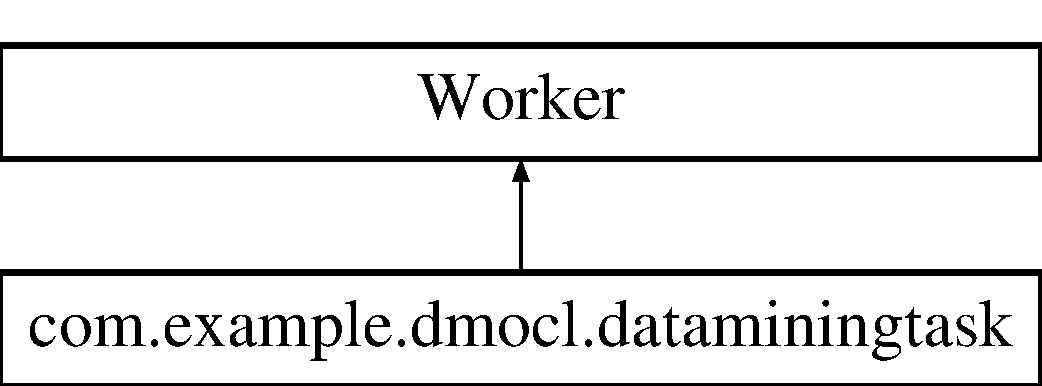
\includegraphics[height=2.000000cm]{classcom_1_1example_1_1dmocl_1_1dataminingtask}
\end{center}
\end{figure}
\subsection*{Public Member Functions}
\begin{DoxyCompactItemize}
\item 
\mbox{\Hypertarget{classcom_1_1example_1_1dmocl_1_1dataminingtask_adeb6d5795db66ea5aa050d442ad17959}\label{classcom_1_1example_1_1dmocl_1_1dataminingtask_adeb6d5795db66ea5aa050d442ad17959}} 
{\bfseries dataminingtask} ( @Non\+Null Context context, @Non\+Null Worker\+Parameters params)
\item 
\mbox{\Hypertarget{classcom_1_1example_1_1dmocl_1_1dataminingtask_a3ae06bc9b4443444284c6339c81252c4}\label{classcom_1_1example_1_1dmocl_1_1dataminingtask_a3ae06bc9b4443444284c6339c81252c4}} 
void {\bfseries on\+Stopped} ()
\item 
\mbox{\Hypertarget{classcom_1_1example_1_1dmocl_1_1dataminingtask_a39b5d15f90cab9ac6ce6f0d4d4797261}\label{classcom_1_1example_1_1dmocl_1_1dataminingtask_a39b5d15f90cab9ac6ce6f0d4d4797261}} 
Result {\bfseries do\+Work} ()
\end{DoxyCompactItemize}
\subsection*{Static Public Member Functions}
\begin{DoxyCompactItemize}
\item 
\mbox{\Hypertarget{classcom_1_1example_1_1dmocl_1_1dataminingtask_adbc8fcc905465705753dec21be6e9b9f}\label{classcom_1_1example_1_1dmocl_1_1dataminingtask_adbc8fcc905465705753dec21be6e9b9f}} 
static final String {\bfseries compileprogressoutput} (String fn, int z, int meth, int cores, int clusterno, short\mbox{[}$\,$\mbox{]} b, double wct)
\end{DoxyCompactItemize}
\subsection*{Static Public Attributes}
\begin{DoxyCompactItemize}
\item 
\mbox{\Hypertarget{classcom_1_1example_1_1dmocl_1_1dataminingtask_a27dbb6b1fb48631844198bfc5ceea344}\label{classcom_1_1example_1_1dmocl_1_1dataminingtask_a27dbb6b1fb48631844198bfc5ceea344}} 
static final String \mbox{[}$\,$\mbox{]} {\bfseries prependnames} = \{\char`\"{}Java\char`\"{}, \char`\"{}C\char`\"{}, \char`\"{}C+G\+PU\char`\"{}, \char`\"{}Java+Threads\char`\"{}, \char`\"{}C+Threads\char`\"{}\}
\end{DoxyCompactItemize}


The documentation for this class was generated from the following file\+:\begin{DoxyCompactItemize}
\item 
/home/robert/\+Android\+Studio\+Projects/\+D\+M\+G\+P\+U/app/src/main/java/com/example/dmocl/dataminingtask.\+java\end{DoxyCompactItemize}

\hypertarget{classcom_1_1example_1_1dmocl_1_1dbscan}{}\section{com.\+example.\+dmocl.\+dbscan Class Reference}
\label{classcom_1_1example_1_1dmocl_1_1dbscan}\index{com.\+example.\+dmocl.\+dbscan@{com.\+example.\+dmocl.\+dbscan}}
\subsection*{Classes}
\begin{DoxyCompactItemize}
\item 
class \mbox{\hyperlink{classcom_1_1example_1_1dmocl_1_1dbscan_1_1dbscan__thread1}{dbscan\+\_\+thread1}}
\item 
class \mbox{\hyperlink{classcom_1_1example_1_1dmocl_1_1dbscan_1_1dbscan__thread2}{dbscan\+\_\+thread2}}
\end{DoxyCompactItemize}
\subsection*{Static Public Member Functions}
\begin{DoxyCompactItemize}
\item 
static void \mbox{\hyperlink{classcom_1_1example_1_1dmocl_1_1dbscan_ac0a5610d6eb5ea04f0ac297bf2fc9465}{dbscanabort}} ()
\item 
static void \mbox{\hyperlink{classcom_1_1example_1_1dmocl_1_1dbscan_ae930532d5261bca83fff8c032c57460e}{dbscanresume}} ()
\item 
static native short \mbox{\hyperlink{classcom_1_1example_1_1dmocl_1_1dbscan_abdf678cb2bc1751842e632910df91ef2}{dbscan\+\_\+c}} (short\mbox{[}$\,$\mbox{]} b, float\mbox{[}$\,$\mbox{]} data, float eps, int kk, int features)
\item 
static native short \mbox{\hyperlink{classcom_1_1example_1_1dmocl_1_1dbscan_aff87d111fa96f0cefa39304a0ac02dff}{dbscan\+\_\+c\+\_\+gpu}} (short\mbox{[}$\,$\mbox{]} b, float\mbox{[}$\,$\mbox{]} data, float eps, int kk, int features, long\mbox{[}$\,$\mbox{]} e)
\item 
static native short \mbox{\hyperlink{classcom_1_1example_1_1dmocl_1_1dbscan_ae91b2a29faf3f05081f4163e27cd571a}{dbscan\+\_\+c\+\_\+phtreads}} (short\mbox{[}$\,$\mbox{]} b, float\mbox{[}$\,$\mbox{]} data, float eps, int kk, int features, int cores, long\mbox{[}$\,$\mbox{]} e)
\item 
static short \mbox{\hyperlink{classcom_1_1example_1_1dmocl_1_1dbscan_ae775963e50e6c01388ab1b1d7e604f57}{dbscan\+\_\+st}} (short\mbox{[}$\,$\mbox{]} b, float\mbox{[}$\,$\mbox{]} data, float eps, int kk, int features)
\item 
static short \mbox{\hyperlink{classcom_1_1example_1_1dmocl_1_1dbscan_a966ad9839294c6c28b7e43f974592345}{dbscan\+\_\+threads}} (short\mbox{[}$\,$\mbox{]} b, float\mbox{[}$\,$\mbox{]} data, float eps, int kk, int features, int cores, long\mbox{[}$\,$\mbox{]} ej)  throws Interrupted\+Exception 
\end{DoxyCompactItemize}
\subsection*{Static Package Functions}
\begin{DoxyCompactItemize}
\item 
\mbox{\hyperlink{classcom_1_1example_1_1dmocl_1_1dbscan_aa4b840bbdc7c3cfb22a09e3dc521a4e1}{\mbox{[}static initializer\mbox{]}}}
\end{DoxyCompactItemize}
\subsection*{Static Private Member Functions}
\begin{DoxyCompactItemize}
\item 
static native void \mbox{\hyperlink{classcom_1_1example_1_1dmocl_1_1dbscan_a9046c500df8074b1f4f57d4cb0c274a8}{dbscanabort\+\_\+c}} ()
\item 
static native void \mbox{\hyperlink{classcom_1_1example_1_1dmocl_1_1dbscan_af20fc5d6d88472f6af230198246c9fe5}{dbscanresume\+\_\+c}} ()
\item 
static short \mbox{\hyperlink{classcom_1_1example_1_1dmocl_1_1dbscan_af18896a5db63c0bbb718611405ceb89f}{expand\+Cluster\+\_\+st}} (int key, short clusternumber, short\mbox{[}$\,$\mbox{]} b, float\mbox{[}$\,$\mbox{]} data, float epseps, int kk, int features)
\item 
static short \mbox{\hyperlink{classcom_1_1example_1_1dmocl_1_1dbscan_a86a06d7cd50e45df5f69d8bbf484a966}{expand\+Cluster\+\_\+threads}} (int key, short clusternumber, short\mbox{[}$\,$\mbox{]} b, float\mbox{[}$\,$\mbox{]} data, float epseps, int kk, int features, int cores, \mbox{\hyperlink{classcom_1_1example_1_1dmocl_1_1dbscan_1_1dbscan__thread2}{dbscan\+\_\+thread2}}\mbox{[}$\,$\mbox{]} dbth2)  throws Interrupted\+Exception  
\end{DoxyCompactItemize}
\subsection*{Static Private Attributes}
\begin{DoxyCompactItemize}
\item 
static boolean \mbox{\hyperlink{classcom_1_1example_1_1dmocl_1_1dbscan_a614b6e11c265a9291ad5e7b2a81e3524}{doabort}} = false
\item 
static final Object \mbox{\hyperlink{classcom_1_1example_1_1dmocl_1_1dbscan_ad1fe5e758b8545a61ec38b2329ffc96d}{L\+O\+CK}} = new Object()
\item 
static final Reentrant\+Read\+Write\+Lock \mbox{\hyperlink{classcom_1_1example_1_1dmocl_1_1dbscan_a1a5afc44bad3ba73e68b4a298e42beba}{rrwl}} = new Reentrant\+Read\+Write\+Lock(true)
\end{DoxyCompactItemize}


\subsection{Member Function Documentation}
\mbox{\Hypertarget{classcom_1_1example_1_1dmocl_1_1dbscan_aa4b840bbdc7c3cfb22a09e3dc521a4e1}\label{classcom_1_1example_1_1dmocl_1_1dbscan_aa4b840bbdc7c3cfb22a09e3dc521a4e1}} 
\index{com\+::example\+::dmocl\+::dbscan@{com\+::example\+::dmocl\+::dbscan}!\mbox{[}static initializer\mbox{]}@{[static initializer]}}
\index{\mbox{[}static initializer\mbox{]}@{[static initializer]}!com\+::example\+::dmocl\+::dbscan@{com\+::example\+::dmocl\+::dbscan}}
\subsubsection{\texorpdfstring{[static initializer]()}{[static initializer]()}}
{\footnotesize\ttfamily com.\+example.\+dmocl.\+dbscan.\mbox{[}static initializer\mbox{]} (\begin{DoxyParamCaption}{ }\end{DoxyParamCaption})\hspace{0.3cm}{\ttfamily [inline]}, {\ttfamily [static]}, {\ttfamily [package]}}

\mbox{\Hypertarget{classcom_1_1example_1_1dmocl_1_1dbscan_abdf678cb2bc1751842e632910df91ef2}\label{classcom_1_1example_1_1dmocl_1_1dbscan_abdf678cb2bc1751842e632910df91ef2}} 
\index{com\+::example\+::dmocl\+::dbscan@{com\+::example\+::dmocl\+::dbscan}!dbscan\+\_\+c@{dbscan\+\_\+c}}
\index{dbscan\+\_\+c@{dbscan\+\_\+c}!com\+::example\+::dmocl\+::dbscan@{com\+::example\+::dmocl\+::dbscan}}
\subsubsection{\texorpdfstring{dbscan\+\_\+c()}{dbscan\_c()}}
{\footnotesize\ttfamily static native short com.\+example.\+dmocl.\+dbscan.\+dbscan\+\_\+c (\begin{DoxyParamCaption}\item[{short \mbox{[}$\,$\mbox{]}}]{b,  }\item[{float \mbox{[}$\,$\mbox{]}}]{data,  }\item[{float}]{eps,  }\item[{int}]{kk,  }\item[{int}]{features }\end{DoxyParamCaption})\hspace{0.3cm}{\ttfamily [static]}}

\mbox{\Hypertarget{classcom_1_1example_1_1dmocl_1_1dbscan_aff87d111fa96f0cefa39304a0ac02dff}\label{classcom_1_1example_1_1dmocl_1_1dbscan_aff87d111fa96f0cefa39304a0ac02dff}} 
\index{com\+::example\+::dmocl\+::dbscan@{com\+::example\+::dmocl\+::dbscan}!dbscan\+\_\+c\+\_\+gpu@{dbscan\+\_\+c\+\_\+gpu}}
\index{dbscan\+\_\+c\+\_\+gpu@{dbscan\+\_\+c\+\_\+gpu}!com\+::example\+::dmocl\+::dbscan@{com\+::example\+::dmocl\+::dbscan}}
\subsubsection{\texorpdfstring{dbscan\+\_\+c\+\_\+gpu()}{dbscan\_c\_gpu()}}
{\footnotesize\ttfamily static native short com.\+example.\+dmocl.\+dbscan.\+dbscan\+\_\+c\+\_\+gpu (\begin{DoxyParamCaption}\item[{short \mbox{[}$\,$\mbox{]}}]{b,  }\item[{float \mbox{[}$\,$\mbox{]}}]{data,  }\item[{float}]{eps,  }\item[{int}]{kk,  }\item[{int}]{features,  }\item[{long \mbox{[}$\,$\mbox{]}}]{e }\end{DoxyParamCaption})\hspace{0.3cm}{\ttfamily [static]}}

\mbox{\Hypertarget{classcom_1_1example_1_1dmocl_1_1dbscan_ae91b2a29faf3f05081f4163e27cd571a}\label{classcom_1_1example_1_1dmocl_1_1dbscan_ae91b2a29faf3f05081f4163e27cd571a}} 
\index{com\+::example\+::dmocl\+::dbscan@{com\+::example\+::dmocl\+::dbscan}!dbscan\+\_\+c\+\_\+phtreads@{dbscan\+\_\+c\+\_\+phtreads}}
\index{dbscan\+\_\+c\+\_\+phtreads@{dbscan\+\_\+c\+\_\+phtreads}!com\+::example\+::dmocl\+::dbscan@{com\+::example\+::dmocl\+::dbscan}}
\subsubsection{\texorpdfstring{dbscan\+\_\+c\+\_\+phtreads()}{dbscan\_c\_phtreads()}}
{\footnotesize\ttfamily static native short com.\+example.\+dmocl.\+dbscan.\+dbscan\+\_\+c\+\_\+phtreads (\begin{DoxyParamCaption}\item[{short \mbox{[}$\,$\mbox{]}}]{b,  }\item[{float \mbox{[}$\,$\mbox{]}}]{data,  }\item[{float}]{eps,  }\item[{int}]{kk,  }\item[{int}]{features,  }\item[{int}]{cores,  }\item[{long \mbox{[}$\,$\mbox{]}}]{e }\end{DoxyParamCaption})\hspace{0.3cm}{\ttfamily [static]}}

\mbox{\Hypertarget{classcom_1_1example_1_1dmocl_1_1dbscan_ae775963e50e6c01388ab1b1d7e604f57}\label{classcom_1_1example_1_1dmocl_1_1dbscan_ae775963e50e6c01388ab1b1d7e604f57}} 
\index{com\+::example\+::dmocl\+::dbscan@{com\+::example\+::dmocl\+::dbscan}!dbscan\+\_\+st@{dbscan\+\_\+st}}
\index{dbscan\+\_\+st@{dbscan\+\_\+st}!com\+::example\+::dmocl\+::dbscan@{com\+::example\+::dmocl\+::dbscan}}
\subsubsection{\texorpdfstring{dbscan\+\_\+st()}{dbscan\_st()}}
{\footnotesize\ttfamily static short com.\+example.\+dmocl.\+dbscan.\+dbscan\+\_\+st (\begin{DoxyParamCaption}\item[{short \mbox{[}$\,$\mbox{]}}]{b,  }\item[{float \mbox{[}$\,$\mbox{]}}]{data,  }\item[{float}]{eps,  }\item[{int}]{kk,  }\item[{int}]{features }\end{DoxyParamCaption})\hspace{0.3cm}{\ttfamily [inline]}, {\ttfamily [static]}}

\mbox{\Hypertarget{classcom_1_1example_1_1dmocl_1_1dbscan_a966ad9839294c6c28b7e43f974592345}\label{classcom_1_1example_1_1dmocl_1_1dbscan_a966ad9839294c6c28b7e43f974592345}} 
\index{com\+::example\+::dmocl\+::dbscan@{com\+::example\+::dmocl\+::dbscan}!dbscan\+\_\+threads@{dbscan\+\_\+threads}}
\index{dbscan\+\_\+threads@{dbscan\+\_\+threads}!com\+::example\+::dmocl\+::dbscan@{com\+::example\+::dmocl\+::dbscan}}
\subsubsection{\texorpdfstring{dbscan\+\_\+threads()}{dbscan\_threads()}}
{\footnotesize\ttfamily static short com.\+example.\+dmocl.\+dbscan.\+dbscan\+\_\+threads (\begin{DoxyParamCaption}\item[{short \mbox{[}$\,$\mbox{]}}]{b,  }\item[{float \mbox{[}$\,$\mbox{]}}]{data,  }\item[{float}]{eps,  }\item[{int}]{kk,  }\item[{int}]{features,  }\item[{int}]{cores,  }\item[{long \mbox{[}$\,$\mbox{]}}]{ej }\end{DoxyParamCaption}) throws Interrupted\+Exception\hspace{0.3cm}{\ttfamily [inline]}, {\ttfamily [static]}}

\mbox{\Hypertarget{classcom_1_1example_1_1dmocl_1_1dbscan_ac0a5610d6eb5ea04f0ac297bf2fc9465}\label{classcom_1_1example_1_1dmocl_1_1dbscan_ac0a5610d6eb5ea04f0ac297bf2fc9465}} 
\index{com\+::example\+::dmocl\+::dbscan@{com\+::example\+::dmocl\+::dbscan}!dbscanabort@{dbscanabort}}
\index{dbscanabort@{dbscanabort}!com\+::example\+::dmocl\+::dbscan@{com\+::example\+::dmocl\+::dbscan}}
\subsubsection{\texorpdfstring{dbscanabort()}{dbscanabort()}}
{\footnotesize\ttfamily static void com.\+example.\+dmocl.\+dbscan.\+dbscanabort (\begin{DoxyParamCaption}{ }\end{DoxyParamCaption})\hspace{0.3cm}{\ttfamily [inline]}, {\ttfamily [static]}}

\mbox{\Hypertarget{classcom_1_1example_1_1dmocl_1_1dbscan_a9046c500df8074b1f4f57d4cb0c274a8}\label{classcom_1_1example_1_1dmocl_1_1dbscan_a9046c500df8074b1f4f57d4cb0c274a8}} 
\index{com\+::example\+::dmocl\+::dbscan@{com\+::example\+::dmocl\+::dbscan}!dbscanabort\+\_\+c@{dbscanabort\+\_\+c}}
\index{dbscanabort\+\_\+c@{dbscanabort\+\_\+c}!com\+::example\+::dmocl\+::dbscan@{com\+::example\+::dmocl\+::dbscan}}
\subsubsection{\texorpdfstring{dbscanabort\+\_\+c()}{dbscanabort\_c()}}
{\footnotesize\ttfamily static native void com.\+example.\+dmocl.\+dbscan.\+dbscanabort\+\_\+c (\begin{DoxyParamCaption}{ }\end{DoxyParamCaption})\hspace{0.3cm}{\ttfamily [static]}, {\ttfamily [private]}}

\mbox{\Hypertarget{classcom_1_1example_1_1dmocl_1_1dbscan_ae930532d5261bca83fff8c032c57460e}\label{classcom_1_1example_1_1dmocl_1_1dbscan_ae930532d5261bca83fff8c032c57460e}} 
\index{com\+::example\+::dmocl\+::dbscan@{com\+::example\+::dmocl\+::dbscan}!dbscanresume@{dbscanresume}}
\index{dbscanresume@{dbscanresume}!com\+::example\+::dmocl\+::dbscan@{com\+::example\+::dmocl\+::dbscan}}
\subsubsection{\texorpdfstring{dbscanresume()}{dbscanresume()}}
{\footnotesize\ttfamily static void com.\+example.\+dmocl.\+dbscan.\+dbscanresume (\begin{DoxyParamCaption}{ }\end{DoxyParamCaption})\hspace{0.3cm}{\ttfamily [inline]}, {\ttfamily [static]}}

\mbox{\Hypertarget{classcom_1_1example_1_1dmocl_1_1dbscan_af20fc5d6d88472f6af230198246c9fe5}\label{classcom_1_1example_1_1dmocl_1_1dbscan_af20fc5d6d88472f6af230198246c9fe5}} 
\index{com\+::example\+::dmocl\+::dbscan@{com\+::example\+::dmocl\+::dbscan}!dbscanresume\+\_\+c@{dbscanresume\+\_\+c}}
\index{dbscanresume\+\_\+c@{dbscanresume\+\_\+c}!com\+::example\+::dmocl\+::dbscan@{com\+::example\+::dmocl\+::dbscan}}
\subsubsection{\texorpdfstring{dbscanresume\+\_\+c()}{dbscanresume\_c()}}
{\footnotesize\ttfamily static native void com.\+example.\+dmocl.\+dbscan.\+dbscanresume\+\_\+c (\begin{DoxyParamCaption}{ }\end{DoxyParamCaption})\hspace{0.3cm}{\ttfamily [static]}, {\ttfamily [private]}}

\mbox{\Hypertarget{classcom_1_1example_1_1dmocl_1_1dbscan_af18896a5db63c0bbb718611405ceb89f}\label{classcom_1_1example_1_1dmocl_1_1dbscan_af18896a5db63c0bbb718611405ceb89f}} 
\index{com\+::example\+::dmocl\+::dbscan@{com\+::example\+::dmocl\+::dbscan}!expand\+Cluster\+\_\+st@{expand\+Cluster\+\_\+st}}
\index{expand\+Cluster\+\_\+st@{expand\+Cluster\+\_\+st}!com\+::example\+::dmocl\+::dbscan@{com\+::example\+::dmocl\+::dbscan}}
\subsubsection{\texorpdfstring{expand\+Cluster\+\_\+st()}{expandCluster\_st()}}
{\footnotesize\ttfamily static short com.\+example.\+dmocl.\+dbscan.\+expand\+Cluster\+\_\+st (\begin{DoxyParamCaption}\item[{int}]{key,  }\item[{short}]{clusternumber,  }\item[{short \mbox{[}$\,$\mbox{]}}]{b,  }\item[{float \mbox{[}$\,$\mbox{]}}]{data,  }\item[{float}]{epseps,  }\item[{int}]{kk,  }\item[{int}]{features }\end{DoxyParamCaption})\hspace{0.3cm}{\ttfamily [inline]}, {\ttfamily [static]}, {\ttfamily [private]}}

\mbox{\Hypertarget{classcom_1_1example_1_1dmocl_1_1dbscan_a86a06d7cd50e45df5f69d8bbf484a966}\label{classcom_1_1example_1_1dmocl_1_1dbscan_a86a06d7cd50e45df5f69d8bbf484a966}} 
\index{com\+::example\+::dmocl\+::dbscan@{com\+::example\+::dmocl\+::dbscan}!expand\+Cluster\+\_\+threads@{expand\+Cluster\+\_\+threads}}
\index{expand\+Cluster\+\_\+threads@{expand\+Cluster\+\_\+threads}!com\+::example\+::dmocl\+::dbscan@{com\+::example\+::dmocl\+::dbscan}}
\subsubsection{\texorpdfstring{expand\+Cluster\+\_\+threads()}{expandCluster\_threads()}}
{\footnotesize\ttfamily static short com.\+example.\+dmocl.\+dbscan.\+expand\+Cluster\+\_\+threads (\begin{DoxyParamCaption}\item[{int}]{key,  }\item[{short}]{clusternumber,  }\item[{short \mbox{[}$\,$\mbox{]}}]{b,  }\item[{float \mbox{[}$\,$\mbox{]}}]{data,  }\item[{float}]{epseps,  }\item[{int}]{kk,  }\item[{int}]{features,  }\item[{int}]{cores,  }\item[{\mbox{\hyperlink{classcom_1_1example_1_1dmocl_1_1dbscan_1_1dbscan__thread2}{dbscan\+\_\+thread2}} \mbox{[}$\,$\mbox{]}}]{dbth2 }\end{DoxyParamCaption}) throws Interrupted\+Exception\hspace{0.3cm}{\ttfamily [inline]}, {\ttfamily [static]}, {\ttfamily [private]}}



\subsection{Member Data Documentation}
\mbox{\Hypertarget{classcom_1_1example_1_1dmocl_1_1dbscan_a614b6e11c265a9291ad5e7b2a81e3524}\label{classcom_1_1example_1_1dmocl_1_1dbscan_a614b6e11c265a9291ad5e7b2a81e3524}} 
\index{com\+::example\+::dmocl\+::dbscan@{com\+::example\+::dmocl\+::dbscan}!doabort@{doabort}}
\index{doabort@{doabort}!com\+::example\+::dmocl\+::dbscan@{com\+::example\+::dmocl\+::dbscan}}
\subsubsection{\texorpdfstring{doabort}{doabort}}
{\footnotesize\ttfamily boolean com.\+example.\+dmocl.\+dbscan.\+doabort = false\hspace{0.3cm}{\ttfamily [static]}, {\ttfamily [private]}}

\mbox{\Hypertarget{classcom_1_1example_1_1dmocl_1_1dbscan_ad1fe5e758b8545a61ec38b2329ffc96d}\label{classcom_1_1example_1_1dmocl_1_1dbscan_ad1fe5e758b8545a61ec38b2329ffc96d}} 
\index{com\+::example\+::dmocl\+::dbscan@{com\+::example\+::dmocl\+::dbscan}!L\+O\+CK@{L\+O\+CK}}
\index{L\+O\+CK@{L\+O\+CK}!com\+::example\+::dmocl\+::dbscan@{com\+::example\+::dmocl\+::dbscan}}
\subsubsection{\texorpdfstring{L\+O\+CK}{LOCK}}
{\footnotesize\ttfamily final Object com.\+example.\+dmocl.\+dbscan.\+L\+O\+CK = new Object()\hspace{0.3cm}{\ttfamily [static]}, {\ttfamily [private]}}

\mbox{\Hypertarget{classcom_1_1example_1_1dmocl_1_1dbscan_a1a5afc44bad3ba73e68b4a298e42beba}\label{classcom_1_1example_1_1dmocl_1_1dbscan_a1a5afc44bad3ba73e68b4a298e42beba}} 
\index{com\+::example\+::dmocl\+::dbscan@{com\+::example\+::dmocl\+::dbscan}!rrwl@{rrwl}}
\index{rrwl@{rrwl}!com\+::example\+::dmocl\+::dbscan@{com\+::example\+::dmocl\+::dbscan}}
\subsubsection{\texorpdfstring{rrwl}{rrwl}}
{\footnotesize\ttfamily final Reentrant\+Read\+Write\+Lock com.\+example.\+dmocl.\+dbscan.\+rrwl = new Reentrant\+Read\+Write\+Lock(true)\hspace{0.3cm}{\ttfamily [static]}, {\ttfamily [private]}}



The documentation for this class was generated from the following file\+:\begin{DoxyCompactItemize}
\item 
/home/robert/\+Android\+Studio\+Projects/\+D\+M\+G\+P\+U/app/src/main/java/com/example/dmocl/\mbox{\hyperlink{dbscan_8java}{dbscan.\+java}}\end{DoxyCompactItemize}

\hypertarget{structdbscan__pt}{}\section{dbscan\+\_\+pt Struct Reference}
\label{structdbscan__pt}\index{dbscan\+\_\+pt@{dbscan\+\_\+pt}}


Parameters for the D\+B\+S\+C\+AN thread.  


\subsection*{Public Attributes}
\begin{DoxyCompactItemize}
\item 
\mbox{\Hypertarget{structdbscan__pt_a5a42d9fe57034198ed5250f6f0ddb2cb}\label{structdbscan__pt_a5a42d9fe57034198ed5250f6f0ddb2cb}} 
unsigned short int \mbox{\hyperlink{structdbscan__pt_a5a42d9fe57034198ed5250f6f0ddb2cb}{status}}
\begin{DoxyCompactList}\small\item\em (const) status (needed only for setup and destruction) \end{DoxyCompactList}\item 
\mbox{\Hypertarget{structdbscan__pt_aaa1b99005b0207af9c85a6fc73368eb3}\label{structdbscan__pt_aaa1b99005b0207af9c85a6fc73368eb3}} 
int \mbox{\hyperlink{structdbscan__pt_aaa1b99005b0207af9c85a6fc73368eb3}{num}}
\begin{DoxyCompactList}\small\item\em (const) number of thread \end{DoxyCompactList}\item 
\mbox{\Hypertarget{structdbscan__pt_aab10762fb46be396c06f36c7b8f84f64}\label{structdbscan__pt_aab10762fb46be396c06f36c7b8f84f64}} 
unsigned short $\ast$ \mbox{\hyperlink{structdbscan__pt_aab10762fb46be396c06f36c7b8f84f64}{b}}
\begin{DoxyCompactList}\small\item\em (out) number of closest cluster center \end{DoxyCompactList}\item 
\mbox{\Hypertarget{structdbscan__pt_a1da0197a70e570bd30de1872fe60cd6b}\label{structdbscan__pt_a1da0197a70e570bd30de1872fe60cd6b}} 
float $\ast$ \mbox{\hyperlink{structdbscan__pt_a1da0197a70e570bd30de1872fe60cd6b}{data}}
\begin{DoxyCompactList}\small\item\em (const) input data \end{DoxyCompactList}\item 
\mbox{\Hypertarget{structdbscan__pt_ac172b388c85db693e07e954f7d29e681}\label{structdbscan__pt_ac172b388c85db693e07e954f7d29e681}} 
int \mbox{\hyperlink{structdbscan__pt_ac172b388c85db693e07e954f7d29e681}{blen}}
\begin{DoxyCompactList}\small\item\em (const) number of data items \end{DoxyCompactList}\item 
\mbox{\Hypertarget{structdbscan__pt_ae73ddeeaca04d08756b022115639d607}\label{structdbscan__pt_ae73ddeeaca04d08756b022115639d607}} 
float \mbox{\hyperlink{structdbscan__pt_ae73ddeeaca04d08756b022115639d607}{eps}}
\begin{DoxyCompactList}\small\item\em (const) radius \end{DoxyCompactList}\item 
\mbox{\Hypertarget{structdbscan__pt_a07b73afdc253e16524b7eae0f6ec26b4}\label{structdbscan__pt_a07b73afdc253e16524b7eae0f6ec26b4}} 
int \mbox{\hyperlink{structdbscan__pt_a07b73afdc253e16524b7eae0f6ec26b4}{kk}}
\begin{DoxyCompactList}\small\item\em (const) number of neighbours \end{DoxyCompactList}\item 
\mbox{\Hypertarget{structdbscan__pt_a22b641c18fac3731d31e9ded8c0c93eb}\label{structdbscan__pt_a22b641c18fac3731d31e9ded8c0c93eb}} 
int \mbox{\hyperlink{structdbscan__pt_a22b641c18fac3731d31e9ded8c0c93eb}{features}}
\begin{DoxyCompactList}\small\item\em (const) number of features per data item \end{DoxyCompactList}\item 
\mbox{\Hypertarget{structdbscan__pt_ab35e524b61208589ee28bbf4a79341ae}\label{structdbscan__pt_ab35e524b61208589ee28bbf4a79341ae}} 
int \mbox{\hyperlink{structdbscan__pt_ab35e524b61208589ee28bbf4a79341ae}{start}}
\begin{DoxyCompactList}\small\item\em (const) first data item \end{DoxyCompactList}\item 
\mbox{\Hypertarget{structdbscan__pt_a75fa5f27f7e41e5472087a847388daaf}\label{structdbscan__pt_a75fa5f27f7e41e5472087a847388daaf}} 
int \mbox{\hyperlink{structdbscan__pt_a75fa5f27f7e41e5472087a847388daaf}{len}}
\begin{DoxyCompactList}\small\item\em (const) last data item \end{DoxyCompactList}\item 
\mbox{\Hypertarget{structdbscan__pt_a2535cf2a4899d30b008b26dfa92bd44c}\label{structdbscan__pt_a2535cf2a4899d30b008b26dfa92bd44c}} 
pthread\+\_\+t \mbox{\hyperlink{structdbscan__pt_a2535cf2a4899d30b008b26dfa92bd44c}{thread1}}
\begin{DoxyCompactList}\small\item\em (const) holds the thread reference for the main loop thread \end{DoxyCompactList}\item 
\mbox{\Hypertarget{structdbscan__pt_a4c0ec8c2730f9a56a4b186692de79c47}\label{structdbscan__pt_a4c0ec8c2730f9a56a4b186692de79c47}} 
pthread\+\_\+t \mbox{\hyperlink{structdbscan__pt_a4c0ec8c2730f9a56a4b186692de79c47}{thread2}}
\begin{DoxyCompactList}\small\item\em (const) holds the thread reference for the cluster expand thread \end{DoxyCompactList}\item 
\mbox{\Hypertarget{structdbscan__pt_a716ce695e04d99f1e045fb9de1fb70f0}\label{structdbscan__pt_a716ce695e04d99f1e045fb9de1fb70f0}} 
sem\+\_\+t \mbox{\hyperlink{structdbscan__pt_a716ce695e04d99f1e045fb9de1fb70f0}{sem1}}
\begin{DoxyCompactList}\small\item\em (in) semaphore to wait on (main loop thread) \end{DoxyCompactList}\item 
\mbox{\Hypertarget{structdbscan__pt_af4a16a1139b3ee7e1dfcec9d415a8855}\label{structdbscan__pt_af4a16a1139b3ee7e1dfcec9d415a8855}} 
sem\+\_\+t \mbox{\hyperlink{structdbscan__pt_af4a16a1139b3ee7e1dfcec9d415a8855}{semret1}}
\begin{DoxyCompactList}\small\item\em (in) results ready sempahore (main loop thread) \end{DoxyCompactList}\item 
\mbox{\Hypertarget{structdbscan__pt_a5123f8b35d2933f40d493fe31dc062c5}\label{structdbscan__pt_a5123f8b35d2933f40d493fe31dc062c5}} 
sem\+\_\+t \mbox{\hyperlink{structdbscan__pt_a5123f8b35d2933f40d493fe31dc062c5}{sem2}}
\begin{DoxyCompactList}\small\item\em (in) semaphore to wait on (cluster expand thread) \end{DoxyCompactList}\item 
\mbox{\Hypertarget{structdbscan__pt_a229860660f580c96e3f00820dedc314f}\label{structdbscan__pt_a229860660f580c96e3f00820dedc314f}} 
sem\+\_\+t \mbox{\hyperlink{structdbscan__pt_a229860660f580c96e3f00820dedc314f}{semret2}}
\begin{DoxyCompactList}\small\item\em (in) results ready sempahore (cluster expand thread) \end{DoxyCompactList}\item 
\mbox{\Hypertarget{structdbscan__pt_aecd4ee021a0d72191163f578644813b4}\label{structdbscan__pt_aecd4ee021a0d72191163f578644813b4}} 
pthread\+\_\+mutex\+\_\+t \mbox{\hyperlink{structdbscan__pt_aecd4ee021a0d72191163f578644813b4}{M\+U\+T\+E\+X\+\_\+var1}}
\begin{DoxyCompactList}\small\item\em (in) lock the access to cmpto1 and itemcounter1 \end{DoxyCompactList}\item 
\mbox{\Hypertarget{structdbscan__pt_a50b8b3c19e72c2496e04595da3466fc6}\label{structdbscan__pt_a50b8b3c19e72c2496e04595da3466fc6}} 
volatile int \mbox{\hyperlink{structdbscan__pt_a50b8b3c19e72c2496e04595da3466fc6}{cmpto1}}
\begin{DoxyCompactList}\small\item\em (in) data item number to which to compare all others \end{DoxyCompactList}\item 
\mbox{\Hypertarget{structdbscan__pt_af71b0c6290be59f918f5fded65ca5aa0}\label{structdbscan__pt_af71b0c6290be59f918f5fded65ca5aa0}} 
volatile int \mbox{\hyperlink{structdbscan__pt_af71b0c6290be59f918f5fded65ca5aa0}{itemcounter1}}
\begin{DoxyCompactList}\small\item\em (out) number of itmes within radius \end{DoxyCompactList}\item 
\mbox{\Hypertarget{structdbscan__pt_ad60703d4e4e49b5676c314ffacdd3cc6}\label{structdbscan__pt_ad60703d4e4e49b5676c314ffacdd3cc6}} 
pthread\+\_\+mutex\+\_\+t \mbox{\hyperlink{structdbscan__pt_ad60703d4e4e49b5676c314ffacdd3cc6}{M\+U\+T\+E\+X\+\_\+var2}}
\begin{DoxyCompactList}\small\item\em (in) lock the access to cmpto2 and itemcounter2 \end{DoxyCompactList}\item 
\mbox{\Hypertarget{structdbscan__pt_ae90fa8f34589191559422b8d49321675}\label{structdbscan__pt_ae90fa8f34589191559422b8d49321675}} 
volatile int \mbox{\hyperlink{structdbscan__pt_ae90fa8f34589191559422b8d49321675}{cmpto2}}
\begin{DoxyCompactList}\small\item\em (in) data item number to which to compare all others \end{DoxyCompactList}\item 
\mbox{\Hypertarget{structdbscan__pt_a7282c5e97e591646a31c5762bf39bd3f}\label{structdbscan__pt_a7282c5e97e591646a31c5762bf39bd3f}} 
volatile int \mbox{\hyperlink{structdbscan__pt_a7282c5e97e591646a31c5762bf39bd3f}{itemcounter2}}
\begin{DoxyCompactList}\small\item\em (out) number of itmes within radius \end{DoxyCompactList}\item 
\mbox{\Hypertarget{structdbscan__pt_a9b4bcd3f61e899809341451edb698520}\label{structdbscan__pt_a9b4bcd3f61e899809341451edb698520}} 
pthread\+\_\+mutex\+\_\+t \mbox{\hyperlink{structdbscan__pt_a9b4bcd3f61e899809341451edb698520}{M\+U\+T\+E\+X\+\_\+fertig1}}
\begin{DoxyCompactList}\small\item\em (in) locks the access to fertig1 \end{DoxyCompactList}\item 
\mbox{\Hypertarget{structdbscan__pt_a8ce1ed79a8f30b769dbae5a3725d0bec}\label{structdbscan__pt_a8ce1ed79a8f30b769dbae5a3725d0bec}} 
volatile unsigned char \mbox{\hyperlink{structdbscan__pt_a8ce1ed79a8f30b769dbae5a3725d0bec}{fertig1}}
\begin{DoxyCompactList}\small\item\em (in) 1=terminate thread \end{DoxyCompactList}\item 
\mbox{\Hypertarget{structdbscan__pt_ade6e5b96f996f1d367a2595f7c237978}\label{structdbscan__pt_ade6e5b96f996f1d367a2595f7c237978}} 
pthread\+\_\+mutex\+\_\+t \mbox{\hyperlink{structdbscan__pt_ade6e5b96f996f1d367a2595f7c237978}{M\+U\+T\+E\+X\+\_\+fertig2}}
\begin{DoxyCompactList}\small\item\em (in) locks the access to fertig2 \end{DoxyCompactList}\item 
\mbox{\Hypertarget{structdbscan__pt_a6e02721843281f1f83499d2e7c3ffd32}\label{structdbscan__pt_a6e02721843281f1f83499d2e7c3ffd32}} 
volatile unsigned char \mbox{\hyperlink{structdbscan__pt_a6e02721843281f1f83499d2e7c3ffd32}{fertig2}}
\begin{DoxyCompactList}\small\item\em (in) 1=terminate thread \end{DoxyCompactList}\end{DoxyCompactItemize}


\subsection{Detailed Description}
Parameters for the D\+B\+S\+C\+AN thread. 

This struct holds the parameters for each D\+B\+S\+C\+AN thread. (in) means parameters that are N\+OT changed by the thread but may be changed by the method that submits the job. (const) means that the value is never changed after setup. (out) attributes are changed by the threads. This struct is used by two threads (dbscanthread1 and dbscanthread2). This struct may be used only by one of these two threads. The caller has to take care that this struct is not used by both threads at the same time. Nevertheless, all (const) attributes are readonly after initialization and may be read at any time. 

The documentation for this struct was generated from the following file\+:\begin{DoxyCompactItemize}
\item 
/home/robert/\+Android\+Studio\+Projects/\+D\+M\+G\+P\+U/app/src/\+C/source/\mbox{\hyperlink{dbscan__c_8c}{dbscan\+\_\+c.\+c}}\end{DoxyCompactItemize}

\hypertarget{classcom_1_1example_1_1dmocl_1_1immediatejobs}{}\section{com.\+example.\+dmocl.\+immediatejobs Class Reference}
\label{classcom_1_1example_1_1dmocl_1_1immediatejobs}\index{com.\+example.\+dmocl.\+immediatejobs@{com.\+example.\+dmocl.\+immediatejobs}}
Inheritance diagram for com.\+example.\+dmocl.\+immediatejobs\+:\begin{figure}[H]
\begin{center}
\leavevmode
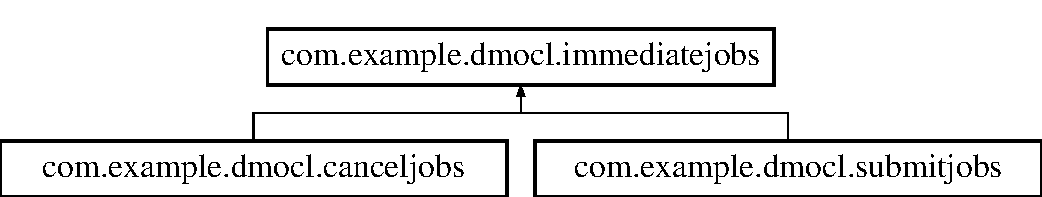
\includegraphics[height=2.000000cm]{classcom_1_1example_1_1dmocl_1_1immediatejobs}
\end{center}
\end{figure}
\subsection*{Classes}
\begin{DoxyCompactItemize}
\item 
class {\bfseries jobschedresponse}
\end{DoxyCompactItemize}
\subsection*{Protected Member Functions}
\begin{DoxyCompactItemize}
\item 
\mbox{\Hypertarget{classcom_1_1example_1_1dmocl_1_1immediatejobs_a5b2d3120e14b08e5712a4bce8728b60d}\label{classcom_1_1example_1_1dmocl_1_1immediatejobs_a5b2d3120e14b08e5712a4bce8728b60d}} 
void {\bfseries notify\+Result} (final Result$<$ canceljobs.\+jobschedresponse $>$ result, final Repository\+Callback$<$ canceljobs.\+jobschedresponse $>$ callback, final Handler result\+Handler)
\end{DoxyCompactItemize}


The documentation for this class was generated from the following file\+:\begin{DoxyCompactItemize}
\item 
/home/robert/\+Android\+Studio\+Projects/\+D\+M\+G\+P\+U/app/src/main/java/com/example/dmocl/immediatejobs.\+java\end{DoxyCompactItemize}

\hypertarget{classcom_1_1example_1_1dmocl_1_1kmeans}{}\section{com.\+example.\+dmocl.\+kmeans Class Reference}
\label{classcom_1_1example_1_1dmocl_1_1kmeans}\index{com.\+example.\+dmocl.\+kmeans@{com.\+example.\+dmocl.\+kmeans}}
\subsection*{Classes}
\begin{DoxyCompactItemize}
\item 
class \mbox{\hyperlink{classcom_1_1example_1_1dmocl_1_1kmeans_1_1kmeans__thread}{kmeans\+\_\+thread}}
\end{DoxyCompactItemize}
\subsection*{Static Public Member Functions}
\begin{DoxyCompactItemize}
\item 
static void \mbox{\hyperlink{classcom_1_1example_1_1dmocl_1_1kmeans_a8a721ea7f32bd548c7e1bd51eb7d18eb}{kmabort}} ()
\item 
static void \mbox{\hyperlink{classcom_1_1example_1_1dmocl_1_1kmeans_a5ba1945e6b7756886fd7a96babe493b7}{kmresume}} ()
\item 
static native short \mbox{\hyperlink{classcom_1_1example_1_1dmocl_1_1kmeans_a625b4b50289fb4b70df9f5e75d0171cc}{kmeans\+\_\+c}} (short\mbox{[}$\,$\mbox{]} b, float\mbox{[}$\,$\mbox{]} data, float eps, int cluno, int features)
\item 
static native short \mbox{\hyperlink{classcom_1_1example_1_1dmocl_1_1kmeans_afc49721ef1764e59e83082eb30e913b0}{kmeans\+\_\+c\+\_\+gpu}} (short\mbox{[}$\,$\mbox{]} b, float\mbox{[}$\,$\mbox{]} data, float eps, int cluno, int features, long\mbox{[}$\,$\mbox{]} e)
\item 
static native short \mbox{\hyperlink{classcom_1_1example_1_1dmocl_1_1kmeans_a87c0e078ffcfec39078fe9caf504af1e}{kmeans\+\_\+c\+\_\+phtreads}} (short\mbox{[}$\,$\mbox{]} b, float\mbox{[}$\,$\mbox{]} data, float eps, int cluno, int features, int cores, long\mbox{[}$\,$\mbox{]} e)
\item 
static short \mbox{\hyperlink{classcom_1_1example_1_1dmocl_1_1kmeans_a589995b7517109b01302666587ace215}{kmeans\+\_\+st}} (short\mbox{[}$\,$\mbox{]} b, float\mbox{[}$\,$\mbox{]} data, float eps, int cluno, int features)
\item 
static short \mbox{\hyperlink{classcom_1_1example_1_1dmocl_1_1kmeans_a9d1125246428c8ec0569608c88f1c7b7}{kmeans\+\_\+threads}} (short\mbox{[}$\,$\mbox{]} b, float\mbox{[}$\,$\mbox{]} data, float eps, int cluno, int features, int cores, long\mbox{[}$\,$\mbox{]} ej)  throws Interrupted\+Exception 
\end{DoxyCompactItemize}
\subsection*{Static Package Functions}
\begin{DoxyCompactItemize}
\item 
\mbox{\hyperlink{classcom_1_1example_1_1dmocl_1_1kmeans_a7fc606187903f49e8337e25de361bb32}{\mbox{[}static initializer\mbox{]}}}
\end{DoxyCompactItemize}
\subsection*{Static Package Attributes}
\begin{DoxyCompactItemize}
\item 
static final int \mbox{\hyperlink{classcom_1_1example_1_1dmocl_1_1kmeans_a1958a2698dea6fdc45c9a4986b48600f}{maxcycles}} = 100000
\end{DoxyCompactItemize}
\subsection*{Static Private Member Functions}
\begin{DoxyCompactItemize}
\item 
static native void \mbox{\hyperlink{classcom_1_1example_1_1dmocl_1_1kmeans_aaf412fa93eb8398f864218c5539342c8}{kmabort\+\_\+c}} ()
\item 
static native void \mbox{\hyperlink{classcom_1_1example_1_1dmocl_1_1kmeans_ab1cebe9efa8c81a62ccde2e6abf035c3}{kmresume\+\_\+c}} ()
\end{DoxyCompactItemize}
\subsection*{Static Private Attributes}
\begin{DoxyCompactItemize}
\item 
static boolean \mbox{\hyperlink{classcom_1_1example_1_1dmocl_1_1kmeans_ab7e7caf50f0c42b24eb806bf516c341e}{doabort}} = false
\item 
static final Object \mbox{\hyperlink{classcom_1_1example_1_1dmocl_1_1kmeans_ae84443fbb3a0c2eddc98d4cead831f5f}{L\+O\+C\+KA}} = new Object()
\item 
static final Reentrant\+Read\+Write\+Lock \mbox{\hyperlink{classcom_1_1example_1_1dmocl_1_1kmeans_a14088f43cd0164591d1fb9df377fc708}{rrwl}} = new Reentrant\+Read\+Write\+Lock(true)
\end{DoxyCompactItemize}


\subsection{Member Function Documentation}
\mbox{\Hypertarget{classcom_1_1example_1_1dmocl_1_1kmeans_a7fc606187903f49e8337e25de361bb32}\label{classcom_1_1example_1_1dmocl_1_1kmeans_a7fc606187903f49e8337e25de361bb32}} 
\index{com\+::example\+::dmocl\+::kmeans@{com\+::example\+::dmocl\+::kmeans}!\mbox{[}static initializer\mbox{]}@{[static initializer]}}
\index{\mbox{[}static initializer\mbox{]}@{[static initializer]}!com\+::example\+::dmocl\+::kmeans@{com\+::example\+::dmocl\+::kmeans}}
\subsubsection{\texorpdfstring{[static initializer]()}{[static initializer]()}}
{\footnotesize\ttfamily com.\+example.\+dmocl.\+kmeans.\mbox{[}static initializer\mbox{]} (\begin{DoxyParamCaption}{ }\end{DoxyParamCaption})\hspace{0.3cm}{\ttfamily [inline]}, {\ttfamily [static]}, {\ttfamily [package]}}

\mbox{\Hypertarget{classcom_1_1example_1_1dmocl_1_1kmeans_a8a721ea7f32bd548c7e1bd51eb7d18eb}\label{classcom_1_1example_1_1dmocl_1_1kmeans_a8a721ea7f32bd548c7e1bd51eb7d18eb}} 
\index{com\+::example\+::dmocl\+::kmeans@{com\+::example\+::dmocl\+::kmeans}!kmabort@{kmabort}}
\index{kmabort@{kmabort}!com\+::example\+::dmocl\+::kmeans@{com\+::example\+::dmocl\+::kmeans}}
\subsubsection{\texorpdfstring{kmabort()}{kmabort()}}
{\footnotesize\ttfamily static void com.\+example.\+dmocl.\+kmeans.\+kmabort (\begin{DoxyParamCaption}{ }\end{DoxyParamCaption})\hspace{0.3cm}{\ttfamily [inline]}, {\ttfamily [static]}}

\mbox{\Hypertarget{classcom_1_1example_1_1dmocl_1_1kmeans_aaf412fa93eb8398f864218c5539342c8}\label{classcom_1_1example_1_1dmocl_1_1kmeans_aaf412fa93eb8398f864218c5539342c8}} 
\index{com\+::example\+::dmocl\+::kmeans@{com\+::example\+::dmocl\+::kmeans}!kmabort\+\_\+c@{kmabort\+\_\+c}}
\index{kmabort\+\_\+c@{kmabort\+\_\+c}!com\+::example\+::dmocl\+::kmeans@{com\+::example\+::dmocl\+::kmeans}}
\subsubsection{\texorpdfstring{kmabort\+\_\+c()}{kmabort\_c()}}
{\footnotesize\ttfamily static native void com.\+example.\+dmocl.\+kmeans.\+kmabort\+\_\+c (\begin{DoxyParamCaption}{ }\end{DoxyParamCaption})\hspace{0.3cm}{\ttfamily [static]}, {\ttfamily [private]}}

\mbox{\Hypertarget{classcom_1_1example_1_1dmocl_1_1kmeans_a625b4b50289fb4b70df9f5e75d0171cc}\label{classcom_1_1example_1_1dmocl_1_1kmeans_a625b4b50289fb4b70df9f5e75d0171cc}} 
\index{com\+::example\+::dmocl\+::kmeans@{com\+::example\+::dmocl\+::kmeans}!kmeans\+\_\+c@{kmeans\+\_\+c}}
\index{kmeans\+\_\+c@{kmeans\+\_\+c}!com\+::example\+::dmocl\+::kmeans@{com\+::example\+::dmocl\+::kmeans}}
\subsubsection{\texorpdfstring{kmeans\+\_\+c()}{kmeans\_c()}}
{\footnotesize\ttfamily static native short com.\+example.\+dmocl.\+kmeans.\+kmeans\+\_\+c (\begin{DoxyParamCaption}\item[{short \mbox{[}$\,$\mbox{]}}]{b,  }\item[{float \mbox{[}$\,$\mbox{]}}]{data,  }\item[{float}]{eps,  }\item[{int}]{cluno,  }\item[{int}]{features }\end{DoxyParamCaption})\hspace{0.3cm}{\ttfamily [static]}}

\mbox{\Hypertarget{classcom_1_1example_1_1dmocl_1_1kmeans_afc49721ef1764e59e83082eb30e913b0}\label{classcom_1_1example_1_1dmocl_1_1kmeans_afc49721ef1764e59e83082eb30e913b0}} 
\index{com\+::example\+::dmocl\+::kmeans@{com\+::example\+::dmocl\+::kmeans}!kmeans\+\_\+c\+\_\+gpu@{kmeans\+\_\+c\+\_\+gpu}}
\index{kmeans\+\_\+c\+\_\+gpu@{kmeans\+\_\+c\+\_\+gpu}!com\+::example\+::dmocl\+::kmeans@{com\+::example\+::dmocl\+::kmeans}}
\subsubsection{\texorpdfstring{kmeans\+\_\+c\+\_\+gpu()}{kmeans\_c\_gpu()}}
{\footnotesize\ttfamily static native short com.\+example.\+dmocl.\+kmeans.\+kmeans\+\_\+c\+\_\+gpu (\begin{DoxyParamCaption}\item[{short \mbox{[}$\,$\mbox{]}}]{b,  }\item[{float \mbox{[}$\,$\mbox{]}}]{data,  }\item[{float}]{eps,  }\item[{int}]{cluno,  }\item[{int}]{features,  }\item[{long \mbox{[}$\,$\mbox{]}}]{e }\end{DoxyParamCaption})\hspace{0.3cm}{\ttfamily [static]}}

\mbox{\Hypertarget{classcom_1_1example_1_1dmocl_1_1kmeans_a87c0e078ffcfec39078fe9caf504af1e}\label{classcom_1_1example_1_1dmocl_1_1kmeans_a87c0e078ffcfec39078fe9caf504af1e}} 
\index{com\+::example\+::dmocl\+::kmeans@{com\+::example\+::dmocl\+::kmeans}!kmeans\+\_\+c\+\_\+phtreads@{kmeans\+\_\+c\+\_\+phtreads}}
\index{kmeans\+\_\+c\+\_\+phtreads@{kmeans\+\_\+c\+\_\+phtreads}!com\+::example\+::dmocl\+::kmeans@{com\+::example\+::dmocl\+::kmeans}}
\subsubsection{\texorpdfstring{kmeans\+\_\+c\+\_\+phtreads()}{kmeans\_c\_phtreads()}}
{\footnotesize\ttfamily static native short com.\+example.\+dmocl.\+kmeans.\+kmeans\+\_\+c\+\_\+phtreads (\begin{DoxyParamCaption}\item[{short \mbox{[}$\,$\mbox{]}}]{b,  }\item[{float \mbox{[}$\,$\mbox{]}}]{data,  }\item[{float}]{eps,  }\item[{int}]{cluno,  }\item[{int}]{features,  }\item[{int}]{cores,  }\item[{long \mbox{[}$\,$\mbox{]}}]{e }\end{DoxyParamCaption})\hspace{0.3cm}{\ttfamily [static]}}

\mbox{\Hypertarget{classcom_1_1example_1_1dmocl_1_1kmeans_a589995b7517109b01302666587ace215}\label{classcom_1_1example_1_1dmocl_1_1kmeans_a589995b7517109b01302666587ace215}} 
\index{com\+::example\+::dmocl\+::kmeans@{com\+::example\+::dmocl\+::kmeans}!kmeans\+\_\+st@{kmeans\+\_\+st}}
\index{kmeans\+\_\+st@{kmeans\+\_\+st}!com\+::example\+::dmocl\+::kmeans@{com\+::example\+::dmocl\+::kmeans}}
\subsubsection{\texorpdfstring{kmeans\+\_\+st()}{kmeans\_st()}}
{\footnotesize\ttfamily static short com.\+example.\+dmocl.\+kmeans.\+kmeans\+\_\+st (\begin{DoxyParamCaption}\item[{short \mbox{[}$\,$\mbox{]}}]{b,  }\item[{float \mbox{[}$\,$\mbox{]}}]{data,  }\item[{float}]{eps,  }\item[{int}]{cluno,  }\item[{int}]{features }\end{DoxyParamCaption})\hspace{0.3cm}{\ttfamily [inline]}, {\ttfamily [static]}}

\mbox{\Hypertarget{classcom_1_1example_1_1dmocl_1_1kmeans_a9d1125246428c8ec0569608c88f1c7b7}\label{classcom_1_1example_1_1dmocl_1_1kmeans_a9d1125246428c8ec0569608c88f1c7b7}} 
\index{com\+::example\+::dmocl\+::kmeans@{com\+::example\+::dmocl\+::kmeans}!kmeans\+\_\+threads@{kmeans\+\_\+threads}}
\index{kmeans\+\_\+threads@{kmeans\+\_\+threads}!com\+::example\+::dmocl\+::kmeans@{com\+::example\+::dmocl\+::kmeans}}
\subsubsection{\texorpdfstring{kmeans\+\_\+threads()}{kmeans\_threads()}}
{\footnotesize\ttfamily static short com.\+example.\+dmocl.\+kmeans.\+kmeans\+\_\+threads (\begin{DoxyParamCaption}\item[{short \mbox{[}$\,$\mbox{]}}]{b,  }\item[{float \mbox{[}$\,$\mbox{]}}]{data,  }\item[{float}]{eps,  }\item[{int}]{cluno,  }\item[{int}]{features,  }\item[{int}]{cores,  }\item[{long \mbox{[}$\,$\mbox{]}}]{ej }\end{DoxyParamCaption}) throws Interrupted\+Exception\hspace{0.3cm}{\ttfamily [inline]}, {\ttfamily [static]}}

\mbox{\Hypertarget{classcom_1_1example_1_1dmocl_1_1kmeans_a5ba1945e6b7756886fd7a96babe493b7}\label{classcom_1_1example_1_1dmocl_1_1kmeans_a5ba1945e6b7756886fd7a96babe493b7}} 
\index{com\+::example\+::dmocl\+::kmeans@{com\+::example\+::dmocl\+::kmeans}!kmresume@{kmresume}}
\index{kmresume@{kmresume}!com\+::example\+::dmocl\+::kmeans@{com\+::example\+::dmocl\+::kmeans}}
\subsubsection{\texorpdfstring{kmresume()}{kmresume()}}
{\footnotesize\ttfamily static void com.\+example.\+dmocl.\+kmeans.\+kmresume (\begin{DoxyParamCaption}{ }\end{DoxyParamCaption})\hspace{0.3cm}{\ttfamily [inline]}, {\ttfamily [static]}}

\mbox{\Hypertarget{classcom_1_1example_1_1dmocl_1_1kmeans_ab1cebe9efa8c81a62ccde2e6abf035c3}\label{classcom_1_1example_1_1dmocl_1_1kmeans_ab1cebe9efa8c81a62ccde2e6abf035c3}} 
\index{com\+::example\+::dmocl\+::kmeans@{com\+::example\+::dmocl\+::kmeans}!kmresume\+\_\+c@{kmresume\+\_\+c}}
\index{kmresume\+\_\+c@{kmresume\+\_\+c}!com\+::example\+::dmocl\+::kmeans@{com\+::example\+::dmocl\+::kmeans}}
\subsubsection{\texorpdfstring{kmresume\+\_\+c()}{kmresume\_c()}}
{\footnotesize\ttfamily static native void com.\+example.\+dmocl.\+kmeans.\+kmresume\+\_\+c (\begin{DoxyParamCaption}{ }\end{DoxyParamCaption})\hspace{0.3cm}{\ttfamily [static]}, {\ttfamily [private]}}



\subsection{Member Data Documentation}
\mbox{\Hypertarget{classcom_1_1example_1_1dmocl_1_1kmeans_ab7e7caf50f0c42b24eb806bf516c341e}\label{classcom_1_1example_1_1dmocl_1_1kmeans_ab7e7caf50f0c42b24eb806bf516c341e}} 
\index{com\+::example\+::dmocl\+::kmeans@{com\+::example\+::dmocl\+::kmeans}!doabort@{doabort}}
\index{doabort@{doabort}!com\+::example\+::dmocl\+::kmeans@{com\+::example\+::dmocl\+::kmeans}}
\subsubsection{\texorpdfstring{doabort}{doabort}}
{\footnotesize\ttfamily boolean com.\+example.\+dmocl.\+kmeans.\+doabort = false\hspace{0.3cm}{\ttfamily [static]}, {\ttfamily [private]}}

\mbox{\Hypertarget{classcom_1_1example_1_1dmocl_1_1kmeans_ae84443fbb3a0c2eddc98d4cead831f5f}\label{classcom_1_1example_1_1dmocl_1_1kmeans_ae84443fbb3a0c2eddc98d4cead831f5f}} 
\index{com\+::example\+::dmocl\+::kmeans@{com\+::example\+::dmocl\+::kmeans}!L\+O\+C\+KA@{L\+O\+C\+KA}}
\index{L\+O\+C\+KA@{L\+O\+C\+KA}!com\+::example\+::dmocl\+::kmeans@{com\+::example\+::dmocl\+::kmeans}}
\subsubsection{\texorpdfstring{L\+O\+C\+KA}{LOCKA}}
{\footnotesize\ttfamily final Object com.\+example.\+dmocl.\+kmeans.\+L\+O\+C\+KA = new Object()\hspace{0.3cm}{\ttfamily [static]}, {\ttfamily [private]}}

\mbox{\Hypertarget{classcom_1_1example_1_1dmocl_1_1kmeans_a1958a2698dea6fdc45c9a4986b48600f}\label{classcom_1_1example_1_1dmocl_1_1kmeans_a1958a2698dea6fdc45c9a4986b48600f}} 
\index{com\+::example\+::dmocl\+::kmeans@{com\+::example\+::dmocl\+::kmeans}!maxcycles@{maxcycles}}
\index{maxcycles@{maxcycles}!com\+::example\+::dmocl\+::kmeans@{com\+::example\+::dmocl\+::kmeans}}
\subsubsection{\texorpdfstring{maxcycles}{maxcycles}}
{\footnotesize\ttfamily final int com.\+example.\+dmocl.\+kmeans.\+maxcycles = 100000\hspace{0.3cm}{\ttfamily [static]}, {\ttfamily [package]}}

\mbox{\Hypertarget{classcom_1_1example_1_1dmocl_1_1kmeans_a14088f43cd0164591d1fb9df377fc708}\label{classcom_1_1example_1_1dmocl_1_1kmeans_a14088f43cd0164591d1fb9df377fc708}} 
\index{com\+::example\+::dmocl\+::kmeans@{com\+::example\+::dmocl\+::kmeans}!rrwl@{rrwl}}
\index{rrwl@{rrwl}!com\+::example\+::dmocl\+::kmeans@{com\+::example\+::dmocl\+::kmeans}}
\subsubsection{\texorpdfstring{rrwl}{rrwl}}
{\footnotesize\ttfamily final Reentrant\+Read\+Write\+Lock com.\+example.\+dmocl.\+kmeans.\+rrwl = new Reentrant\+Read\+Write\+Lock(true)\hspace{0.3cm}{\ttfamily [static]}, {\ttfamily [private]}}



The documentation for this class was generated from the following file\+:\begin{DoxyCompactItemize}
\item 
/home/robert/\+Android\+Studio\+Projects/\+D\+M\+G\+P\+U/app/src/main/java/com/example/dmocl/\mbox{\hyperlink{kmeans_8java}{kmeans.\+java}}\end{DoxyCompactItemize}

\hypertarget{structkmeans__pt}{}\section{kmeans\+\_\+pt Struct Reference}
\label{structkmeans__pt}\index{kmeans\+\_\+pt@{kmeans\+\_\+pt}}
\subsection*{Public Attributes}
\begin{DoxyCompactItemize}
\item 
\mbox{\Hypertarget{structkmeans__pt_adc9152bce7b95fd51d6185901169c52b}\label{structkmeans__pt_adc9152bce7b95fd51d6185901169c52b}} 
unsigned short int {\bfseries status}
\item 
\mbox{\Hypertarget{structkmeans__pt_a72c17b986e5cc7bbdcc92d59ef05e8f0}\label{structkmeans__pt_a72c17b986e5cc7bbdcc92d59ef05e8f0}} 
int {\bfseries num}
\item 
\mbox{\Hypertarget{structkmeans__pt_a00950024e02b55ade4be01f829f7f11d}\label{structkmeans__pt_a00950024e02b55ade4be01f829f7f11d}} 
unsigned short $\ast$ {\bfseries b}
\item 
\mbox{\Hypertarget{structkmeans__pt_a6efb6f48fc6294152d77552f183704da}\label{structkmeans__pt_a6efb6f48fc6294152d77552f183704da}} 
float $\ast$ {\bfseries data}
\item 
\mbox{\Hypertarget{structkmeans__pt_aca0bb922070f8b7dd1f0e82a4b8ca607}\label{structkmeans__pt_aca0bb922070f8b7dd1f0e82a4b8ca607}} 
volatile float $\ast$ {\bfseries clucent}
\item 
\mbox{\Hypertarget{structkmeans__pt_a4346d32e38a81feaf2799f25abf84a16}\label{structkmeans__pt_a4346d32e38a81feaf2799f25abf84a16}} 
int {\bfseries blen}
\item 
\mbox{\Hypertarget{structkmeans__pt_a987049eea35a32b1d1ba469f37b4a862}\label{structkmeans__pt_a987049eea35a32b1d1ba469f37b4a862}} 
int {\bfseries cluno}
\item 
\mbox{\Hypertarget{structkmeans__pt_a0b7e9c2f96d55642a579c66c916dfbac}\label{structkmeans__pt_a0b7e9c2f96d55642a579c66c916dfbac}} 
int {\bfseries features}
\item 
\mbox{\Hypertarget{structkmeans__pt_a7568dca47a635b63a775853ace1a231f}\label{structkmeans__pt_a7568dca47a635b63a775853ace1a231f}} 
int {\bfseries start}
\item 
\mbox{\Hypertarget{structkmeans__pt_af49609aa1989feab464cfc85a25c3ec4}\label{structkmeans__pt_af49609aa1989feab464cfc85a25c3ec4}} 
int {\bfseries len}
\item 
\mbox{\Hypertarget{structkmeans__pt_ad2580bc7fb5eac708522af779db2d54c}\label{structkmeans__pt_ad2580bc7fb5eac708522af779db2d54c}} 
volatile unsigned char {\bfseries fertig}
\item 
\mbox{\Hypertarget{structkmeans__pt_a2648d7c598e20fdf23e9d30f43b4b17c}\label{structkmeans__pt_a2648d7c598e20fdf23e9d30f43b4b17c}} 
pthread\+\_\+t {\bfseries thread}
\item 
\mbox{\Hypertarget{structkmeans__pt_af1c42a889c6180d899cb41066d2884c0}\label{structkmeans__pt_af1c42a889c6180d899cb41066d2884c0}} 
sem\+\_\+t {\bfseries sem}
\item 
\mbox{\Hypertarget{structkmeans__pt_aa959612fc7e6fa42798130bbf1c437a7}\label{structkmeans__pt_aa959612fc7e6fa42798130bbf1c437a7}} 
sem\+\_\+t {\bfseries semret}
\end{DoxyCompactItemize}


The documentation for this struct was generated from the following file\+:\begin{DoxyCompactItemize}
\item 
/home/robert/\+Android\+Studio\+Projects/\+D\+M\+G\+P\+U/app/src/\+C/source/kmeans\+\_\+c.\+c\end{DoxyCompactItemize}

\hypertarget{classcom_1_1example_1_1dmocl_1_1LinkToFile}{}\section{com.\+example.\+dmocl.\+Link\+To\+File Class Reference}
\label{classcom_1_1example_1_1dmocl_1_1LinkToFile}\index{com.\+example.\+dmocl.\+Link\+To\+File@{com.\+example.\+dmocl.\+Link\+To\+File}}


Save results and log to disk.  


\subsection*{Static Package Functions}
\begin{DoxyCompactItemize}
\item 
static synchronized void \mbox{\hyperlink{classcom_1_1example_1_1dmocl_1_1LinkToFile_a2ffa199a1de9e47644702409e25dd704}{D\+Mwrite\+To\+Fileheader}} (String fn)
\begin{DoxyCompactList}\small\item\em Writes the header line to the file. \end{DoxyCompactList}\item 
static synchronized void \mbox{\hyperlink{classcom_1_1example_1_1dmocl_1_1LinkToFile_a8cbd37ee89ecd01dcd55022c6ce74795}{D\+Mwrite\+To\+Fileheader}} (String fn, boolean append)
\begin{DoxyCompactList}\small\item\em Writes the header line to the file. \end{DoxyCompactList}\item 
static synchronized void \mbox{\hyperlink{classcom_1_1example_1_1dmocl_1_1LinkToFile_adb20b84275dde1b5b5808bfa80ec4969}{D\+Mwrite\+To\+File}} (String fn, String s)
\begin{DoxyCompactList}\small\item\em Writes a line to the result file. \end{DoxyCompactList}\item 
static synchronized void \mbox{\hyperlink{classcom_1_1example_1_1dmocl_1_1LinkToFile_a718e692d3583958f315ebe75c6569e74}{D\+Mwrite\+To\+Filefooter}} (String fn)
\begin{DoxyCompactList}\small\item\em Writes a footer line to the file. \end{DoxyCompactList}\item 
static synchronized void \mbox{\hyperlink{classcom_1_1example_1_1dmocl_1_1LinkToFile_a14393cd229c571ec80b236d1bd406e43}{D\+Mwrite\+To\+File}} (String fn, int cores, double\mbox{[}$\,$\mbox{]} wct, int size, int cluno, int features, int z)
\begin{DoxyCompactList}\small\item\em Writes results result file. \end{DoxyCompactList}\item 
static synchronized void \mbox{\hyperlink{classcom_1_1example_1_1dmocl_1_1LinkToFile_abc3a0a1a9269b671e24b8943480ae8aa}{log\+To\+File}} (String fn, String s, boolean append)
\begin{DoxyCompactList}\small\item\em Writes a line to the log file. \end{DoxyCompactList}\end{DoxyCompactItemize}


\subsection{Detailed Description}
Save results and log to disk. 

Saves the results and log information to the hard disk (S\+D-\/\+Card) of the device. 

\subsection{Member Function Documentation}
\mbox{\Hypertarget{classcom_1_1example_1_1dmocl_1_1LinkToFile_adb20b84275dde1b5b5808bfa80ec4969}\label{classcom_1_1example_1_1dmocl_1_1LinkToFile_adb20b84275dde1b5b5808bfa80ec4969}} 
\index{com\+::example\+::dmocl\+::\+Link\+To\+File@{com\+::example\+::dmocl\+::\+Link\+To\+File}!D\+Mwrite\+To\+File@{D\+Mwrite\+To\+File}}
\index{D\+Mwrite\+To\+File@{D\+Mwrite\+To\+File}!com\+::example\+::dmocl\+::\+Link\+To\+File@{com\+::example\+::dmocl\+::\+Link\+To\+File}}
\subsubsection{\texorpdfstring{D\+Mwrite\+To\+File()}{DMwriteToFile()}\hspace{0.1cm}{\footnotesize\ttfamily [1/2]}}
{\footnotesize\ttfamily static synchronized void com.\+example.\+dmocl.\+Link\+To\+File.\+D\+Mwrite\+To\+File (\begin{DoxyParamCaption}\item[{String}]{fn,  }\item[{String}]{s }\end{DoxyParamCaption})\hspace{0.3cm}{\ttfamily [inline]}, {\ttfamily [static]}, {\ttfamily [package]}}



Writes a line to the result file. 

Write a single line to the result file. 
\begin{DoxyParams}{Parameters}
{\em fn} & file name in which to write the header \\
\hline
{\em s} & the string to be written \\
\hline
\end{DoxyParams}
\begin{DoxyParagraph}{Multithreading\+:}
fully (methods are synchronized) 
\end{DoxyParagraph}
\mbox{\Hypertarget{classcom_1_1example_1_1dmocl_1_1LinkToFile_a14393cd229c571ec80b236d1bd406e43}\label{classcom_1_1example_1_1dmocl_1_1LinkToFile_a14393cd229c571ec80b236d1bd406e43}} 
\index{com\+::example\+::dmocl\+::\+Link\+To\+File@{com\+::example\+::dmocl\+::\+Link\+To\+File}!D\+Mwrite\+To\+File@{D\+Mwrite\+To\+File}}
\index{D\+Mwrite\+To\+File@{D\+Mwrite\+To\+File}!com\+::example\+::dmocl\+::\+Link\+To\+File@{com\+::example\+::dmocl\+::\+Link\+To\+File}}
\subsubsection{\texorpdfstring{D\+Mwrite\+To\+File()}{DMwriteToFile()}\hspace{0.1cm}{\footnotesize\ttfamily [2/2]}}
{\footnotesize\ttfamily static synchronized void com.\+example.\+dmocl.\+Link\+To\+File.\+D\+Mwrite\+To\+File (\begin{DoxyParamCaption}\item[{String}]{fn,  }\item[{int}]{cores,  }\item[{double \mbox{[}$\,$\mbox{]}}]{wct,  }\item[{int}]{size,  }\item[{int}]{cluno,  }\item[{int}]{features,  }\item[{int}]{z }\end{DoxyParamCaption})\hspace{0.3cm}{\ttfamily [inline]}, {\ttfamily [static]}, {\ttfamily [package]}}



Writes results result file. 

Write a single line of results to the result file. 
\begin{DoxyParams}{Parameters}
{\em fn} & file name in which to write the header \\
\hline
{\em cores} & number of cores used \\
\hline
{\em wct} & array with the wall clock times used \\
\hline
{\em size} & size of the cluster \\
\hline
{\em cluno} & number of clusters used \\
\hline
{\em features} & number of features used \\
\hline
{\em z} & 0=D\+B\+S\+C\+AN results equal, 1=D\+B\+S\+C\+AN results different \\
\hline
\end{DoxyParams}
\begin{DoxyParagraph}{Multithreading\+:}
fully (methods are synchronized) 
\end{DoxyParagraph}
\mbox{\Hypertarget{classcom_1_1example_1_1dmocl_1_1LinkToFile_a718e692d3583958f315ebe75c6569e74}\label{classcom_1_1example_1_1dmocl_1_1LinkToFile_a718e692d3583958f315ebe75c6569e74}} 
\index{com\+::example\+::dmocl\+::\+Link\+To\+File@{com\+::example\+::dmocl\+::\+Link\+To\+File}!D\+Mwrite\+To\+Filefooter@{D\+Mwrite\+To\+Filefooter}}
\index{D\+Mwrite\+To\+Filefooter@{D\+Mwrite\+To\+Filefooter}!com\+::example\+::dmocl\+::\+Link\+To\+File@{com\+::example\+::dmocl\+::\+Link\+To\+File}}
\subsubsection{\texorpdfstring{D\+Mwrite\+To\+Filefooter()}{DMwriteToFilefooter()}}
{\footnotesize\ttfamily static synchronized void com.\+example.\+dmocl.\+Link\+To\+File.\+D\+Mwrite\+To\+Filefooter (\begin{DoxyParamCaption}\item[{String}]{fn }\end{DoxyParamCaption})\hspace{0.3cm}{\ttfamily [inline]}, {\ttfamily [static]}, {\ttfamily [package]}}



Writes a footer line to the file. 

Write a footer line to the result file. 
\begin{DoxyParams}{Parameters}
{\em fn} & file name in which to write the header \\
\hline
\end{DoxyParams}
\begin{DoxyParagraph}{Multithreading\+:}
fully (methods are synchronized) 
\end{DoxyParagraph}
\mbox{\Hypertarget{classcom_1_1example_1_1dmocl_1_1LinkToFile_a2ffa199a1de9e47644702409e25dd704}\label{classcom_1_1example_1_1dmocl_1_1LinkToFile_a2ffa199a1de9e47644702409e25dd704}} 
\index{com\+::example\+::dmocl\+::\+Link\+To\+File@{com\+::example\+::dmocl\+::\+Link\+To\+File}!D\+Mwrite\+To\+Fileheader@{D\+Mwrite\+To\+Fileheader}}
\index{D\+Mwrite\+To\+Fileheader@{D\+Mwrite\+To\+Fileheader}!com\+::example\+::dmocl\+::\+Link\+To\+File@{com\+::example\+::dmocl\+::\+Link\+To\+File}}
\subsubsection{\texorpdfstring{D\+Mwrite\+To\+Fileheader()}{DMwriteToFileheader()}\hspace{0.1cm}{\footnotesize\ttfamily [1/2]}}
{\footnotesize\ttfamily static synchronized void com.\+example.\+dmocl.\+Link\+To\+File.\+D\+Mwrite\+To\+Fileheader (\begin{DoxyParamCaption}\item[{String}]{fn }\end{DoxyParamCaption})\hspace{0.3cm}{\ttfamily [inline]}, {\ttfamily [static]}, {\ttfamily [package]}}



Writes the header line to the file. 

Write the header line to the result file. Existing results are overwritten. 
\begin{DoxyParams}{Parameters}
{\em fn} & file name in which to write the header \\
\hline
\end{DoxyParams}
\begin{DoxyParagraph}{Multithreading\+:}
fully (methods are synchronized) 
\end{DoxyParagraph}
\mbox{\Hypertarget{classcom_1_1example_1_1dmocl_1_1LinkToFile_a8cbd37ee89ecd01dcd55022c6ce74795}\label{classcom_1_1example_1_1dmocl_1_1LinkToFile_a8cbd37ee89ecd01dcd55022c6ce74795}} 
\index{com\+::example\+::dmocl\+::\+Link\+To\+File@{com\+::example\+::dmocl\+::\+Link\+To\+File}!D\+Mwrite\+To\+Fileheader@{D\+Mwrite\+To\+Fileheader}}
\index{D\+Mwrite\+To\+Fileheader@{D\+Mwrite\+To\+Fileheader}!com\+::example\+::dmocl\+::\+Link\+To\+File@{com\+::example\+::dmocl\+::\+Link\+To\+File}}
\subsubsection{\texorpdfstring{D\+Mwrite\+To\+Fileheader()}{DMwriteToFileheader()}\hspace{0.1cm}{\footnotesize\ttfamily [2/2]}}
{\footnotesize\ttfamily static synchronized void com.\+example.\+dmocl.\+Link\+To\+File.\+D\+Mwrite\+To\+Fileheader (\begin{DoxyParamCaption}\item[{String}]{fn,  }\item[{boolean}]{append }\end{DoxyParamCaption})\hspace{0.3cm}{\ttfamily [inline]}, {\ttfamily [static]}, {\ttfamily [package]}}



Writes the header line to the file. 

Write the header line to the result file. The header line may be appended to existing results. 
\begin{DoxyParams}{Parameters}
{\em fn} & file name in which to write the header \\
\hline
{\em append} & true=append, false=overwrite \\
\hline
\end{DoxyParams}
\begin{DoxyParagraph}{Multithreading\+:}
fully (methods are synchronized) 
\end{DoxyParagraph}
\mbox{\Hypertarget{classcom_1_1example_1_1dmocl_1_1LinkToFile_abc3a0a1a9269b671e24b8943480ae8aa}\label{classcom_1_1example_1_1dmocl_1_1LinkToFile_abc3a0a1a9269b671e24b8943480ae8aa}} 
\index{com\+::example\+::dmocl\+::\+Link\+To\+File@{com\+::example\+::dmocl\+::\+Link\+To\+File}!log\+To\+File@{log\+To\+File}}
\index{log\+To\+File@{log\+To\+File}!com\+::example\+::dmocl\+::\+Link\+To\+File@{com\+::example\+::dmocl\+::\+Link\+To\+File}}
\subsubsection{\texorpdfstring{log\+To\+File()}{logToFile()}}
{\footnotesize\ttfamily static synchronized void com.\+example.\+dmocl.\+Link\+To\+File.\+log\+To\+File (\begin{DoxyParamCaption}\item[{String}]{fn,  }\item[{String}]{s,  }\item[{boolean}]{append }\end{DoxyParamCaption})\hspace{0.3cm}{\ttfamily [inline]}, {\ttfamily [static]}, {\ttfamily [package]}}



Writes a line to the log file. 

Write a single line to the log file. 
\begin{DoxyParams}{Parameters}
{\em fn} & file name in which to write the header \\
\hline
{\em s} & string to write \\
\hline
{\em append} & true=append to log file, false=overwrite log file \\
\hline
\end{DoxyParams}
\begin{DoxyParagraph}{Multithreading\+:}
fully (methods are synchronized) 
\end{DoxyParagraph}


The documentation for this class was generated from the following file\+:\begin{DoxyCompactItemize}
\item 
/home/robert/\+Android\+Studio\+Projects/\+D\+M\+G\+P\+U/app/src/main/java/com/example/dmocl/\mbox{\hyperlink{LinkToFile_8java}{Link\+To\+File.\+java}}\end{DoxyCompactItemize}

\hypertarget{classcom_1_1example_1_1dmocl_1_1MainActivity}{}\section{com.\+example.\+dmocl.\+Main\+Activity Class Reference}
\label{classcom_1_1example_1_1dmocl_1_1MainActivity}\index{com.\+example.\+dmocl.\+Main\+Activity@{com.\+example.\+dmocl.\+Main\+Activity}}
Inheritance diagram for com.\+example.\+dmocl.\+Main\+Activity\+:\begin{figure}[H]
\begin{center}
\leavevmode
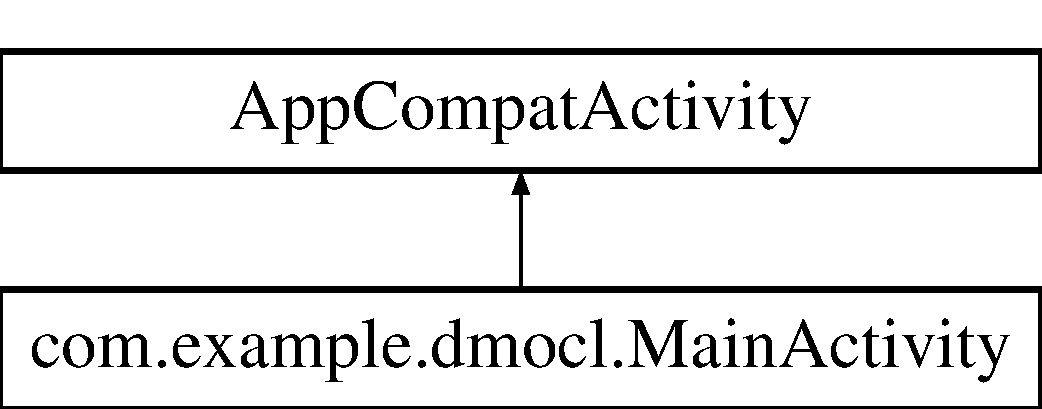
\includegraphics[height=2.000000cm]{classcom_1_1example_1_1dmocl_1_1MainActivity}
\end{center}
\end{figure}
\subsection*{Classes}
\begin{DoxyCompactItemize}
\item 
class \mbox{\hyperlink{classcom_1_1example_1_1dmocl_1_1MainActivity_1_1WorkManagerNoInformationException}{Work\+Manager\+No\+Information\+Exception}}
\end{DoxyCompactItemize}
\subsection*{Protected Member Functions}
\begin{DoxyCompactItemize}
\item 
synchronized boolean \mbox{\hyperlink{classcom_1_1example_1_1dmocl_1_1MainActivity_a26973c08d4b74dcce01e294077211c2f}{try\+Load\+G\+PU}} (String gpupath)
\item 
void \mbox{\hyperlink{classcom_1_1example_1_1dmocl_1_1MainActivity_a59609da2fb62ee158da1d4efc6d26f63}{on\+Resume}} ()
\item 
void \mbox{\hyperlink{classcom_1_1example_1_1dmocl_1_1MainActivity_a10f895ac3f6343c7b6c3b946ceadbf32}{on\+Create}} (Bundle saved\+Instance\+State)
\item 
void \mbox{\hyperlink{classcom_1_1example_1_1dmocl_1_1MainActivity_a0ba841e058a14398a5a6766e0618bd59}{on\+Destroy}} ()
\end{DoxyCompactItemize}
\subsection*{Package Attributes}
\begin{DoxyCompactItemize}
\item 
String \mbox{\hyperlink{classcom_1_1example_1_1dmocl_1_1MainActivity_aade6435b69c9fe19247a61b67a8bc6c4}{G\+P\+Upath}} = \char`\"{}\char`\"{}
\item 
Atomic\+Boolean \mbox{\hyperlink{classcom_1_1example_1_1dmocl_1_1MainActivity_a202e63994768ec6b848cc5ea8d0bc7fa}{G\+P\+Ufound}} = new Atomic\+Boolean(false)
\item 
Executor\+Service \mbox{\hyperlink{classcom_1_1example_1_1dmocl_1_1MainActivity_a3cb13ff3b6a5bb8274a82b5e5531babc}{executor\+Service}} = Executors.\+new\+Single\+Thread\+Executor()
\item 
Handler \mbox{\hyperlink{classcom_1_1example_1_1dmocl_1_1MainActivity_a1ee4246708662ea604b9c5485f37daa6}{main\+Thread\+Handler}} = Handler\+Compat.\+create\+Async(Looper.\+get\+Main\+Looper())
\end{DoxyCompactItemize}
\subsection*{Private Member Functions}
\begin{DoxyCompactItemize}
\item 
void \mbox{\hyperlink{classcom_1_1example_1_1dmocl_1_1MainActivity_a68c83a580a869fcaed554bee7fccfef4}{update\+Live\+Info}} (List$<$ Work\+Info $>$ statuses, Text\+View jobinfo, Button startbutton)  throws Work\+Manager\+No\+Information\+Exception 
\end{DoxyCompactItemize}
\subsection*{Private Attributes}
\begin{DoxyCompactItemize}
\item 
final Object \mbox{\hyperlink{classcom_1_1example_1_1dmocl_1_1MainActivity_aab1bd415da3d75e0223a77caa941333d}{syncobj}} = new Object()
\item 
final \mbox{\hyperlink{classcom_1_1example_1_1dmocl_1_1oclwrap}{oclwrap}} \mbox{\hyperlink{classcom_1_1example_1_1dmocl_1_1MainActivity_ac96a1197ded8a7cf0cb4ea39d37af6a6}{owrp}} = \mbox{\hyperlink{classcom_1_1example_1_1dmocl_1_1oclwrap_a8c8c9a75d3d834cb71725d92ddeb4af7}{oclwrap.\+get\+Ocl\+Wrapper}}()
\end{DoxyCompactItemize}


\subsection{Member Function Documentation}
\mbox{\Hypertarget{classcom_1_1example_1_1dmocl_1_1MainActivity_a10f895ac3f6343c7b6c3b946ceadbf32}\label{classcom_1_1example_1_1dmocl_1_1MainActivity_a10f895ac3f6343c7b6c3b946ceadbf32}} 
\index{com\+::example\+::dmocl\+::\+Main\+Activity@{com\+::example\+::dmocl\+::\+Main\+Activity}!on\+Create@{on\+Create}}
\index{on\+Create@{on\+Create}!com\+::example\+::dmocl\+::\+Main\+Activity@{com\+::example\+::dmocl\+::\+Main\+Activity}}
\subsubsection{\texorpdfstring{on\+Create()}{onCreate()}}
{\footnotesize\ttfamily void com.\+example.\+dmocl.\+Main\+Activity.\+on\+Create (\begin{DoxyParamCaption}\item[{Bundle}]{saved\+Instance\+State }\end{DoxyParamCaption})\hspace{0.3cm}{\ttfamily [inline]}, {\ttfamily [protected]}}

\mbox{\Hypertarget{classcom_1_1example_1_1dmocl_1_1MainActivity_a0ba841e058a14398a5a6766e0618bd59}\label{classcom_1_1example_1_1dmocl_1_1MainActivity_a0ba841e058a14398a5a6766e0618bd59}} 
\index{com\+::example\+::dmocl\+::\+Main\+Activity@{com\+::example\+::dmocl\+::\+Main\+Activity}!on\+Destroy@{on\+Destroy}}
\index{on\+Destroy@{on\+Destroy}!com\+::example\+::dmocl\+::\+Main\+Activity@{com\+::example\+::dmocl\+::\+Main\+Activity}}
\subsubsection{\texorpdfstring{on\+Destroy()}{onDestroy()}}
{\footnotesize\ttfamily void com.\+example.\+dmocl.\+Main\+Activity.\+on\+Destroy (\begin{DoxyParamCaption}{ }\end{DoxyParamCaption})\hspace{0.3cm}{\ttfamily [inline]}, {\ttfamily [protected]}}

\mbox{\Hypertarget{classcom_1_1example_1_1dmocl_1_1MainActivity_a59609da2fb62ee158da1d4efc6d26f63}\label{classcom_1_1example_1_1dmocl_1_1MainActivity_a59609da2fb62ee158da1d4efc6d26f63}} 
\index{com\+::example\+::dmocl\+::\+Main\+Activity@{com\+::example\+::dmocl\+::\+Main\+Activity}!on\+Resume@{on\+Resume}}
\index{on\+Resume@{on\+Resume}!com\+::example\+::dmocl\+::\+Main\+Activity@{com\+::example\+::dmocl\+::\+Main\+Activity}}
\subsubsection{\texorpdfstring{on\+Resume()}{onResume()}}
{\footnotesize\ttfamily void com.\+example.\+dmocl.\+Main\+Activity.\+on\+Resume (\begin{DoxyParamCaption}{ }\end{DoxyParamCaption})\hspace{0.3cm}{\ttfamily [inline]}, {\ttfamily [protected]}}

\mbox{\Hypertarget{classcom_1_1example_1_1dmocl_1_1MainActivity_a26973c08d4b74dcce01e294077211c2f}\label{classcom_1_1example_1_1dmocl_1_1MainActivity_a26973c08d4b74dcce01e294077211c2f}} 
\index{com\+::example\+::dmocl\+::\+Main\+Activity@{com\+::example\+::dmocl\+::\+Main\+Activity}!try\+Load\+G\+PU@{try\+Load\+G\+PU}}
\index{try\+Load\+G\+PU@{try\+Load\+G\+PU}!com\+::example\+::dmocl\+::\+Main\+Activity@{com\+::example\+::dmocl\+::\+Main\+Activity}}
\subsubsection{\texorpdfstring{try\+Load\+G\+P\+U()}{tryLoadGPU()}}
{\footnotesize\ttfamily synchronized boolean com.\+example.\+dmocl.\+Main\+Activity.\+try\+Load\+G\+PU (\begin{DoxyParamCaption}\item[{String}]{gpupath }\end{DoxyParamCaption})\hspace{0.3cm}{\ttfamily [inline]}, {\ttfamily [protected]}}

\mbox{\Hypertarget{classcom_1_1example_1_1dmocl_1_1MainActivity_a68c83a580a869fcaed554bee7fccfef4}\label{classcom_1_1example_1_1dmocl_1_1MainActivity_a68c83a580a869fcaed554bee7fccfef4}} 
\index{com\+::example\+::dmocl\+::\+Main\+Activity@{com\+::example\+::dmocl\+::\+Main\+Activity}!update\+Live\+Info@{update\+Live\+Info}}
\index{update\+Live\+Info@{update\+Live\+Info}!com\+::example\+::dmocl\+::\+Main\+Activity@{com\+::example\+::dmocl\+::\+Main\+Activity}}
\subsubsection{\texorpdfstring{update\+Live\+Info()}{updateLiveInfo()}}
{\footnotesize\ttfamily void com.\+example.\+dmocl.\+Main\+Activity.\+update\+Live\+Info (\begin{DoxyParamCaption}\item[{List$<$ Work\+Info $>$}]{statuses,  }\item[{Text\+View}]{jobinfo,  }\item[{Button}]{startbutton }\end{DoxyParamCaption}) throws \mbox{\hyperlink{classcom_1_1example_1_1dmocl_1_1MainActivity_1_1WorkManagerNoInformationException}{Work\+Manager\+No\+Information\+Exception}}\hspace{0.3cm}{\ttfamily [inline]}, {\ttfamily [private]}}



\subsection{Member Data Documentation}
\mbox{\Hypertarget{classcom_1_1example_1_1dmocl_1_1MainActivity_a3cb13ff3b6a5bb8274a82b5e5531babc}\label{classcom_1_1example_1_1dmocl_1_1MainActivity_a3cb13ff3b6a5bb8274a82b5e5531babc}} 
\index{com\+::example\+::dmocl\+::\+Main\+Activity@{com\+::example\+::dmocl\+::\+Main\+Activity}!executor\+Service@{executor\+Service}}
\index{executor\+Service@{executor\+Service}!com\+::example\+::dmocl\+::\+Main\+Activity@{com\+::example\+::dmocl\+::\+Main\+Activity}}
\subsubsection{\texorpdfstring{executor\+Service}{executorService}}
{\footnotesize\ttfamily Executor\+Service com.\+example.\+dmocl.\+Main\+Activity.\+executor\+Service = Executors.\+new\+Single\+Thread\+Executor()\hspace{0.3cm}{\ttfamily [package]}}

\mbox{\Hypertarget{classcom_1_1example_1_1dmocl_1_1MainActivity_a202e63994768ec6b848cc5ea8d0bc7fa}\label{classcom_1_1example_1_1dmocl_1_1MainActivity_a202e63994768ec6b848cc5ea8d0bc7fa}} 
\index{com\+::example\+::dmocl\+::\+Main\+Activity@{com\+::example\+::dmocl\+::\+Main\+Activity}!G\+P\+Ufound@{G\+P\+Ufound}}
\index{G\+P\+Ufound@{G\+P\+Ufound}!com\+::example\+::dmocl\+::\+Main\+Activity@{com\+::example\+::dmocl\+::\+Main\+Activity}}
\subsubsection{\texorpdfstring{G\+P\+Ufound}{GPUfound}}
{\footnotesize\ttfamily Atomic\+Boolean com.\+example.\+dmocl.\+Main\+Activity.\+G\+P\+Ufound = new Atomic\+Boolean(false)\hspace{0.3cm}{\ttfamily [package]}}

\mbox{\Hypertarget{classcom_1_1example_1_1dmocl_1_1MainActivity_aade6435b69c9fe19247a61b67a8bc6c4}\label{classcom_1_1example_1_1dmocl_1_1MainActivity_aade6435b69c9fe19247a61b67a8bc6c4}} 
\index{com\+::example\+::dmocl\+::\+Main\+Activity@{com\+::example\+::dmocl\+::\+Main\+Activity}!G\+P\+Upath@{G\+P\+Upath}}
\index{G\+P\+Upath@{G\+P\+Upath}!com\+::example\+::dmocl\+::\+Main\+Activity@{com\+::example\+::dmocl\+::\+Main\+Activity}}
\subsubsection{\texorpdfstring{G\+P\+Upath}{GPUpath}}
{\footnotesize\ttfamily String com.\+example.\+dmocl.\+Main\+Activity.\+G\+P\+Upath = \char`\"{}\char`\"{}\hspace{0.3cm}{\ttfamily [package]}}

\mbox{\Hypertarget{classcom_1_1example_1_1dmocl_1_1MainActivity_a1ee4246708662ea604b9c5485f37daa6}\label{classcom_1_1example_1_1dmocl_1_1MainActivity_a1ee4246708662ea604b9c5485f37daa6}} 
\index{com\+::example\+::dmocl\+::\+Main\+Activity@{com\+::example\+::dmocl\+::\+Main\+Activity}!main\+Thread\+Handler@{main\+Thread\+Handler}}
\index{main\+Thread\+Handler@{main\+Thread\+Handler}!com\+::example\+::dmocl\+::\+Main\+Activity@{com\+::example\+::dmocl\+::\+Main\+Activity}}
\subsubsection{\texorpdfstring{main\+Thread\+Handler}{mainThreadHandler}}
{\footnotesize\ttfamily Handler com.\+example.\+dmocl.\+Main\+Activity.\+main\+Thread\+Handler = Handler\+Compat.\+create\+Async(Looper.\+get\+Main\+Looper())\hspace{0.3cm}{\ttfamily [package]}}

\mbox{\Hypertarget{classcom_1_1example_1_1dmocl_1_1MainActivity_ac96a1197ded8a7cf0cb4ea39d37af6a6}\label{classcom_1_1example_1_1dmocl_1_1MainActivity_ac96a1197ded8a7cf0cb4ea39d37af6a6}} 
\index{com\+::example\+::dmocl\+::\+Main\+Activity@{com\+::example\+::dmocl\+::\+Main\+Activity}!owrp@{owrp}}
\index{owrp@{owrp}!com\+::example\+::dmocl\+::\+Main\+Activity@{com\+::example\+::dmocl\+::\+Main\+Activity}}
\subsubsection{\texorpdfstring{owrp}{owrp}}
{\footnotesize\ttfamily final \mbox{\hyperlink{classcom_1_1example_1_1dmocl_1_1oclwrap}{oclwrap}} com.\+example.\+dmocl.\+Main\+Activity.\+owrp = \mbox{\hyperlink{classcom_1_1example_1_1dmocl_1_1oclwrap_a8c8c9a75d3d834cb71725d92ddeb4af7}{oclwrap.\+get\+Ocl\+Wrapper}}()\hspace{0.3cm}{\ttfamily [private]}}

\mbox{\Hypertarget{classcom_1_1example_1_1dmocl_1_1MainActivity_aab1bd415da3d75e0223a77caa941333d}\label{classcom_1_1example_1_1dmocl_1_1MainActivity_aab1bd415da3d75e0223a77caa941333d}} 
\index{com\+::example\+::dmocl\+::\+Main\+Activity@{com\+::example\+::dmocl\+::\+Main\+Activity}!syncobj@{syncobj}}
\index{syncobj@{syncobj}!com\+::example\+::dmocl\+::\+Main\+Activity@{com\+::example\+::dmocl\+::\+Main\+Activity}}
\subsubsection{\texorpdfstring{syncobj}{syncobj}}
{\footnotesize\ttfamily final Object com.\+example.\+dmocl.\+Main\+Activity.\+syncobj = new Object()\hspace{0.3cm}{\ttfamily [private]}}



The documentation for this class was generated from the following file\+:\begin{DoxyCompactItemize}
\item 
/home/robert/\+Android\+Studio\+Projects/\+D\+M\+G\+P\+U/app/src/main/java/com/example/dmocl/\mbox{\hyperlink{MainActivity_8java}{Main\+Activity.\+java}}\end{DoxyCompactItemize}

\hypertarget{classcom_1_1example_1_1dmocl_1_1oclwrap_1_1oclinforet}{}\section{com.\+example.\+dmocl.\+oclwrap.\+oclinforet Class Reference}
\label{classcom_1_1example_1_1dmocl_1_1oclwrap_1_1oclinforet}\index{com.\+example.\+dmocl.\+oclwrap.\+oclinforet@{com.\+example.\+dmocl.\+oclwrap.\+oclinforet}}
\subsection*{Package Functions}
\begin{DoxyCompactItemize}
\item 
String \mbox{\hyperlink{classcom_1_1example_1_1dmocl_1_1oclwrap_1_1oclinforet_af5ad5063d3b9b446355d93cd81972225}{get\+Dev\+Type}} ()
\end{DoxyCompactItemize}
\subsection*{Package Attributes}
\begin{DoxyCompactItemize}
\item 
int \mbox{\hyperlink{classcom_1_1example_1_1dmocl_1_1oclwrap_1_1oclinforet_acee9fa6a86686f049f5244f28beac507}{result}}
\item 
String \mbox{\hyperlink{classcom_1_1example_1_1dmocl_1_1oclwrap_1_1oclinforet_add8b9475c43832f750644093b8d888ca}{s}}
\item 
float \mbox{\hyperlink{classcom_1_1example_1_1dmocl_1_1oclwrap_1_1oclinforet_ab46a021c29f8d24e0c6a29a999672968}{oclversion}}
\item 
int \mbox{\hyperlink{classcom_1_1example_1_1dmocl_1_1oclwrap_1_1oclinforet_ac7d5ef0df4dfa4834987bb2d1058216c}{devtype}}
\end{DoxyCompactItemize}


\subsection{Member Function Documentation}
\mbox{\Hypertarget{classcom_1_1example_1_1dmocl_1_1oclwrap_1_1oclinforet_af5ad5063d3b9b446355d93cd81972225}\label{classcom_1_1example_1_1dmocl_1_1oclwrap_1_1oclinforet_af5ad5063d3b9b446355d93cd81972225}} 
\index{com\+::example\+::dmocl\+::oclwrap\+::oclinforet@{com\+::example\+::dmocl\+::oclwrap\+::oclinforet}!get\+Dev\+Type@{get\+Dev\+Type}}
\index{get\+Dev\+Type@{get\+Dev\+Type}!com\+::example\+::dmocl\+::oclwrap\+::oclinforet@{com\+::example\+::dmocl\+::oclwrap\+::oclinforet}}
\subsubsection{\texorpdfstring{get\+Dev\+Type()}{getDevType()}}
{\footnotesize\ttfamily String com.\+example.\+dmocl.\+oclwrap.\+oclinforet.\+get\+Dev\+Type (\begin{DoxyParamCaption}{ }\end{DoxyParamCaption})\hspace{0.3cm}{\ttfamily [inline]}, {\ttfamily [package]}}



\subsection{Member Data Documentation}
\mbox{\Hypertarget{classcom_1_1example_1_1dmocl_1_1oclwrap_1_1oclinforet_ac7d5ef0df4dfa4834987bb2d1058216c}\label{classcom_1_1example_1_1dmocl_1_1oclwrap_1_1oclinforet_ac7d5ef0df4dfa4834987bb2d1058216c}} 
\index{com\+::example\+::dmocl\+::oclwrap\+::oclinforet@{com\+::example\+::dmocl\+::oclwrap\+::oclinforet}!devtype@{devtype}}
\index{devtype@{devtype}!com\+::example\+::dmocl\+::oclwrap\+::oclinforet@{com\+::example\+::dmocl\+::oclwrap\+::oclinforet}}
\subsubsection{\texorpdfstring{devtype}{devtype}}
{\footnotesize\ttfamily int com.\+example.\+dmocl.\+oclwrap.\+oclinforet.\+devtype\hspace{0.3cm}{\ttfamily [package]}}

\mbox{\Hypertarget{classcom_1_1example_1_1dmocl_1_1oclwrap_1_1oclinforet_ab46a021c29f8d24e0c6a29a999672968}\label{classcom_1_1example_1_1dmocl_1_1oclwrap_1_1oclinforet_ab46a021c29f8d24e0c6a29a999672968}} 
\index{com\+::example\+::dmocl\+::oclwrap\+::oclinforet@{com\+::example\+::dmocl\+::oclwrap\+::oclinforet}!oclversion@{oclversion}}
\index{oclversion@{oclversion}!com\+::example\+::dmocl\+::oclwrap\+::oclinforet@{com\+::example\+::dmocl\+::oclwrap\+::oclinforet}}
\subsubsection{\texorpdfstring{oclversion}{oclversion}}
{\footnotesize\ttfamily float com.\+example.\+dmocl.\+oclwrap.\+oclinforet.\+oclversion\hspace{0.3cm}{\ttfamily [package]}}

\mbox{\Hypertarget{classcom_1_1example_1_1dmocl_1_1oclwrap_1_1oclinforet_acee9fa6a86686f049f5244f28beac507}\label{classcom_1_1example_1_1dmocl_1_1oclwrap_1_1oclinforet_acee9fa6a86686f049f5244f28beac507}} 
\index{com\+::example\+::dmocl\+::oclwrap\+::oclinforet@{com\+::example\+::dmocl\+::oclwrap\+::oclinforet}!result@{result}}
\index{result@{result}!com\+::example\+::dmocl\+::oclwrap\+::oclinforet@{com\+::example\+::dmocl\+::oclwrap\+::oclinforet}}
\subsubsection{\texorpdfstring{result}{result}}
{\footnotesize\ttfamily int com.\+example.\+dmocl.\+oclwrap.\+oclinforet.\+result\hspace{0.3cm}{\ttfamily [package]}}

\mbox{\Hypertarget{classcom_1_1example_1_1dmocl_1_1oclwrap_1_1oclinforet_add8b9475c43832f750644093b8d888ca}\label{classcom_1_1example_1_1dmocl_1_1oclwrap_1_1oclinforet_add8b9475c43832f750644093b8d888ca}} 
\index{com\+::example\+::dmocl\+::oclwrap\+::oclinforet@{com\+::example\+::dmocl\+::oclwrap\+::oclinforet}!s@{s}}
\index{s@{s}!com\+::example\+::dmocl\+::oclwrap\+::oclinforet@{com\+::example\+::dmocl\+::oclwrap\+::oclinforet}}
\subsubsection{\texorpdfstring{s}{s}}
{\footnotesize\ttfamily String com.\+example.\+dmocl.\+oclwrap.\+oclinforet.\+s\hspace{0.3cm}{\ttfamily [package]}}



The documentation for this class was generated from the following file\+:\begin{DoxyCompactItemize}
\item 
/home/robert/\+Android\+Studio\+Projects/\+D\+M\+G\+P\+U/app/src/main/java/com/example/dmocl/\mbox{\hyperlink{oclwrap_8java}{oclwrap.\+java}}\end{DoxyCompactItemize}

\hypertarget{classcom_1_1example_1_1dmocl_1_1oclwrap}{}\section{com.\+example.\+dmocl.\+oclwrap Class Reference}
\label{classcom_1_1example_1_1dmocl_1_1oclwrap}\index{com.\+example.\+dmocl.\+oclwrap@{com.\+example.\+dmocl.\+oclwrap}}
\subsection*{Classes}
\begin{DoxyCompactItemize}
\item 
class \mbox{\hyperlink{classcom_1_1example_1_1dmocl_1_1oclwrap_1_1oclinforet}{oclinforet}}
\end{DoxyCompactItemize}
\subsection*{Public Member Functions}
\begin{DoxyCompactItemize}
\item 
native int \mbox{\hyperlink{classcom_1_1example_1_1dmocl_1_1oclwrap_ac410aa241e771d4b1962636fa9f04e24}{load\+Open\+CL}} (String ocllibpath)
\item 
native void \mbox{\hyperlink{classcom_1_1example_1_1dmocl_1_1oclwrap_aa98cb05829d56c9bdc773eeda8911d2c}{unload\+Open\+CL}} ()
\item 
native int \mbox{\hyperlink{classcom_1_1example_1_1dmocl_1_1oclwrap_ae24bb606cc482ba27e0dbdca97b377ea}{Andr\+C\+L\+Get\+Platform\+Cnt}} ()
\item 
native int \mbox{\hyperlink{classcom_1_1example_1_1dmocl_1_1oclwrap_a32be75820f34934e226d5ab0db569aa7}{Andr\+C\+L\+Get\+Device\+Cnt}} (int platf)
\item 
native \mbox{\hyperlink{classcom_1_1example_1_1dmocl_1_1oclwrap_1_1oclinforet}{oclinforet}} \mbox{\hyperlink{classcom_1_1example_1_1dmocl_1_1oclwrap_aa4f6d9eb5e580ebc687ccd3a518abb2c}{Andr\+C\+Lget\+Device\+Name}} (int platf, int dev)
\end{DoxyCompactItemize}
\subsection*{Static Public Member Functions}
\begin{DoxyCompactItemize}
\item 
static native int \mbox{\hyperlink{classcom_1_1example_1_1dmocl_1_1oclwrap_a3af03274f6d65e914c0f61ecc4541392}{is\+C\+Lang}} ()
\item 
static native int \mbox{\hyperlink{classcom_1_1example_1_1dmocl_1_1oclwrap_a8d3b11bda003fad87ae98abd2dc20217}{get\+C\+Lmaj}} ()
\item 
static native int \mbox{\hyperlink{classcom_1_1example_1_1dmocl_1_1oclwrap_ab21e9c2f0e53aba97cbe3a9937c9e7bf}{get\+C\+Lmin}} ()
\item 
static native int \mbox{\hyperlink{classcom_1_1example_1_1dmocl_1_1oclwrap_ab693cebf65c86567189ea1f71bff0250}{get\+C\+Lpatch}} ()
\item 
static native int \mbox{\hyperlink{classcom_1_1example_1_1dmocl_1_1oclwrap_afd9731ebb0d18315fe3762fc329fcec4}{get\+Architecture}} ()
\item 
static \mbox{\hyperlink{classcom_1_1example_1_1dmocl_1_1oclwrap}{oclwrap}} \mbox{\hyperlink{classcom_1_1example_1_1dmocl_1_1oclwrap_a8c8c9a75d3d834cb71725d92ddeb4af7}{get\+Ocl\+Wrapper}} ()
\end{DoxyCompactItemize}
\subsection*{Static Package Functions}
\begin{DoxyCompactItemize}
\item 
\mbox{\hyperlink{classcom_1_1example_1_1dmocl_1_1oclwrap_ae22983442bc86659fcfb0a5711af7efc}{\mbox{[}static initializer\mbox{]}}}
\end{DoxyCompactItemize}
\subsection*{Private Member Functions}
\begin{DoxyCompactItemize}
\item 
\mbox{\hyperlink{classcom_1_1example_1_1dmocl_1_1oclwrap_a1fbb83793ed7801f73e2a0ca2cf0f114}{oclwrap}} ()
\end{DoxyCompactItemize}
\subsection*{Static Private Attributes}
\begin{DoxyCompactItemize}
\item 
static \mbox{\hyperlink{classcom_1_1example_1_1dmocl_1_1oclwrap}{oclwrap}} \mbox{\hyperlink{classcom_1_1example_1_1dmocl_1_1oclwrap_a3d8e0d80008bcd1d88fdf3f42cd1e653}{oclwrap\+\_\+instance}} = null
\item 
static final Object \mbox{\hyperlink{classcom_1_1example_1_1dmocl_1_1oclwrap_a5bdc019edb3f9334eae7a368cf0bd5c8}{syncobj}} = new Object()
\end{DoxyCompactItemize}


\subsection{Detailed Description}
A singleton class for the Open\+CL wrapper.

Each class (or activity) that needs the use Open\+CL can get a reference to the Open\+CL runtime invoking the method {\itshape get\+Ocl\+Wrapper}

The Open\+CL runtime implemented has two abstraction layers\+: The first abstraction layer is the link between Java (Android) and a C-\/\+Wrapper. The communication between Java and C is done using J\+NI. This wrapper has to be written by the user. It can expose the entire set of Open\+CL calls or implement an own A\+PI that exposes the functionality of more complex tasks that are carried out in C/\+Open\+CL.

The second abstraction layer is the link between C and Open\+CL. It is a thin wrapper that loads dynamically at runtime the local Open\+CL library (lib\+Open\+C\+L.\+so) and exposes its functionality to the user. This layer must not be modified by the user. The user has to call once (before the very first call to an Open\+CL function the function {\itshape load\+Open\+CL} that loads the lib\+Open\+C\+L.\+so library on the device. This library does not have to be present at compile time. After the last call to an Open\+CL function, the function {\itshape unload\+Open\+CL} should be called. If the user wishes, on Android on\+Stop-\/\+Event the Open\+CL library can be unloaded (saving some memory). If one tries to call an Open\+CL function W\+I\+T\+H\+O\+UT having called \textquotesingle{}load\+Open\+CL\textquotesingle{} a runtime error will occur. The best place to call \textquotesingle{}load\+Open\+CL\textquotesingle{} would be Androids \textquotesingle{}on\+Create\textquotesingle{} method.

All methods of this class are fully thread-\/safe if the underlying J\+NI methods are thread-\/safe. The Open\+CL library cannot be unloaded while there is still some calculation in progress. If one tries to call an Open\+CL function A\+F\+T\+ER the Open\+CL library has been unloaded, the library will be reloaded automatically. The Java-\/ and J\+NI part do not have to matter about synchronization issues. Synchronization is provided by the Open\+CL wrapper library.

\subsection{Constructor \& Destructor Documentation}
\mbox{\Hypertarget{classcom_1_1example_1_1dmocl_1_1oclwrap_a1fbb83793ed7801f73e2a0ca2cf0f114}\label{classcom_1_1example_1_1dmocl_1_1oclwrap_a1fbb83793ed7801f73e2a0ca2cf0f114}} 
\index{com\+::example\+::dmocl\+::oclwrap@{com\+::example\+::dmocl\+::oclwrap}!oclwrap@{oclwrap}}
\index{oclwrap@{oclwrap}!com\+::example\+::dmocl\+::oclwrap@{com\+::example\+::dmocl\+::oclwrap}}
\subsubsection{\texorpdfstring{oclwrap()}{oclwrap()}}
{\footnotesize\ttfamily com.\+example.\+dmocl.\+oclwrap.\+oclwrap (\begin{DoxyParamCaption}{ }\end{DoxyParamCaption})\hspace{0.3cm}{\ttfamily [inline]}, {\ttfamily [private]}}

A private singleton constructor. 

\subsection{Member Function Documentation}
\mbox{\Hypertarget{classcom_1_1example_1_1dmocl_1_1oclwrap_ae22983442bc86659fcfb0a5711af7efc}\label{classcom_1_1example_1_1dmocl_1_1oclwrap_ae22983442bc86659fcfb0a5711af7efc}} 
\index{com\+::example\+::dmocl\+::oclwrap@{com\+::example\+::dmocl\+::oclwrap}!\mbox{[}static initializer\mbox{]}@{[static initializer]}}
\index{\mbox{[}static initializer\mbox{]}@{[static initializer]}!com\+::example\+::dmocl\+::oclwrap@{com\+::example\+::dmocl\+::oclwrap}}
\subsubsection{\texorpdfstring{[static initializer]()}{[static initializer]()}}
{\footnotesize\ttfamily com.\+example.\+dmocl.\+oclwrap.\mbox{[}static initializer\mbox{]} (\begin{DoxyParamCaption}{ }\end{DoxyParamCaption})\hspace{0.3cm}{\ttfamily [inline]}, {\ttfamily [static]}, {\ttfamily [package]}}

\mbox{\Hypertarget{classcom_1_1example_1_1dmocl_1_1oclwrap_a32be75820f34934e226d5ab0db569aa7}\label{classcom_1_1example_1_1dmocl_1_1oclwrap_a32be75820f34934e226d5ab0db569aa7}} 
\index{com\+::example\+::dmocl\+::oclwrap@{com\+::example\+::dmocl\+::oclwrap}!Andr\+C\+L\+Get\+Device\+Cnt@{Andr\+C\+L\+Get\+Device\+Cnt}}
\index{Andr\+C\+L\+Get\+Device\+Cnt@{Andr\+C\+L\+Get\+Device\+Cnt}!com\+::example\+::dmocl\+::oclwrap@{com\+::example\+::dmocl\+::oclwrap}}
\subsubsection{\texorpdfstring{Andr\+C\+L\+Get\+Device\+Cnt()}{AndrCLGetDeviceCnt()}}
{\footnotesize\ttfamily native int com.\+example.\+dmocl.\+oclwrap.\+Andr\+C\+L\+Get\+Device\+Cnt (\begin{DoxyParamCaption}\item[{int}]{platf }\end{DoxyParamCaption})}

\mbox{\Hypertarget{classcom_1_1example_1_1dmocl_1_1oclwrap_aa4f6d9eb5e580ebc687ccd3a518abb2c}\label{classcom_1_1example_1_1dmocl_1_1oclwrap_aa4f6d9eb5e580ebc687ccd3a518abb2c}} 
\index{com\+::example\+::dmocl\+::oclwrap@{com\+::example\+::dmocl\+::oclwrap}!Andr\+C\+Lget\+Device\+Name@{Andr\+C\+Lget\+Device\+Name}}
\index{Andr\+C\+Lget\+Device\+Name@{Andr\+C\+Lget\+Device\+Name}!com\+::example\+::dmocl\+::oclwrap@{com\+::example\+::dmocl\+::oclwrap}}
\subsubsection{\texorpdfstring{Andr\+C\+Lget\+Device\+Name()}{AndrCLgetDeviceName()}}
{\footnotesize\ttfamily native \mbox{\hyperlink{classcom_1_1example_1_1dmocl_1_1oclwrap_1_1oclinforet}{oclinforet}} com.\+example.\+dmocl.\+oclwrap.\+Andr\+C\+Lget\+Device\+Name (\begin{DoxyParamCaption}\item[{int}]{platf,  }\item[{int}]{dev }\end{DoxyParamCaption})}

\mbox{\Hypertarget{classcom_1_1example_1_1dmocl_1_1oclwrap_ae24bb606cc482ba27e0dbdca97b377ea}\label{classcom_1_1example_1_1dmocl_1_1oclwrap_ae24bb606cc482ba27e0dbdca97b377ea}} 
\index{com\+::example\+::dmocl\+::oclwrap@{com\+::example\+::dmocl\+::oclwrap}!Andr\+C\+L\+Get\+Platform\+Cnt@{Andr\+C\+L\+Get\+Platform\+Cnt}}
\index{Andr\+C\+L\+Get\+Platform\+Cnt@{Andr\+C\+L\+Get\+Platform\+Cnt}!com\+::example\+::dmocl\+::oclwrap@{com\+::example\+::dmocl\+::oclwrap}}
\subsubsection{\texorpdfstring{Andr\+C\+L\+Get\+Platform\+Cnt()}{AndrCLGetPlatformCnt()}}
{\footnotesize\ttfamily native int com.\+example.\+dmocl.\+oclwrap.\+Andr\+C\+L\+Get\+Platform\+Cnt (\begin{DoxyParamCaption}{ }\end{DoxyParamCaption})}

Returns the number of platforms available. \begin{DoxyRemark}{Remarks}
If only number of platforms is relevant, this method is much faster than {\itshape Andr\+C\+L\+Get\+Platform\+I\+Ds} 
\end{DoxyRemark}
\begin{DoxyReturn}{Returns}
O\+C\+L\+A\+N\+D\+R\+O\+I\+D\+\_\+\+E\+R\+R\+OR or number of platforms found  fully threadsafe 
\end{DoxyReturn}
\mbox{\Hypertarget{classcom_1_1example_1_1dmocl_1_1oclwrap_afd9731ebb0d18315fe3762fc329fcec4}\label{classcom_1_1example_1_1dmocl_1_1oclwrap_afd9731ebb0d18315fe3762fc329fcec4}} 
\index{com\+::example\+::dmocl\+::oclwrap@{com\+::example\+::dmocl\+::oclwrap}!get\+Architecture@{get\+Architecture}}
\index{get\+Architecture@{get\+Architecture}!com\+::example\+::dmocl\+::oclwrap@{com\+::example\+::dmocl\+::oclwrap}}
\subsubsection{\texorpdfstring{get\+Architecture()}{getArchitecture()}}
{\footnotesize\ttfamily static native int com.\+example.\+dmocl.\+oclwrap.\+get\+Architecture (\begin{DoxyParamCaption}{ }\end{DoxyParamCaption})\hspace{0.3cm}{\ttfamily [static]}}

Returns the type of architecture. \begin{DoxyReturn}{Returns}
The the architecture used (0=arm-\/v7, 1=arm-\/v8, 2=x86, 3=x86\+\_\+64, -\/1=unknown)  fully 
\end{DoxyReturn}
\mbox{\Hypertarget{classcom_1_1example_1_1dmocl_1_1oclwrap_a8d3b11bda003fad87ae98abd2dc20217}\label{classcom_1_1example_1_1dmocl_1_1oclwrap_a8d3b11bda003fad87ae98abd2dc20217}} 
\index{com\+::example\+::dmocl\+::oclwrap@{com\+::example\+::dmocl\+::oclwrap}!get\+C\+Lmaj@{get\+C\+Lmaj}}
\index{get\+C\+Lmaj@{get\+C\+Lmaj}!com\+::example\+::dmocl\+::oclwrap@{com\+::example\+::dmocl\+::oclwrap}}
\subsubsection{\texorpdfstring{get\+C\+Lmaj()}{getCLmaj()}}
{\footnotesize\ttfamily static native int com.\+example.\+dmocl.\+oclwrap.\+get\+C\+Lmaj (\begin{DoxyParamCaption}{ }\end{DoxyParamCaption})\hspace{0.3cm}{\ttfamily [static]}}

\mbox{\Hypertarget{classcom_1_1example_1_1dmocl_1_1oclwrap_ab21e9c2f0e53aba97cbe3a9937c9e7bf}\label{classcom_1_1example_1_1dmocl_1_1oclwrap_ab21e9c2f0e53aba97cbe3a9937c9e7bf}} 
\index{com\+::example\+::dmocl\+::oclwrap@{com\+::example\+::dmocl\+::oclwrap}!get\+C\+Lmin@{get\+C\+Lmin}}
\index{get\+C\+Lmin@{get\+C\+Lmin}!com\+::example\+::dmocl\+::oclwrap@{com\+::example\+::dmocl\+::oclwrap}}
\subsubsection{\texorpdfstring{get\+C\+Lmin()}{getCLmin()}}
{\footnotesize\ttfamily static native int com.\+example.\+dmocl.\+oclwrap.\+get\+C\+Lmin (\begin{DoxyParamCaption}{ }\end{DoxyParamCaption})\hspace{0.3cm}{\ttfamily [static]}}

\mbox{\Hypertarget{classcom_1_1example_1_1dmocl_1_1oclwrap_ab693cebf65c86567189ea1f71bff0250}\label{classcom_1_1example_1_1dmocl_1_1oclwrap_ab693cebf65c86567189ea1f71bff0250}} 
\index{com\+::example\+::dmocl\+::oclwrap@{com\+::example\+::dmocl\+::oclwrap}!get\+C\+Lpatch@{get\+C\+Lpatch}}
\index{get\+C\+Lpatch@{get\+C\+Lpatch}!com\+::example\+::dmocl\+::oclwrap@{com\+::example\+::dmocl\+::oclwrap}}
\subsubsection{\texorpdfstring{get\+C\+Lpatch()}{getCLpatch()}}
{\footnotesize\ttfamily static native int com.\+example.\+dmocl.\+oclwrap.\+get\+C\+Lpatch (\begin{DoxyParamCaption}{ }\end{DoxyParamCaption})\hspace{0.3cm}{\ttfamily [static]}}

\mbox{\Hypertarget{classcom_1_1example_1_1dmocl_1_1oclwrap_a8c8c9a75d3d834cb71725d92ddeb4af7}\label{classcom_1_1example_1_1dmocl_1_1oclwrap_a8c8c9a75d3d834cb71725d92ddeb4af7}} 
\index{com\+::example\+::dmocl\+::oclwrap@{com\+::example\+::dmocl\+::oclwrap}!get\+Ocl\+Wrapper@{get\+Ocl\+Wrapper}}
\index{get\+Ocl\+Wrapper@{get\+Ocl\+Wrapper}!com\+::example\+::dmocl\+::oclwrap@{com\+::example\+::dmocl\+::oclwrap}}
\subsubsection{\texorpdfstring{get\+Ocl\+Wrapper()}{getOclWrapper()}}
{\footnotesize\ttfamily static \mbox{\hyperlink{classcom_1_1example_1_1dmocl_1_1oclwrap}{oclwrap}} com.\+example.\+dmocl.\+oclwrap.\+get\+Ocl\+Wrapper (\begin{DoxyParamCaption}{ }\end{DoxyParamCaption})\hspace{0.3cm}{\ttfamily [inline]}, {\ttfamily [static]}}

Returns a reference to the singleton. \begin{DoxyReturn}{Returns}
The (single) instance of the Open\+CL wrapper.  Fully threadsafe. 
\end{DoxyReturn}
\mbox{\Hypertarget{classcom_1_1example_1_1dmocl_1_1oclwrap_a3af03274f6d65e914c0f61ecc4541392}\label{classcom_1_1example_1_1dmocl_1_1oclwrap_a3af03274f6d65e914c0f61ecc4541392}} 
\index{com\+::example\+::dmocl\+::oclwrap@{com\+::example\+::dmocl\+::oclwrap}!is\+C\+Lang@{is\+C\+Lang}}
\index{is\+C\+Lang@{is\+C\+Lang}!com\+::example\+::dmocl\+::oclwrap@{com\+::example\+::dmocl\+::oclwrap}}
\subsubsection{\texorpdfstring{is\+C\+Lang()}{isCLang()}}
{\footnotesize\ttfamily static native int com.\+example.\+dmocl.\+oclwrap.\+is\+C\+Lang (\begin{DoxyParamCaption}{ }\end{DoxyParamCaption})\hspace{0.3cm}{\ttfamily [static]}}

\mbox{\Hypertarget{classcom_1_1example_1_1dmocl_1_1oclwrap_ac410aa241e771d4b1962636fa9f04e24}\label{classcom_1_1example_1_1dmocl_1_1oclwrap_ac410aa241e771d4b1962636fa9f04e24}} 
\index{com\+::example\+::dmocl\+::oclwrap@{com\+::example\+::dmocl\+::oclwrap}!load\+Open\+CL@{load\+Open\+CL}}
\index{load\+Open\+CL@{load\+Open\+CL}!com\+::example\+::dmocl\+::oclwrap@{com\+::example\+::dmocl\+::oclwrap}}
\subsubsection{\texorpdfstring{load\+Open\+C\+L()}{loadOpenCL()}}
{\footnotesize\ttfamily native int com.\+example.\+dmocl.\+oclwrap.\+load\+Open\+CL (\begin{DoxyParamCaption}\item[{String}]{ocllibpath }\end{DoxyParamCaption})}

Loads the Open\+CL library on the device. The library does not have to be present at compile time. Must be called once before any other call to an Open\+CL function. Subsequent calls to this method have no effect (even if the library is currently not loaded). The path to the library can be set only at the call to this function and is immutable afterwards (you have to restart the app to change the path). 
\begin{DoxyParams}{Parameters}
{\em ocllibpath} & The path and name of the Open\+C\+L-\/library on the device (e.\+g. \char`\"{}/system/vendor/lib/lib\+Open\+C\+L.\+so\char`\"{} for Mali graphics cards. \\
\hline
\end{DoxyParams}
\begin{DoxyReturn}{Returns}
-\/1 = if the library could not be loaded, 1 = this method has already been called, 0 else; if the return value is greater or equal to zero, the library can be used. If the return value is negative, most probably the path to the Open\+CL library on the device was wrong or there is no Open\+CL shared library on the device.  fully thread safe as long as underlying J\+NI function is thread-\/safe (synchronization is provided in library function). 
\end{DoxyReturn}
\mbox{\Hypertarget{classcom_1_1example_1_1dmocl_1_1oclwrap_aa98cb05829d56c9bdc773eeda8911d2c}\label{classcom_1_1example_1_1dmocl_1_1oclwrap_aa98cb05829d56c9bdc773eeda8911d2c}} 
\index{com\+::example\+::dmocl\+::oclwrap@{com\+::example\+::dmocl\+::oclwrap}!unload\+Open\+CL@{unload\+Open\+CL}}
\index{unload\+Open\+CL@{unload\+Open\+CL}!com\+::example\+::dmocl\+::oclwrap@{com\+::example\+::dmocl\+::oclwrap}}
\subsubsection{\texorpdfstring{unload\+Open\+C\+L()}{unloadOpenCL()}}
{\footnotesize\ttfamily native void com.\+example.\+dmocl.\+oclwrap.\+unload\+Open\+CL (\begin{DoxyParamCaption}{ }\end{DoxyParamCaption})}

Unloads the Open\+CL library. This method can be called also if Android\textquotesingle{}s \textquotesingle{}on\+Stop\textquotesingle{} event occurs.  Fully thread-\/safe as long as the underlying J\+NI implementation is thread save. The underlying library function provides synchronization methods. 

\subsection{Member Data Documentation}
\mbox{\Hypertarget{classcom_1_1example_1_1dmocl_1_1oclwrap_a3d8e0d80008bcd1d88fdf3f42cd1e653}\label{classcom_1_1example_1_1dmocl_1_1oclwrap_a3d8e0d80008bcd1d88fdf3f42cd1e653}} 
\index{com\+::example\+::dmocl\+::oclwrap@{com\+::example\+::dmocl\+::oclwrap}!oclwrap\+\_\+instance@{oclwrap\+\_\+instance}}
\index{oclwrap\+\_\+instance@{oclwrap\+\_\+instance}!com\+::example\+::dmocl\+::oclwrap@{com\+::example\+::dmocl\+::oclwrap}}
\subsubsection{\texorpdfstring{oclwrap\+\_\+instance}{oclwrap\_instance}}
{\footnotesize\ttfamily \mbox{\hyperlink{classcom_1_1example_1_1dmocl_1_1oclwrap}{oclwrap}} com.\+example.\+dmocl.\+oclwrap.\+oclwrap\+\_\+instance = null\hspace{0.3cm}{\ttfamily [static]}, {\ttfamily [private]}}

A static variable that holds the instance. \mbox{\Hypertarget{classcom_1_1example_1_1dmocl_1_1oclwrap_a5bdc019edb3f9334eae7a368cf0bd5c8}\label{classcom_1_1example_1_1dmocl_1_1oclwrap_a5bdc019edb3f9334eae7a368cf0bd5c8}} 
\index{com\+::example\+::dmocl\+::oclwrap@{com\+::example\+::dmocl\+::oclwrap}!syncobj@{syncobj}}
\index{syncobj@{syncobj}!com\+::example\+::dmocl\+::oclwrap@{com\+::example\+::dmocl\+::oclwrap}}
\subsubsection{\texorpdfstring{syncobj}{syncobj}}
{\footnotesize\ttfamily final Object com.\+example.\+dmocl.\+oclwrap.\+syncobj = new Object()\hspace{0.3cm}{\ttfamily [static]}, {\ttfamily [private]}}

A static variable that serves as synchronize object. 

The documentation for this class was generated from the following file\+:\begin{DoxyCompactItemize}
\item 
/home/robert/\+Android\+Studio\+Projects/\+D\+M\+G\+P\+U/app/src/main/java/com/example/dmocl/\mbox{\hyperlink{oclwrap_8java}{oclwrap.\+java}}\end{DoxyCompactItemize}

\hypertarget{structrwlockwp}{}\section{rwlockwp Struct Reference}
\label{structrwlockwp}\index{rwlockwp@{rwlockwp}}


A struct thats holds all necessary components for the lock.  




{\ttfamily \#include $<$rwlock\+\_\+wp.\+h$>$}

\subsection*{Public Attributes}
\begin{DoxyCompactItemize}
\item 
\mbox{\Hypertarget{structrwlockwp_aadde32e3b40cb009fe22e7971c612d40}\label{structrwlockwp_aadde32e3b40cb009fe22e7971c612d40}} 
pthread\+\_\+mutex\+\_\+t \mbox{\hyperlink{structrwlockwp_aadde32e3b40cb009fe22e7971c612d40}{g}}
\begin{DoxyCompactList}\small\item\em A mutex for the reader/writer lock. \end{DoxyCompactList}\item 
\mbox{\Hypertarget{structrwlockwp_acc2d2410bf5f9e811503673564745037}\label{structrwlockwp_acc2d2410bf5f9e811503673564745037}} 
pthread\+\_\+cond\+\_\+t \mbox{\hyperlink{structrwlockwp_acc2d2410bf5f9e811503673564745037}{c}}
\begin{DoxyCompactList}\small\item\em A condition variable for the reader/writer lock. \end{DoxyCompactList}\item 
\mbox{\Hypertarget{structrwlockwp_a6142e0315230df07be53a757b1341ea0}\label{structrwlockwp_a6142e0315230df07be53a757b1341ea0}} 
int \mbox{\hyperlink{structrwlockwp_a6142e0315230df07be53a757b1341ea0}{num\+\_\+writers\+\_\+waiting}}
\begin{DoxyCompactList}\small\item\em Number of writers waiting. \end{DoxyCompactList}\item 
\mbox{\Hypertarget{structrwlockwp_a3de1a0126b2eb5687577561e23c9f153}\label{structrwlockwp_a3de1a0126b2eb5687577561e23c9f153}} 
int \mbox{\hyperlink{structrwlockwp_a3de1a0126b2eb5687577561e23c9f153}{num\+\_\+reader\+\_\+active}}
\begin{DoxyCompactList}\small\item\em Number of readers active. \end{DoxyCompactList}\item 
\mbox{\Hypertarget{structrwlockwp_a729763a8ff541dbe85d809e01fbaf5ad}\label{structrwlockwp_a729763a8ff541dbe85d809e01fbaf5ad}} 
int \mbox{\hyperlink{structrwlockwp_a729763a8ff541dbe85d809e01fbaf5ad}{writer\+\_\+active}}
\begin{DoxyCompactList}\small\item\em Number of writers active. \end{DoxyCompactList}\end{DoxyCompactItemize}


\subsection{Detailed Description}
A struct thats holds all necessary components for the lock. 

The documentation for this struct was generated from the following file\+:\begin{DoxyCompactItemize}
\item 
/home/robert/\+Android\+Studio\+Projects/\+D\+M\+G\+P\+U/app/src/\+C/include/\mbox{\hyperlink{rwlock__wp_8h}{rwlock\+\_\+wp.\+h}}\end{DoxyCompactItemize}

\hypertarget{classcom_1_1example_1_1dmocl_1_1submitjobs}{}\section{com.\+example.\+dmocl.\+submitjobs Class Reference}
\label{classcom_1_1example_1_1dmocl_1_1submitjobs}\index{com.\+example.\+dmocl.\+submitjobs@{com.\+example.\+dmocl.\+submitjobs}}
Inheritance diagram for com.\+example.\+dmocl.\+submitjobs\+:\begin{figure}[H]
\begin{center}
\leavevmode
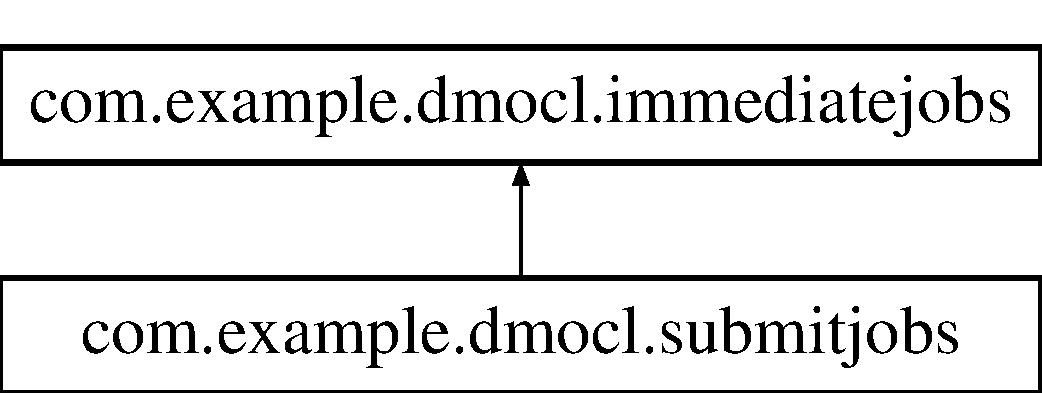
\includegraphics[height=2.000000cm]{classcom_1_1example_1_1dmocl_1_1submitjobs}
\end{center}
\end{figure}
\subsection*{Public Member Functions}
\begin{DoxyCompactItemize}
\item 
\mbox{\Hypertarget{classcom_1_1example_1_1dmocl_1_1submitjobs_a482225e911b94fb9ffd69233fc457800}\label{classcom_1_1example_1_1dmocl_1_1submitjobs_a482225e911b94fb9ffd69233fc457800}} 
{\bfseries submitjobs} (Handler result\+Handler, Executor executor, Context context, Text\+View jobinfo, Button startbutton, String G\+P\+Upath, boolean doexport, boolean dolog, boolean appendresults, String logfn, String fn, String mode, int clusterno, int passes, int clusi, int features, String kmeanseps, String dbscaneps, int dbscanneigh, boolean G\+P\+Ufound, int cores)
\item 
\mbox{\Hypertarget{classcom_1_1example_1_1dmocl_1_1submitjobs_a79402efd281c3fe0a661998d5874791c}\label{classcom_1_1example_1_1dmocl_1_1submitjobs_a79402efd281c3fe0a661998d5874791c}} 
void {\bfseries startcalculations} ()
\item 
\mbox{\Hypertarget{classcom_1_1example_1_1dmocl_1_1submitjobs_ac1d6ef36ed662cda753e0d884b596a04}\label{classcom_1_1example_1_1dmocl_1_1submitjobs_ac1d6ef36ed662cda753e0d884b596a04}} 
void {\bfseries startsubmitjobs} (final Repository\+Callback$<$ jobschedresponse $>$ callback)
\end{DoxyCompactItemize}
\subsection*{Additional Inherited Members}


The documentation for this class was generated from the following file\+:\begin{DoxyCompactItemize}
\item 
/home/robert/\+Android\+Studio\+Projects/\+D\+M\+G\+P\+U/app/src/main/java/com/example/dmocl/submitjobs.\+java\end{DoxyCompactItemize}

\chapter{File Documentation}
\hypertarget{AndroidOpenCL_8h}{}\section{/home/robert/\+Android\+Studio\+Projects/\+D\+M\+G\+P\+U/app/src/\+C/include/\+Android\+Open\+CL.h File Reference}
\label{AndroidOpenCL_8h}\index{/home/robert/\+Android\+Studio\+Projects/\+D\+M\+G\+P\+U/app/src/\+C/include/\+Android\+Open\+C\+L.\+h@{/home/robert/\+Android\+Studio\+Projects/\+D\+M\+G\+P\+U/app/src/\+C/include/\+Android\+Open\+C\+L.\+h}}


Load/\+Unload method prototypes.  


\subsection*{Functions}
\begin{DoxyCompactItemize}
\item 
int \mbox{\hyperlink{AndroidOpenCL_8h_ab6b28f57b7a3dbe0c36d66e0a664579d}{load\+Open\+CL}} (const char $\ast$c)
\begin{DoxyCompactList}\small\item\em Loads the Open\+CL library of the Android device dynamically. \end{DoxyCompactList}\item 
void \mbox{\hyperlink{AndroidOpenCL_8h_aca6b9e2ffc2c41c354d0d1663a6725c8}{unload\+Open\+CL}} (void)
\begin{DoxyCompactList}\small\item\em Unloads the Open\+CL library. \end{DoxyCompactList}\end{DoxyCompactItemize}


\subsection{Detailed Description}
Load/\+Unload method prototypes. 

This headerfile contains two method definitions for loading and unloading the Open\+CL shared library.. \begin{DoxyCopyright}{Copyright}
Copyright Robert Fritze 2021 
\end{DoxyCopyright}
\begin{DoxyParagraph}{License\+:}
M\+IT 
\end{DoxyParagraph}
\begin{DoxyVersion}{Version}
1.\+0 
\end{DoxyVersion}
\begin{DoxyAuthor}{Author}
Robert Fritze 
\end{DoxyAuthor}
\begin{DoxyDate}{Date}
11.\+9.\+2021 
\end{DoxyDate}


\subsection{Function Documentation}
\mbox{\Hypertarget{AndroidOpenCL_8h_ab6b28f57b7a3dbe0c36d66e0a664579d}\label{AndroidOpenCL_8h_ab6b28f57b7a3dbe0c36d66e0a664579d}} 
\index{Android\+Open\+C\+L.\+h@{Android\+Open\+C\+L.\+h}!load\+Open\+CL@{load\+Open\+CL}}
\index{load\+Open\+CL@{load\+Open\+CL}!Android\+Open\+C\+L.\+h@{Android\+Open\+C\+L.\+h}}
\subsubsection{\texorpdfstring{load\+Open\+C\+L()}{loadOpenCL()}}
{\footnotesize\ttfamily int load\+Open\+CL (\begin{DoxyParamCaption}\item[{const char $\ast$}]{c }\end{DoxyParamCaption})}



Loads the Open\+CL library of the Android device dynamically. 

Loads the Open\+CL library dynamically. This function {\bfseries M\+U\+ST} be called exactly once before any other call to an Open\+CL function. The function stores the path of the library. If the library has already been loaded, a call to this method will have no effect. Any call to an Open\+CL function without prior call to this method will result in an error. 
\begin{DoxyParams}{Parameters}
{\em c} & (in) Pointer to the path and name of the Open\+C\+L-\/library on the device (can be reused after the call) \\
\hline
\end{DoxyParams}
\begin{DoxyReturn}{Returns}
OK\+: 0, library has already been loaded\+: -\/1, unable to load library\+: -\/2 
\end{DoxyReturn}
\begin{DoxyParagraph}{Multithreading\+:}
fully threadsafe 
\end{DoxyParagraph}
\mbox{\Hypertarget{AndroidOpenCL_8h_aca6b9e2ffc2c41c354d0d1663a6725c8}\label{AndroidOpenCL_8h_aca6b9e2ffc2c41c354d0d1663a6725c8}} 
\index{Android\+Open\+C\+L.\+h@{Android\+Open\+C\+L.\+h}!unload\+Open\+CL@{unload\+Open\+CL}}
\index{unload\+Open\+CL@{unload\+Open\+CL}!Android\+Open\+C\+L.\+h@{Android\+Open\+C\+L.\+h}}
\subsubsection{\texorpdfstring{unload\+Open\+C\+L()}{unloadOpenCL()}}
{\footnotesize\ttfamily void unload\+Open\+CL (\begin{DoxyParamCaption}\item[{void}]{ }\end{DoxyParamCaption})}



Unloads the Open\+CL library. 

This function unloads the library. \begin{DoxyParagraph}{Multithreading\+:}
fully threadsafe 
\end{DoxyParagraph}

\hypertarget{dbscan__c_8h}{}\section{/home/robert/\+Android\+Studio\+Projects/\+D\+M\+G\+P\+U/app/src/\+C/include/dbscan\+\_\+c.h File Reference}
\label{dbscan__c_8h}\index{/home/robert/\+Android\+Studio\+Projects/\+D\+M\+G\+P\+U/app/src/\+C/include/dbscan\+\_\+c.\+h@{/home/robert/\+Android\+Studio\+Projects/\+D\+M\+G\+P\+U/app/src/\+C/include/dbscan\+\_\+c.\+h}}


Header file for the C/\+C+\+G\+PU implementations of the D\+B\+S\+C\+AN algorithm.  


{\ttfamily \#include $<$jni.\+h$>$}\newline
\subsection*{Functions}
\begin{DoxyCompactItemize}
\item 
J\+N\+I\+E\+X\+P\+O\+RT jshort J\+N\+I\+C\+A\+LL \mbox{\hyperlink{dbscan__c_8h_ac96946a3590e41c2ba686a783d2c59c5}{Java\+\_\+com\+\_\+example\+\_\+dmocl\+\_\+dbscan\+\_\+dbscan\+\_\+1c}} (J\+N\+I\+Env $\ast$env, jclass jc, jshort\+Array b, jfloat\+Array rf, jfloat eps, jint kk, jint features)
\item 
J\+N\+I\+E\+X\+P\+O\+RT jshort J\+N\+I\+C\+A\+LL \mbox{\hyperlink{dbscan__c_8h_a279dd21557bcbe8fcb980459a9e46131}{Java\+\_\+com\+\_\+example\+\_\+dmocl\+\_\+dbscan\+\_\+dbscan\+\_\+1c\+\_\+1gpu}} (J\+N\+I\+Env $\ast$env, jclass jc, jshort\+Array b, jfloat\+Array rf, jfloat eps, jint kk, jint features, jlong\+Array e)
\item 
J\+N\+I\+E\+X\+P\+O\+RT jshort J\+N\+I\+C\+A\+LL \mbox{\hyperlink{dbscan__c_8h_a5e0b673d019dfe5d8dbc901adab3f34a}{Java\+\_\+com\+\_\+example\+\_\+dmocl\+\_\+dbscan\+\_\+dbscan\+\_\+1c\+\_\+1phtreads}} (J\+N\+I\+Env $\ast$env, jclass jc, jshort\+Array b, jfloat\+Array rf, jfloat eps, jint kk, jint features, jint cores, jlong\+Array e)
\end{DoxyCompactItemize}


\subsection{Detailed Description}
Header file for the C/\+C+\+G\+PU implementations of the D\+B\+S\+C\+AN algorithm. 

This header file contains three method prototypes, that allow to perform single-\/ or multithreaded C\+PU or G\+PU based D\+B\+S\+C\+AN cluster searches. \begin{DoxyCopyright}{Copyright}
Copyright Robert Fritze 2021 
\end{DoxyCopyright}
\begin{DoxyParagraph}{License\+:}
M\+IT 
\end{DoxyParagraph}
\begin{DoxyVersion}{Version}
1.\+0 
\end{DoxyVersion}
\begin{DoxyAuthor}{Author}
Robert Fritze 
\end{DoxyAuthor}
\begin{DoxyWarning}{Warning}
This file is machine generated 
\end{DoxyWarning}
\begin{DoxyDate}{Date}
11.\+9.\+2021 
\end{DoxyDate}


\subsection{Function Documentation}
\mbox{\Hypertarget{dbscan__c_8h_ac96946a3590e41c2ba686a783d2c59c5}\label{dbscan__c_8h_ac96946a3590e41c2ba686a783d2c59c5}} 
\index{dbscan\+\_\+c.\+h@{dbscan\+\_\+c.\+h}!Java\+\_\+com\+\_\+example\+\_\+dmocl\+\_\+dbscan\+\_\+dbscan\+\_\+1c@{Java\+\_\+com\+\_\+example\+\_\+dmocl\+\_\+dbscan\+\_\+dbscan\+\_\+1c}}
\index{Java\+\_\+com\+\_\+example\+\_\+dmocl\+\_\+dbscan\+\_\+dbscan\+\_\+1c@{Java\+\_\+com\+\_\+example\+\_\+dmocl\+\_\+dbscan\+\_\+dbscan\+\_\+1c}!dbscan\+\_\+c.\+h@{dbscan\+\_\+c.\+h}}
\subsubsection{\texorpdfstring{Java\+\_\+com\+\_\+example\+\_\+dmocl\+\_\+dbscan\+\_\+dbscan\+\_\+1c()}{Java\_com\_example\_dmocl\_dbscan\_dbscan\_1c()}}
{\footnotesize\ttfamily J\+N\+I\+E\+X\+P\+O\+RT jshort J\+N\+I\+C\+A\+LL Java\+\_\+com\+\_\+example\+\_\+dmocl\+\_\+dbscan\+\_\+dbscan\+\_\+1c (\begin{DoxyParamCaption}\item[{J\+N\+I\+Env $\ast$}]{env,  }\item[{jclass}]{jc,  }\item[{jshort\+Array}]{b,  }\item[{jfloat\+Array}]{rf,  }\item[{jfloat}]{eps,  }\item[{jint}]{kk,  }\item[{jint}]{features }\end{DoxyParamCaption})}

Performs a D\+B\+S\+C\+AN cluster search on the input data with one thread. 
\begin{DoxyParams}{Parameters}
{\em env} & J\+NI environment variable \\
\hline
{\em jc} & J\+NI class variable \\
\hline
{\em b} & (out) Array of cluster numbers (0=noise point) \\
\hline
{\em rf} & (in) Array of data points \\
\hline
{\em eps} & search radius \\
\hline
{\em kk} & number of neighbours \\
\hline
{\em features} & number of features per data item contained in the data array \\
\hline
\end{DoxyParams}
\begin{DoxyReturn}{Returns}
number of clusters found (can be zero if only noise points have been detected) or -\/ if negative -\/ an error code 
\end{DoxyReturn}
\begin{DoxyParagraph}{Multithreading\+:}
fully threadsafe 
\end{DoxyParagraph}
\mbox{\Hypertarget{dbscan__c_8h_a279dd21557bcbe8fcb980459a9e46131}\label{dbscan__c_8h_a279dd21557bcbe8fcb980459a9e46131}} 
\index{dbscan\+\_\+c.\+h@{dbscan\+\_\+c.\+h}!Java\+\_\+com\+\_\+example\+\_\+dmocl\+\_\+dbscan\+\_\+dbscan\+\_\+1c\+\_\+1gpu@{Java\+\_\+com\+\_\+example\+\_\+dmocl\+\_\+dbscan\+\_\+dbscan\+\_\+1c\+\_\+1gpu}}
\index{Java\+\_\+com\+\_\+example\+\_\+dmocl\+\_\+dbscan\+\_\+dbscan\+\_\+1c\+\_\+1gpu@{Java\+\_\+com\+\_\+example\+\_\+dmocl\+\_\+dbscan\+\_\+dbscan\+\_\+1c\+\_\+1gpu}!dbscan\+\_\+c.\+h@{dbscan\+\_\+c.\+h}}
\subsubsection{\texorpdfstring{Java\+\_\+com\+\_\+example\+\_\+dmocl\+\_\+dbscan\+\_\+dbscan\+\_\+1c\+\_\+1gpu()}{Java\_com\_example\_dmocl\_dbscan\_dbscan\_1c\_1gpu()}}
{\footnotesize\ttfamily J\+N\+I\+E\+X\+P\+O\+RT jshort J\+N\+I\+C\+A\+LL Java\+\_\+com\+\_\+example\+\_\+dmocl\+\_\+dbscan\+\_\+dbscan\+\_\+1c\+\_\+1gpu (\begin{DoxyParamCaption}\item[{J\+N\+I\+Env $\ast$}]{env,  }\item[{jclass}]{jc,  }\item[{jshort\+Array}]{b,  }\item[{jfloat\+Array}]{rf,  }\item[{jfloat}]{eps,  }\item[{jint}]{kk,  }\item[{jint}]{features,  }\item[{jlong\+Array}]{e }\end{DoxyParamCaption})}

Performs a D\+B\+S\+C\+AN cluster search on the G\+PU. 
\begin{DoxyParams}{Parameters}
{\em env} & J\+NI environment variable \\
\hline
{\em jc} & J\+NI class variable \\
\hline
{\em b} & (out) Array of cluster numbers (0=noise point) \\
\hline
{\em rf} & (in) Array of data points \\
\hline
{\em eps} & search radius \\
\hline
{\em kk} & number of neighbours \\
\hline
{\em features} & number of features per data item contained in the data array \\
\hline
{\em e} & (out) Array of exactly one long value, contains the exclusive time needed (in ns) \\
\hline
\end{DoxyParams}
\begin{DoxyReturn}{Returns}
number of clusters found (can be zero if only noise points have been detected) or -\/ if negative -\/ an error code 
\end{DoxyReturn}
\begin{DoxyParagraph}{Multithreading\+:}
fully threadsafe 
\end{DoxyParagraph}
\mbox{\Hypertarget{dbscan__c_8h_a5e0b673d019dfe5d8dbc901adab3f34a}\label{dbscan__c_8h_a5e0b673d019dfe5d8dbc901adab3f34a}} 
\index{dbscan\+\_\+c.\+h@{dbscan\+\_\+c.\+h}!Java\+\_\+com\+\_\+example\+\_\+dmocl\+\_\+dbscan\+\_\+dbscan\+\_\+1c\+\_\+1phtreads@{Java\+\_\+com\+\_\+example\+\_\+dmocl\+\_\+dbscan\+\_\+dbscan\+\_\+1c\+\_\+1phtreads}}
\index{Java\+\_\+com\+\_\+example\+\_\+dmocl\+\_\+dbscan\+\_\+dbscan\+\_\+1c\+\_\+1phtreads@{Java\+\_\+com\+\_\+example\+\_\+dmocl\+\_\+dbscan\+\_\+dbscan\+\_\+1c\+\_\+1phtreads}!dbscan\+\_\+c.\+h@{dbscan\+\_\+c.\+h}}
\subsubsection{\texorpdfstring{Java\+\_\+com\+\_\+example\+\_\+dmocl\+\_\+dbscan\+\_\+dbscan\+\_\+1c\+\_\+1phtreads()}{Java\_com\_example\_dmocl\_dbscan\_dbscan\_1c\_1phtreads()}}
{\footnotesize\ttfamily J\+N\+I\+E\+X\+P\+O\+RT jshort J\+N\+I\+C\+A\+LL Java\+\_\+com\+\_\+example\+\_\+dmocl\+\_\+dbscan\+\_\+dbscan\+\_\+1c\+\_\+1phtreads (\begin{DoxyParamCaption}\item[{J\+N\+I\+Env $\ast$}]{env,  }\item[{jclass}]{jc,  }\item[{jshort\+Array}]{b,  }\item[{jfloat\+Array}]{rf,  }\item[{jfloat}]{eps,  }\item[{jint}]{kk,  }\item[{jint}]{features,  }\item[{jint}]{cores,  }\item[{jlong\+Array}]{e }\end{DoxyParamCaption})}

Performs a D\+B\+S\+C\+AN cluster search on the input data with multiple threads. 
\begin{DoxyParams}{Parameters}
{\em env} & J\+NI environment variable \\
\hline
{\em jc} & J\+NI class variable \\
\hline
{\em b} & (out) Array of cluster numbers (0=noise point) \\
\hline
{\em rf} & (in) Array of data points \\
\hline
{\em eps} & search radius \\
\hline
{\em kk} & number of neighbours \\
\hline
{\em features} & number of features per data item contained in the data array \\
\hline
{\em cores} & number of cores that should be used \\
\hline
{\em e} & (out) Array of exactly one long value, contains the exclusive time needed (in ns) \\
\hline
\end{DoxyParams}
\begin{DoxyReturn}{Returns}
number of clusters found (can be zero if only noise points have been detected) or -\/ if negative -\/ an error code 
\end{DoxyReturn}
\begin{DoxyParagraph}{Multithreading\+:}
fully threadsafe 
\end{DoxyParagraph}

\hypertarget{kmeans__c_8h}{}\section{/home/robert/\+Android\+Studio\+Projects/\+D\+M\+G\+P\+U/app/src/\+C/include/kmeans\+\_\+c.h File Reference}
\label{kmeans__c_8h}\index{/home/robert/\+Android\+Studio\+Projects/\+D\+M\+G\+P\+U/app/src/\+C/include/kmeans\+\_\+c.\+h@{/home/robert/\+Android\+Studio\+Projects/\+D\+M\+G\+P\+U/app/src/\+C/include/kmeans\+\_\+c.\+h}}


Header file for the C/\+C+\+G\+PU implementations of the Kmeans algorithm.  


{\ttfamily \#include $<$jni.\+h$>$}\newline
\subsection*{Functions}
\begin{DoxyCompactItemize}
\item 
J\+N\+I\+E\+X\+P\+O\+RT jshort J\+N\+I\+C\+A\+LL \mbox{\hyperlink{kmeans__c_8h_a8d358801f2beeb2c15237e2a1a98500f}{Java\+\_\+com\+\_\+example\+\_\+dmocl\+\_\+kmeans\+\_\+kmeans\+\_\+1c}} (J\+N\+I\+Env $\ast$env, jclass jc, jshort\+Array b, jfloat\+Array rf, jfloat eps, jint kk, jint features)
\item 
J\+N\+I\+E\+X\+P\+O\+RT jshort J\+N\+I\+C\+A\+LL \mbox{\hyperlink{kmeans__c_8h_adcd1210c788d0762e4f4362dc32dba4e}{Java\+\_\+com\+\_\+example\+\_\+dmocl\+\_\+kmeans\+\_\+kmeans\+\_\+1c\+\_\+1gpu}} (J\+N\+I\+Env $\ast$env, jclass jc, jshort\+Array b, jfloat\+Array rf, jfloat eps, jint cluno, jint features, jlong\+Array e)
\item 
J\+N\+I\+E\+X\+P\+O\+RT jshort J\+N\+I\+C\+A\+LL \mbox{\hyperlink{kmeans__c_8h_a226636af0647863759dce78b63c717f1}{Java\+\_\+com\+\_\+example\+\_\+dmocl\+\_\+kmeans\+\_\+kmeans\+\_\+1c\+\_\+1phtreads}} (J\+N\+I\+Env $\ast$env, jclass jc, jshort\+Array b, jfloat\+Array rf, jfloat eps, jint cluno, jint features, jint cores, jlong\+Array e)
\item 
J\+N\+I\+E\+X\+P\+O\+RT void J\+N\+I\+C\+A\+LL \mbox{\hyperlink{kmeans__c_8h_a158e27ece530f3be8289b75fdd47257f}{Java\+\_\+com\+\_\+example\+\_\+dmocl\+\_\+kmeans\+\_\+kmabort\+\_\+1c}} (J\+N\+I\+Env $\ast$env, jclass clazz)
\item 
J\+N\+I\+E\+X\+P\+O\+RT void J\+N\+I\+C\+A\+LL \mbox{\hyperlink{kmeans__c_8h_a2e491512385eeb5b60e98a0922ccb23a}{Java\+\_\+com\+\_\+example\+\_\+dmocl\+\_\+kmeans\+\_\+kmresume\+\_\+1c}} (J\+N\+I\+Env $\ast$env, jclass clazz)
\end{DoxyCompactItemize}


\subsection{Detailed Description}
Header file for the C/\+C+\+G\+PU implementations of the Kmeans algorithm. 

This header file contains three method prototypes, that allow to perform single-\/ or multithreaded C\+PU or G\+PU based Kmeans cluster searches. \begin{DoxyCopyright}{Copyright}
Copyright Robert Fritze 2021 
\end{DoxyCopyright}
\begin{DoxyParagraph}{License\+:}
M\+IT 
\end{DoxyParagraph}
\begin{DoxyVersion}{Version}
1.\+0 
\end{DoxyVersion}
\begin{DoxyAuthor}{Author}
Robert Fritze 
\end{DoxyAuthor}
\begin{DoxyWarning}{Warning}
This file is machine generated 
\end{DoxyWarning}
\begin{DoxyDate}{Date}
11.\+9.\+2021 
\end{DoxyDate}


\subsection{Function Documentation}
\mbox{\Hypertarget{kmeans__c_8h_a158e27ece530f3be8289b75fdd47257f}\label{kmeans__c_8h_a158e27ece530f3be8289b75fdd47257f}} 
\index{kmeans\+\_\+c.\+h@{kmeans\+\_\+c.\+h}!Java\+\_\+com\+\_\+example\+\_\+dmocl\+\_\+kmeans\+\_\+kmabort\+\_\+1c@{Java\+\_\+com\+\_\+example\+\_\+dmocl\+\_\+kmeans\+\_\+kmabort\+\_\+1c}}
\index{Java\+\_\+com\+\_\+example\+\_\+dmocl\+\_\+kmeans\+\_\+kmabort\+\_\+1c@{Java\+\_\+com\+\_\+example\+\_\+dmocl\+\_\+kmeans\+\_\+kmabort\+\_\+1c}!kmeans\+\_\+c.\+h@{kmeans\+\_\+c.\+h}}
\subsubsection{\texorpdfstring{Java\+\_\+com\+\_\+example\+\_\+dmocl\+\_\+kmeans\+\_\+kmabort\+\_\+1c()}{Java\_com\_example\_dmocl\_kmeans\_kmabort\_1c()}}
{\footnotesize\ttfamily J\+N\+I\+E\+X\+P\+O\+RT void J\+N\+I\+C\+A\+LL Java\+\_\+com\+\_\+example\+\_\+dmocl\+\_\+kmeans\+\_\+kmabort\+\_\+1c (\begin{DoxyParamCaption}\item[{J\+N\+I\+Env $\ast$}]{env,  }\item[{jclass}]{clazz }\end{DoxyParamCaption})}

Signals all running Kmeans algorithms to abort immediately. Any new Kmeans cluster search will be aborted imediately. \begin{DoxyWarning}{Warning}
This function acts on a \textquotesingle{}global\textquotesingle{} scale\+: All callers that use this library will not be any more able to make calls to the library functions of this library. 
\end{DoxyWarning}

\begin{DoxyParams}{Parameters}
{\em env} & J\+NI environment variable \\
\hline
{\em clazz} & J\+NI class variable \\
\hline
\end{DoxyParams}
\begin{DoxyParagraph}{Multithreading\+:}
fully threadsafe 
\end{DoxyParagraph}
\mbox{\Hypertarget{kmeans__c_8h_a8d358801f2beeb2c15237e2a1a98500f}\label{kmeans__c_8h_a8d358801f2beeb2c15237e2a1a98500f}} 
\index{kmeans\+\_\+c.\+h@{kmeans\+\_\+c.\+h}!Java\+\_\+com\+\_\+example\+\_\+dmocl\+\_\+kmeans\+\_\+kmeans\+\_\+1c@{Java\+\_\+com\+\_\+example\+\_\+dmocl\+\_\+kmeans\+\_\+kmeans\+\_\+1c}}
\index{Java\+\_\+com\+\_\+example\+\_\+dmocl\+\_\+kmeans\+\_\+kmeans\+\_\+1c@{Java\+\_\+com\+\_\+example\+\_\+dmocl\+\_\+kmeans\+\_\+kmeans\+\_\+1c}!kmeans\+\_\+c.\+h@{kmeans\+\_\+c.\+h}}
\subsubsection{\texorpdfstring{Java\+\_\+com\+\_\+example\+\_\+dmocl\+\_\+kmeans\+\_\+kmeans\+\_\+1c()}{Java\_com\_example\_dmocl\_kmeans\_kmeans\_1c()}}
{\footnotesize\ttfamily J\+N\+I\+E\+X\+P\+O\+RT jshort J\+N\+I\+C\+A\+LL Java\+\_\+com\+\_\+example\+\_\+dmocl\+\_\+kmeans\+\_\+kmeans\+\_\+1c (\begin{DoxyParamCaption}\item[{J\+N\+I\+Env $\ast$}]{env,  }\item[{jclass}]{jc,  }\item[{jshort\+Array}]{b,  }\item[{jfloat\+Array}]{rf,  }\item[{jfloat}]{eps,  }\item[{jint}]{kk,  }\item[{jint}]{features }\end{DoxyParamCaption})}

Performs a Kmeans cluster search on the C\+PU (one thread). 
\begin{DoxyParams}{Parameters}
{\em env} & J\+NI environment variable \\
\hline
{\em jc} & J\+NI class variable \\
\hline
{\em b} & (out) Array of cluster numbers (0=noise point) \\
\hline
{\em rf} & (in) Array of data points \\
\hline
{\em eps} & search radius \\
\hline
{\em kk} & number of clusters to search for \\
\hline
{\em features} & number of features per data item contained in the data array \\
\hline
\end{DoxyParams}
\begin{DoxyReturn}{Returns}
0 = no error, $<$0 = error number 
\end{DoxyReturn}
\begin{DoxyParagraph}{Multithreading\+:}
fully threadsafe 
\end{DoxyParagraph}
\mbox{\Hypertarget{kmeans__c_8h_adcd1210c788d0762e4f4362dc32dba4e}\label{kmeans__c_8h_adcd1210c788d0762e4f4362dc32dba4e}} 
\index{kmeans\+\_\+c.\+h@{kmeans\+\_\+c.\+h}!Java\+\_\+com\+\_\+example\+\_\+dmocl\+\_\+kmeans\+\_\+kmeans\+\_\+1c\+\_\+1gpu@{Java\+\_\+com\+\_\+example\+\_\+dmocl\+\_\+kmeans\+\_\+kmeans\+\_\+1c\+\_\+1gpu}}
\index{Java\+\_\+com\+\_\+example\+\_\+dmocl\+\_\+kmeans\+\_\+kmeans\+\_\+1c\+\_\+1gpu@{Java\+\_\+com\+\_\+example\+\_\+dmocl\+\_\+kmeans\+\_\+kmeans\+\_\+1c\+\_\+1gpu}!kmeans\+\_\+c.\+h@{kmeans\+\_\+c.\+h}}
\subsubsection{\texorpdfstring{Java\+\_\+com\+\_\+example\+\_\+dmocl\+\_\+kmeans\+\_\+kmeans\+\_\+1c\+\_\+1gpu()}{Java\_com\_example\_dmocl\_kmeans\_kmeans\_1c\_1gpu()}}
{\footnotesize\ttfamily J\+N\+I\+E\+X\+P\+O\+RT jshort J\+N\+I\+C\+A\+LL Java\+\_\+com\+\_\+example\+\_\+dmocl\+\_\+kmeans\+\_\+kmeans\+\_\+1c\+\_\+1gpu (\begin{DoxyParamCaption}\item[{J\+N\+I\+Env $\ast$}]{env,  }\item[{jclass}]{jc,  }\item[{jshort\+Array}]{b,  }\item[{jfloat\+Array}]{rf,  }\item[{jfloat}]{eps,  }\item[{jint}]{cluno,  }\item[{jint}]{features,  }\item[{jlong\+Array}]{e }\end{DoxyParamCaption})}

Performs a Kmeans cluster search on the G\+PU. 
\begin{DoxyParams}{Parameters}
{\em env} & J\+NI environment variable \\
\hline
{\em jc} & J\+NI class variable \\
\hline
{\em b} & (out) Array of cluster numbers (0=noise point) \\
\hline
{\em rf} & (in) Array of data points \\
\hline
{\em eps} & search radius \\
\hline
{\em cluno} & number of clusters to search for \\
\hline
{\em features} & number of features per data item contained in the data array \\
\hline
{\em e} & (out) Array of exactly one long value, contains the exclusive time needed (in ns) \\
\hline
\end{DoxyParams}
\begin{DoxyReturn}{Returns}
0 = no error, $<$0 = error number 
\end{DoxyReturn}
\begin{DoxyParagraph}{Multithreading\+:}
fully threadsafe 
\end{DoxyParagraph}
\mbox{\Hypertarget{kmeans__c_8h_a226636af0647863759dce78b63c717f1}\label{kmeans__c_8h_a226636af0647863759dce78b63c717f1}} 
\index{kmeans\+\_\+c.\+h@{kmeans\+\_\+c.\+h}!Java\+\_\+com\+\_\+example\+\_\+dmocl\+\_\+kmeans\+\_\+kmeans\+\_\+1c\+\_\+1phtreads@{Java\+\_\+com\+\_\+example\+\_\+dmocl\+\_\+kmeans\+\_\+kmeans\+\_\+1c\+\_\+1phtreads}}
\index{Java\+\_\+com\+\_\+example\+\_\+dmocl\+\_\+kmeans\+\_\+kmeans\+\_\+1c\+\_\+1phtreads@{Java\+\_\+com\+\_\+example\+\_\+dmocl\+\_\+kmeans\+\_\+kmeans\+\_\+1c\+\_\+1phtreads}!kmeans\+\_\+c.\+h@{kmeans\+\_\+c.\+h}}
\subsubsection{\texorpdfstring{Java\+\_\+com\+\_\+example\+\_\+dmocl\+\_\+kmeans\+\_\+kmeans\+\_\+1c\+\_\+1phtreads()}{Java\_com\_example\_dmocl\_kmeans\_kmeans\_1c\_1phtreads()}}
{\footnotesize\ttfamily J\+N\+I\+E\+X\+P\+O\+RT jshort J\+N\+I\+C\+A\+LL Java\+\_\+com\+\_\+example\+\_\+dmocl\+\_\+kmeans\+\_\+kmeans\+\_\+1c\+\_\+1phtreads (\begin{DoxyParamCaption}\item[{J\+N\+I\+Env $\ast$}]{env,  }\item[{jclass}]{jc,  }\item[{jshort\+Array}]{b,  }\item[{jfloat\+Array}]{rf,  }\item[{jfloat}]{eps,  }\item[{jint}]{cluno,  }\item[{jint}]{features,  }\item[{jint}]{cores,  }\item[{jlong\+Array}]{e }\end{DoxyParamCaption})}

Performs a Kmeans cluster search on the C\+PU (multiple threads). 
\begin{DoxyParams}{Parameters}
{\em env} & J\+NI environment variable \\
\hline
{\em jc} & J\+NI class variable \\
\hline
{\em b} & (out) Array of cluster numbers \\
\hline
{\em rf} & (in) Array of data points \\
\hline
{\em eps} & search radius \\
\hline
{\em cluno} & numbers of clusters that should be found \\
\hline
{\em features} & number of features per data item contained in the data array \\
\hline
{\em cores} & number of cores that should be used \\
\hline
{\em e} & (out) Array of exactly one long value, contains the exclusive time needed (in ns) \\
\hline
\end{DoxyParams}
\begin{DoxyReturn}{Returns}
0 = no error, $<$0 = error number 
\end{DoxyReturn}
\begin{DoxyParagraph}{Multithreading\+:}
fully threadsafe 
\end{DoxyParagraph}
\mbox{\Hypertarget{kmeans__c_8h_a2e491512385eeb5b60e98a0922ccb23a}\label{kmeans__c_8h_a2e491512385eeb5b60e98a0922ccb23a}} 
\index{kmeans\+\_\+c.\+h@{kmeans\+\_\+c.\+h}!Java\+\_\+com\+\_\+example\+\_\+dmocl\+\_\+kmeans\+\_\+kmresume\+\_\+1c@{Java\+\_\+com\+\_\+example\+\_\+dmocl\+\_\+kmeans\+\_\+kmresume\+\_\+1c}}
\index{Java\+\_\+com\+\_\+example\+\_\+dmocl\+\_\+kmeans\+\_\+kmresume\+\_\+1c@{Java\+\_\+com\+\_\+example\+\_\+dmocl\+\_\+kmeans\+\_\+kmresume\+\_\+1c}!kmeans\+\_\+c.\+h@{kmeans\+\_\+c.\+h}}
\subsubsection{\texorpdfstring{Java\+\_\+com\+\_\+example\+\_\+dmocl\+\_\+kmeans\+\_\+kmresume\+\_\+1c()}{Java\_com\_example\_dmocl\_kmeans\_kmresume\_1c()}}
{\footnotesize\ttfamily J\+N\+I\+E\+X\+P\+O\+RT void J\+N\+I\+C\+A\+LL Java\+\_\+com\+\_\+example\+\_\+dmocl\+\_\+kmeans\+\_\+kmresume\+\_\+1c (\begin{DoxyParamCaption}\item[{J\+N\+I\+Env $\ast$}]{env,  }\item[{jclass}]{clazz }\end{DoxyParamCaption})}

Allows to make new Kmeans cluster searches. \begin{DoxyWarning}{Warning}
This function acts on a \textquotesingle{}global\textquotesingle{} scale. It reverts the effect of Java\+\_\+com\+\_\+example\+\_\+dmocl\+\_\+kmeans\+\_\+kmabort\+\_\+1c. 
\end{DoxyWarning}

\begin{DoxyParams}{Parameters}
{\em env} & J\+NI environment variable \\
\hline
{\em clazz} & J\+NI class variable \\
\hline
\end{DoxyParams}
\begin{DoxyParagraph}{Multithreading\+:}
fully threadsafe 
\end{DoxyParagraph}

\hypertarget{oclwrapper_8h}{}\section{/home/robert/\+Android\+Studio\+Projects/\+D\+M\+G\+P\+U/app/src/\+C/include/oclwrapper.h File Reference}
\label{oclwrapper_8h}\index{/home/robert/\+Android\+Studio\+Projects/\+D\+M\+G\+P\+U/app/src/\+C/include/oclwrapper.\+h@{/home/robert/\+Android\+Studio\+Projects/\+D\+M\+G\+P\+U/app/src/\+C/include/oclwrapper.\+h}}


Defines the default target Open\+CL version.  


\subsection*{Macros}
\begin{DoxyCompactItemize}
\item 
\mbox{\Hypertarget{oclwrapper_8h_ac1ae4add974b9cfc6b5aaf8a578f01ab}\label{oclwrapper_8h_ac1ae4add974b9cfc6b5aaf8a578f01ab}} 
\#define \mbox{\hyperlink{oclwrapper_8h_ac1ae4add974b9cfc6b5aaf8a578f01ab}{U\+N\+K\+N\+O\+WN}}~-\/1
\begin{DoxyCompactList}\small\item\em unknown architecture \end{DoxyCompactList}\item 
\mbox{\Hypertarget{oclwrapper_8h_ab026c2caefe5237d3ff08d64bc44f031}\label{oclwrapper_8h_ab026c2caefe5237d3ff08d64bc44f031}} 
\#define \mbox{\hyperlink{oclwrapper_8h_ab026c2caefe5237d3ff08d64bc44f031}{A\+R\+M32}}~0
\begin{DoxyCompactList}\small\item\em arm-\/v7 \end{DoxyCompactList}\item 
\mbox{\Hypertarget{oclwrapper_8h_ad60f4509a26d03acf44e10243332242d}\label{oclwrapper_8h_ad60f4509a26d03acf44e10243332242d}} 
\#define \mbox{\hyperlink{oclwrapper_8h_ad60f4509a26d03acf44e10243332242d}{A\+R\+M64}}~1
\begin{DoxyCompactList}\small\item\em arm-\/v8 \end{DoxyCompactList}\item 
\mbox{\Hypertarget{oclwrapper_8h_ab45f50b8e38b9c733084c4557b34b760}\label{oclwrapper_8h_ab45f50b8e38b9c733084c4557b34b760}} 
\#define \mbox{\hyperlink{oclwrapper_8h_ab45f50b8e38b9c733084c4557b34b760}{I\+N\+T\+E\+L32}}~2
\begin{DoxyCompactList}\small\item\em intel x86 \end{DoxyCompactList}\item 
\mbox{\Hypertarget{oclwrapper_8h_a274cff70a8ceaa329d01cd651abcf663}\label{oclwrapper_8h_a274cff70a8ceaa329d01cd651abcf663}} 
\#define \mbox{\hyperlink{oclwrapper_8h_a274cff70a8ceaa329d01cd651abcf663}{I\+N\+T\+E\+L64}}~3
\begin{DoxyCompactList}\small\item\em intel x86\+\_\+64 \end{DoxyCompactList}\item 
\mbox{\Hypertarget{oclwrapper_8h_a5990dea19d4ccb046a3d81b311457add}\label{oclwrapper_8h_a5990dea19d4ccb046a3d81b311457add}} 
\#define \mbox{\hyperlink{oclwrapper_8h_a5990dea19d4ccb046a3d81b311457add}{C\+L\+\_\+\+T\+A\+R\+G\+E\+T\+\_\+\+O\+P\+E\+N\+C\+L\+\_\+\+V\+E\+R\+S\+I\+ON}}~120
\begin{DoxyCompactList}\small\item\em the default target Open\+CL version \end{DoxyCompactList}\end{DoxyCompactItemize}
\subsection*{Functions}
\begin{DoxyCompactItemize}
\item 
J\+N\+I\+E\+X\+P\+O\+RT jint J\+N\+I\+C\+A\+LL \mbox{\hyperlink{oclwrapper_8h_a70b9cfe87ec353e0b132686b6ad633c9}{Java\+\_\+com\+\_\+example\+\_\+dmocl\+\_\+oclwrap\+\_\+is\+C\+Lang}} (J\+N\+I\+Env $\ast$env, jclass clazz)
\begin{DoxyCompactList}\small\item\em Checks if C\+L\+A\+NG has been used for compilation. \end{DoxyCompactList}\item 
J\+N\+I\+E\+X\+P\+O\+RT jint J\+N\+I\+C\+A\+LL \mbox{\hyperlink{oclwrapper_8h_a2604db65a63923724d541413d317a384}{Java\+\_\+com\+\_\+example\+\_\+dmocl\+\_\+oclwrap\+\_\+get\+C\+Lmaj}} (J\+N\+I\+Env $\ast$env, jclass clazz)
\begin{DoxyCompactList}\small\item\em Returns the C\+L\+A\+NG major version number. \end{DoxyCompactList}\item 
J\+N\+I\+E\+X\+P\+O\+RT jint J\+N\+I\+C\+A\+LL \mbox{\hyperlink{oclwrapper_8h_adebb34bc4eae343c98f973f900126f65}{Java\+\_\+com\+\_\+example\+\_\+dmocl\+\_\+oclwrap\+\_\+get\+C\+Lmin}} (J\+N\+I\+Env $\ast$env, jclass clazz)
\begin{DoxyCompactList}\small\item\em Returns the C\+L\+A\+NG minor version number. \end{DoxyCompactList}\item 
J\+N\+I\+E\+X\+P\+O\+RT jint J\+N\+I\+C\+A\+LL \mbox{\hyperlink{oclwrapper_8h_ac363dec768880e96246e2f044a3d3d5f}{Java\+\_\+com\+\_\+example\+\_\+dmocl\+\_\+oclwrap\+\_\+get\+C\+Lpatch}} (J\+N\+I\+Env $\ast$env, jclass clazz)
\begin{DoxyCompactList}\small\item\em Returns the C\+L\+A\+NG patch version number. \end{DoxyCompactList}\item 
J\+N\+I\+E\+X\+P\+O\+RT jint J\+N\+I\+C\+A\+LL \mbox{\hyperlink{oclwrapper_8h_ae5fe6385046d0a1b04c33bb7d4592a90}{Java\+\_\+com\+\_\+example\+\_\+dmocl\+\_\+oclwrap\+\_\+load\+Open\+CL}} (J\+N\+I\+Env $\ast$env, jobject thiz, jstring s)
\begin{DoxyCompactList}\small\item\em Java wrapper function to load the native Open\+CL library. \end{DoxyCompactList}\item 
J\+N\+I\+E\+X\+P\+O\+RT void J\+N\+I\+C\+A\+LL \mbox{\hyperlink{oclwrapper_8h_adf50b121c77631f9b73d965a2f20c412}{Java\+\_\+com\+\_\+example\+\_\+dmocl\+\_\+oclwrap\+\_\+unload\+Open\+CL}} (J\+N\+I\+Env $\ast$env, jobject thiz)
\begin{DoxyCompactList}\small\item\em Java wrapper function to unload the native Open\+CL library. \end{DoxyCompactList}\item 
J\+N\+I\+E\+X\+P\+O\+RT jint J\+N\+I\+C\+A\+LL \mbox{\hyperlink{oclwrapper_8h_ac7305f7bd18566b51c337006ada22a52}{Java\+\_\+com\+\_\+example\+\_\+dmocl\+\_\+oclwrap\+\_\+\+Andr\+C\+L\+Get\+Platform\+Cnt}} (J\+N\+I\+Env $\ast$env, jobject thiz)
\begin{DoxyCompactList}\small\item\em Returns the number of Open\+CL platforms. \end{DoxyCompactList}\item 
J\+N\+I\+E\+X\+P\+O\+RT jint J\+N\+I\+C\+A\+LL \mbox{\hyperlink{oclwrapper_8h_a9d2c9ba80285d397a5dfb04785c4a808}{Java\+\_\+com\+\_\+example\+\_\+dmocl\+\_\+oclwrap\+\_\+\+Andr\+C\+L\+Get\+Device\+Cnt}} (J\+N\+I\+Env $\ast$env, jobject thiz, jint i)
\begin{DoxyCompactList}\small\item\em Returns the number of Open\+CL devices for a given platform. \end{DoxyCompactList}\item 
J\+N\+I\+E\+X\+P\+O\+RT jobject J\+N\+I\+C\+A\+LL \mbox{\hyperlink{oclwrapper_8h_a80c31db42eaa9b1d9630e341c47c1009}{Java\+\_\+com\+\_\+example\+\_\+dmocl\+\_\+oclwrap\+\_\+\+Andr\+C\+Lget\+Device\+Name}} (J\+N\+I\+Env $\ast$env, jobject thiz, jint platf, jint dev)
\begin{DoxyCompactList}\small\item\em Returns some info for a given Open\+CL device (and platform number) \end{DoxyCompactList}\item 
J\+N\+I\+E\+X\+P\+O\+RT jint J\+N\+I\+C\+A\+LL \mbox{\hyperlink{oclwrapper_8h_a4f4a70158379b10c5beb9414eec0706f}{Java\+\_\+com\+\_\+example\+\_\+dmocl\+\_\+oclwrap\+\_\+get\+Architecture}} (J\+N\+I\+Env $\ast$env, jclass clazz)
\begin{DoxyCompactList}\small\item\em Returns the C\+PU architecture. \end{DoxyCompactList}\end{DoxyCompactItemize}


\subsection{Detailed Description}
Defines the default target Open\+CL version. 

Defines the default target Open\+CL version \begin{DoxyCopyright}{Copyright}
Copyright Robert Fritze 2021 
\end{DoxyCopyright}
\begin{DoxyParagraph}{License\+:}
M\+IT 
\end{DoxyParagraph}
\begin{DoxyVersion}{Version}
1.\+0 
\end{DoxyVersion}
\begin{DoxyWarning}{Warning}
This header file must be included {\bfseries B\+E\+F\+O\+RE} any Open\+CL header file 
\end{DoxyWarning}
\begin{DoxyAuthor}{Author}
Robert Fritze 
\end{DoxyAuthor}
\begin{DoxyDate}{Date}
11.\+9.\+2021 
\end{DoxyDate}


\subsection{Function Documentation}
\mbox{\Hypertarget{oclwrapper_8h_a9d2c9ba80285d397a5dfb04785c4a808}\label{oclwrapper_8h_a9d2c9ba80285d397a5dfb04785c4a808}} 
\index{oclwrapper.\+h@{oclwrapper.\+h}!Java\+\_\+com\+\_\+example\+\_\+dmocl\+\_\+oclwrap\+\_\+\+Andr\+C\+L\+Get\+Device\+Cnt@{Java\+\_\+com\+\_\+example\+\_\+dmocl\+\_\+oclwrap\+\_\+\+Andr\+C\+L\+Get\+Device\+Cnt}}
\index{Java\+\_\+com\+\_\+example\+\_\+dmocl\+\_\+oclwrap\+\_\+\+Andr\+C\+L\+Get\+Device\+Cnt@{Java\+\_\+com\+\_\+example\+\_\+dmocl\+\_\+oclwrap\+\_\+\+Andr\+C\+L\+Get\+Device\+Cnt}!oclwrapper.\+h@{oclwrapper.\+h}}
\subsubsection{\texorpdfstring{Java\+\_\+com\+\_\+example\+\_\+dmocl\+\_\+oclwrap\+\_\+\+Andr\+C\+L\+Get\+Device\+Cnt()}{Java\_com\_example\_dmocl\_oclwrap\_AndrCLGetDeviceCnt()}}
{\footnotesize\ttfamily J\+N\+I\+E\+X\+P\+O\+RT jint J\+N\+I\+C\+A\+LL Java\+\_\+com\+\_\+example\+\_\+dmocl\+\_\+oclwrap\+\_\+\+Andr\+C\+L\+Get\+Device\+Cnt (\begin{DoxyParamCaption}\item[{J\+N\+I\+Env $\ast$}]{env,  }\item[{jobject}]{thiz,  }\item[{jint}]{i }\end{DoxyParamCaption})}



Returns the number of Open\+CL devices for a given platform. 


\begin{DoxyParams}{Parameters}
{\em env} & pointer to J\+NI environment \\
\hline
{\em thiz} & reference to J\+NI class \\
\hline
{\em i} & platform number \\
\hline
\end{DoxyParams}
\begin{DoxyReturn}{Returns}
$>$=0 number of devices, $<$0 error occurred 
\end{DoxyReturn}
\begin{DoxyParagraph}{Multithreading\+:}
fully threadsafe (if native Open\+CL function is threadsafe) 
\end{DoxyParagraph}
\mbox{\Hypertarget{oclwrapper_8h_a80c31db42eaa9b1d9630e341c47c1009}\label{oclwrapper_8h_a80c31db42eaa9b1d9630e341c47c1009}} 
\index{oclwrapper.\+h@{oclwrapper.\+h}!Java\+\_\+com\+\_\+example\+\_\+dmocl\+\_\+oclwrap\+\_\+\+Andr\+C\+Lget\+Device\+Name@{Java\+\_\+com\+\_\+example\+\_\+dmocl\+\_\+oclwrap\+\_\+\+Andr\+C\+Lget\+Device\+Name}}
\index{Java\+\_\+com\+\_\+example\+\_\+dmocl\+\_\+oclwrap\+\_\+\+Andr\+C\+Lget\+Device\+Name@{Java\+\_\+com\+\_\+example\+\_\+dmocl\+\_\+oclwrap\+\_\+\+Andr\+C\+Lget\+Device\+Name}!oclwrapper.\+h@{oclwrapper.\+h}}
\subsubsection{\texorpdfstring{Java\+\_\+com\+\_\+example\+\_\+dmocl\+\_\+oclwrap\+\_\+\+Andr\+C\+Lget\+Device\+Name()}{Java\_com\_example\_dmocl\_oclwrap\_AndrCLgetDeviceName()}}
{\footnotesize\ttfamily J\+N\+I\+E\+X\+P\+O\+RT jobject J\+N\+I\+C\+A\+LL Java\+\_\+com\+\_\+example\+\_\+dmocl\+\_\+oclwrap\+\_\+\+Andr\+C\+Lget\+Device\+Name (\begin{DoxyParamCaption}\item[{J\+N\+I\+Env $\ast$}]{env,  }\item[{jobject}]{thiz,  }\item[{jint}]{platf,  }\item[{jint}]{dev }\end{DoxyParamCaption})}



Returns some info for a given Open\+CL device (and platform number) 


\begin{DoxyParams}{Parameters}
{\em env} & pointer to J\+NI environment \\
\hline
{\em thiz} & reference to J\+NI class \\
\hline
{\em platf} & platform number \\
\hline
{\em dev} & device number \\
\hline
\end{DoxyParams}
\begin{DoxyReturn}{Returns}
an instance of the class {\itshape oclinforet} with the information filled in 
\end{DoxyReturn}
\begin{DoxyParagraph}{Multithreading\+:}
fully threadsafe (if native Open\+CL function is threadsafe) 
\end{DoxyParagraph}
\mbox{\Hypertarget{oclwrapper_8h_ac7305f7bd18566b51c337006ada22a52}\label{oclwrapper_8h_ac7305f7bd18566b51c337006ada22a52}} 
\index{oclwrapper.\+h@{oclwrapper.\+h}!Java\+\_\+com\+\_\+example\+\_\+dmocl\+\_\+oclwrap\+\_\+\+Andr\+C\+L\+Get\+Platform\+Cnt@{Java\+\_\+com\+\_\+example\+\_\+dmocl\+\_\+oclwrap\+\_\+\+Andr\+C\+L\+Get\+Platform\+Cnt}}
\index{Java\+\_\+com\+\_\+example\+\_\+dmocl\+\_\+oclwrap\+\_\+\+Andr\+C\+L\+Get\+Platform\+Cnt@{Java\+\_\+com\+\_\+example\+\_\+dmocl\+\_\+oclwrap\+\_\+\+Andr\+C\+L\+Get\+Platform\+Cnt}!oclwrapper.\+h@{oclwrapper.\+h}}
\subsubsection{\texorpdfstring{Java\+\_\+com\+\_\+example\+\_\+dmocl\+\_\+oclwrap\+\_\+\+Andr\+C\+L\+Get\+Platform\+Cnt()}{Java\_com\_example\_dmocl\_oclwrap\_AndrCLGetPlatformCnt()}}
{\footnotesize\ttfamily J\+N\+I\+E\+X\+P\+O\+RT jint J\+N\+I\+C\+A\+LL Java\+\_\+com\+\_\+example\+\_\+dmocl\+\_\+oclwrap\+\_\+\+Andr\+C\+L\+Get\+Platform\+Cnt (\begin{DoxyParamCaption}\item[{J\+N\+I\+Env $\ast$}]{env,  }\item[{jobject}]{thiz }\end{DoxyParamCaption})}



Returns the number of Open\+CL platforms. 


\begin{DoxyParams}{Parameters}
{\em env} & pointer to J\+NI environment \\
\hline
{\em thiz} & reference to J\+NI class \\
\hline
\end{DoxyParams}
\begin{DoxyReturn}{Returns}
$>$=0 number of platfroms, $<$0 error occurred 
\end{DoxyReturn}
\begin{DoxyParagraph}{Multithreading\+:}
fully threadsafe (if native Open\+CL function is threadsafe) 
\end{DoxyParagraph}
\mbox{\Hypertarget{oclwrapper_8h_a4f4a70158379b10c5beb9414eec0706f}\label{oclwrapper_8h_a4f4a70158379b10c5beb9414eec0706f}} 
\index{oclwrapper.\+h@{oclwrapper.\+h}!Java\+\_\+com\+\_\+example\+\_\+dmocl\+\_\+oclwrap\+\_\+get\+Architecture@{Java\+\_\+com\+\_\+example\+\_\+dmocl\+\_\+oclwrap\+\_\+get\+Architecture}}
\index{Java\+\_\+com\+\_\+example\+\_\+dmocl\+\_\+oclwrap\+\_\+get\+Architecture@{Java\+\_\+com\+\_\+example\+\_\+dmocl\+\_\+oclwrap\+\_\+get\+Architecture}!oclwrapper.\+h@{oclwrapper.\+h}}
\subsubsection{\texorpdfstring{Java\+\_\+com\+\_\+example\+\_\+dmocl\+\_\+oclwrap\+\_\+get\+Architecture()}{Java\_com\_example\_dmocl\_oclwrap\_getArchitecture()}}
{\footnotesize\ttfamily J\+N\+I\+E\+X\+P\+O\+RT jint J\+N\+I\+C\+A\+LL Java\+\_\+com\+\_\+example\+\_\+dmocl\+\_\+oclwrap\+\_\+get\+Architecture (\begin{DoxyParamCaption}\item[{J\+N\+I\+Env $\ast$}]{env,  }\item[{jclass}]{clazz }\end{DoxyParamCaption})}



Returns the C\+PU architecture. 


\begin{DoxyParams}{Parameters}
{\em env} & pointer to J\+NI environment \\
\hline
{\em clazz} & reference to J\+NI class \\
\hline
\end{DoxyParams}
\begin{DoxyReturn}{Returns}
One of the constants A\+R\+M32, A\+R\+M64, I\+N\+T\+E\+L32, I\+N\+T\+E\+L64, U\+N\+K\+N\+O\+WN 
\end{DoxyReturn}
\begin{DoxyParagraph}{Multithreading\+:}
fully threadsafe 
\end{DoxyParagraph}
\mbox{\Hypertarget{oclwrapper_8h_a2604db65a63923724d541413d317a384}\label{oclwrapper_8h_a2604db65a63923724d541413d317a384}} 
\index{oclwrapper.\+h@{oclwrapper.\+h}!Java\+\_\+com\+\_\+example\+\_\+dmocl\+\_\+oclwrap\+\_\+get\+C\+Lmaj@{Java\+\_\+com\+\_\+example\+\_\+dmocl\+\_\+oclwrap\+\_\+get\+C\+Lmaj}}
\index{Java\+\_\+com\+\_\+example\+\_\+dmocl\+\_\+oclwrap\+\_\+get\+C\+Lmaj@{Java\+\_\+com\+\_\+example\+\_\+dmocl\+\_\+oclwrap\+\_\+get\+C\+Lmaj}!oclwrapper.\+h@{oclwrapper.\+h}}
\subsubsection{\texorpdfstring{Java\+\_\+com\+\_\+example\+\_\+dmocl\+\_\+oclwrap\+\_\+get\+C\+Lmaj()}{Java\_com\_example\_dmocl\_oclwrap\_getCLmaj()}}
{\footnotesize\ttfamily J\+N\+I\+E\+X\+P\+O\+RT jint J\+N\+I\+C\+A\+LL Java\+\_\+com\+\_\+example\+\_\+dmocl\+\_\+oclwrap\+\_\+get\+C\+Lmaj (\begin{DoxyParamCaption}\item[{J\+N\+I\+Env $\ast$}]{env,  }\item[{jclass}]{clazz }\end{DoxyParamCaption})}



Returns the C\+L\+A\+NG major version number. 


\begin{DoxyParams}{Parameters}
{\em env} & pointer to J\+NI environment \\
\hline
{\em clazz} & reference to J\+NI class \\
\hline
\end{DoxyParams}
\begin{DoxyReturn}{Returns}
version number or -\/1 if not compiled with C\+L\+A\+NG 
\end{DoxyReturn}
\begin{DoxyParagraph}{Multithreading\+:}
fully threadsafe 
\end{DoxyParagraph}
\mbox{\Hypertarget{oclwrapper_8h_adebb34bc4eae343c98f973f900126f65}\label{oclwrapper_8h_adebb34bc4eae343c98f973f900126f65}} 
\index{oclwrapper.\+h@{oclwrapper.\+h}!Java\+\_\+com\+\_\+example\+\_\+dmocl\+\_\+oclwrap\+\_\+get\+C\+Lmin@{Java\+\_\+com\+\_\+example\+\_\+dmocl\+\_\+oclwrap\+\_\+get\+C\+Lmin}}
\index{Java\+\_\+com\+\_\+example\+\_\+dmocl\+\_\+oclwrap\+\_\+get\+C\+Lmin@{Java\+\_\+com\+\_\+example\+\_\+dmocl\+\_\+oclwrap\+\_\+get\+C\+Lmin}!oclwrapper.\+h@{oclwrapper.\+h}}
\subsubsection{\texorpdfstring{Java\+\_\+com\+\_\+example\+\_\+dmocl\+\_\+oclwrap\+\_\+get\+C\+Lmin()}{Java\_com\_example\_dmocl\_oclwrap\_getCLmin()}}
{\footnotesize\ttfamily J\+N\+I\+E\+X\+P\+O\+RT jint J\+N\+I\+C\+A\+LL Java\+\_\+com\+\_\+example\+\_\+dmocl\+\_\+oclwrap\+\_\+get\+C\+Lmin (\begin{DoxyParamCaption}\item[{J\+N\+I\+Env $\ast$}]{env,  }\item[{jclass}]{clazz }\end{DoxyParamCaption})}



Returns the C\+L\+A\+NG minor version number. 


\begin{DoxyParams}{Parameters}
{\em env} & pointer to J\+NI environment \\
\hline
{\em clazz} & reference to J\+NI class \\
\hline
\end{DoxyParams}
\begin{DoxyReturn}{Returns}
version number or -\/1 if not compiled with C\+L\+A\+NG 
\end{DoxyReturn}
\begin{DoxyParagraph}{Multithreading\+:}
fully threadsafe 
\end{DoxyParagraph}
\mbox{\Hypertarget{oclwrapper_8h_ac363dec768880e96246e2f044a3d3d5f}\label{oclwrapper_8h_ac363dec768880e96246e2f044a3d3d5f}} 
\index{oclwrapper.\+h@{oclwrapper.\+h}!Java\+\_\+com\+\_\+example\+\_\+dmocl\+\_\+oclwrap\+\_\+get\+C\+Lpatch@{Java\+\_\+com\+\_\+example\+\_\+dmocl\+\_\+oclwrap\+\_\+get\+C\+Lpatch}}
\index{Java\+\_\+com\+\_\+example\+\_\+dmocl\+\_\+oclwrap\+\_\+get\+C\+Lpatch@{Java\+\_\+com\+\_\+example\+\_\+dmocl\+\_\+oclwrap\+\_\+get\+C\+Lpatch}!oclwrapper.\+h@{oclwrapper.\+h}}
\subsubsection{\texorpdfstring{Java\+\_\+com\+\_\+example\+\_\+dmocl\+\_\+oclwrap\+\_\+get\+C\+Lpatch()}{Java\_com\_example\_dmocl\_oclwrap\_getCLpatch()}}
{\footnotesize\ttfamily J\+N\+I\+E\+X\+P\+O\+RT jint J\+N\+I\+C\+A\+LL Java\+\_\+com\+\_\+example\+\_\+dmocl\+\_\+oclwrap\+\_\+get\+C\+Lpatch (\begin{DoxyParamCaption}\item[{J\+N\+I\+Env $\ast$}]{env,  }\item[{jclass}]{clazz }\end{DoxyParamCaption})}



Returns the C\+L\+A\+NG patch version number. 


\begin{DoxyParams}{Parameters}
{\em env} & pointer to J\+NI environment \\
\hline
{\em clazz} & reference to J\+NI class \\
\hline
\end{DoxyParams}
\begin{DoxyReturn}{Returns}
version number or -\/1 if not compiled with C\+L\+A\+NG 
\end{DoxyReturn}
\begin{DoxyParagraph}{Multithreading\+:}
fully threadsafe 
\end{DoxyParagraph}
\mbox{\Hypertarget{oclwrapper_8h_a70b9cfe87ec353e0b132686b6ad633c9}\label{oclwrapper_8h_a70b9cfe87ec353e0b132686b6ad633c9}} 
\index{oclwrapper.\+h@{oclwrapper.\+h}!Java\+\_\+com\+\_\+example\+\_\+dmocl\+\_\+oclwrap\+\_\+is\+C\+Lang@{Java\+\_\+com\+\_\+example\+\_\+dmocl\+\_\+oclwrap\+\_\+is\+C\+Lang}}
\index{Java\+\_\+com\+\_\+example\+\_\+dmocl\+\_\+oclwrap\+\_\+is\+C\+Lang@{Java\+\_\+com\+\_\+example\+\_\+dmocl\+\_\+oclwrap\+\_\+is\+C\+Lang}!oclwrapper.\+h@{oclwrapper.\+h}}
\subsubsection{\texorpdfstring{Java\+\_\+com\+\_\+example\+\_\+dmocl\+\_\+oclwrap\+\_\+is\+C\+Lang()}{Java\_com\_example\_dmocl\_oclwrap\_isCLang()}}
{\footnotesize\ttfamily J\+N\+I\+E\+X\+P\+O\+RT jint J\+N\+I\+C\+A\+LL Java\+\_\+com\+\_\+example\+\_\+dmocl\+\_\+oclwrap\+\_\+is\+C\+Lang (\begin{DoxyParamCaption}\item[{J\+N\+I\+Env $\ast$}]{env,  }\item[{jclass}]{clazz }\end{DoxyParamCaption})}



Checks if C\+L\+A\+NG has been used for compilation. 


\begin{DoxyParams}{Parameters}
{\em env} & pointer to J\+NI environment \\
\hline
{\em clazz} & reference to J\+NI class \\
\hline
\end{DoxyParams}
\begin{DoxyReturn}{Returns}
1 compiled by C\+L\+A\+NG, 0 compiled with other compiler 
\end{DoxyReturn}
\begin{DoxyParagraph}{Multithreading\+:}
fully threadsafe 
\end{DoxyParagraph}
\mbox{\Hypertarget{oclwrapper_8h_ae5fe6385046d0a1b04c33bb7d4592a90}\label{oclwrapper_8h_ae5fe6385046d0a1b04c33bb7d4592a90}} 
\index{oclwrapper.\+h@{oclwrapper.\+h}!Java\+\_\+com\+\_\+example\+\_\+dmocl\+\_\+oclwrap\+\_\+load\+Open\+CL@{Java\+\_\+com\+\_\+example\+\_\+dmocl\+\_\+oclwrap\+\_\+load\+Open\+CL}}
\index{Java\+\_\+com\+\_\+example\+\_\+dmocl\+\_\+oclwrap\+\_\+load\+Open\+CL@{Java\+\_\+com\+\_\+example\+\_\+dmocl\+\_\+oclwrap\+\_\+load\+Open\+CL}!oclwrapper.\+h@{oclwrapper.\+h}}
\subsubsection{\texorpdfstring{Java\+\_\+com\+\_\+example\+\_\+dmocl\+\_\+oclwrap\+\_\+load\+Open\+C\+L()}{Java\_com\_example\_dmocl\_oclwrap\_loadOpenCL()}}
{\footnotesize\ttfamily J\+N\+I\+E\+X\+P\+O\+RT jint J\+N\+I\+C\+A\+LL Java\+\_\+com\+\_\+example\+\_\+dmocl\+\_\+oclwrap\+\_\+load\+Open\+CL (\begin{DoxyParamCaption}\item[{J\+N\+I\+Env $\ast$}]{env,  }\item[{jobject}]{thiz,  }\item[{jstring}]{s }\end{DoxyParamCaption})}



Java wrapper function to load the native Open\+CL library. 


\begin{DoxyParams}{Parameters}
{\em env} & pointer to J\+NI environment \\
\hline
{\em thiz} & reference to J\+NI class \\
\hline
{\em s} & path and name of the Open\+CL library on the device \\
\hline
\end{DoxyParams}
\begin{DoxyReturn}{Returns}
OK\+: 0, library has already been loaded\+: -\/1, unable to load library\+: -\/2 
\end{DoxyReturn}
\begin{DoxyParagraph}{Multithreading\+:}
fully threadsafe 
\end{DoxyParagraph}
\mbox{\Hypertarget{oclwrapper_8h_adf50b121c77631f9b73d965a2f20c412}\label{oclwrapper_8h_adf50b121c77631f9b73d965a2f20c412}} 
\index{oclwrapper.\+h@{oclwrapper.\+h}!Java\+\_\+com\+\_\+example\+\_\+dmocl\+\_\+oclwrap\+\_\+unload\+Open\+CL@{Java\+\_\+com\+\_\+example\+\_\+dmocl\+\_\+oclwrap\+\_\+unload\+Open\+CL}}
\index{Java\+\_\+com\+\_\+example\+\_\+dmocl\+\_\+oclwrap\+\_\+unload\+Open\+CL@{Java\+\_\+com\+\_\+example\+\_\+dmocl\+\_\+oclwrap\+\_\+unload\+Open\+CL}!oclwrapper.\+h@{oclwrapper.\+h}}
\subsubsection{\texorpdfstring{Java\+\_\+com\+\_\+example\+\_\+dmocl\+\_\+oclwrap\+\_\+unload\+Open\+C\+L()}{Java\_com\_example\_dmocl\_oclwrap\_unloadOpenCL()}}
{\footnotesize\ttfamily J\+N\+I\+E\+X\+P\+O\+RT void J\+N\+I\+C\+A\+LL Java\+\_\+com\+\_\+example\+\_\+dmocl\+\_\+oclwrap\+\_\+unload\+Open\+CL (\begin{DoxyParamCaption}\item[{J\+N\+I\+Env $\ast$}]{env,  }\item[{jobject}]{thiz }\end{DoxyParamCaption})}



Java wrapper function to unload the native Open\+CL library. 


\begin{DoxyParams}{Parameters}
{\em env} & pointer to J\+NI environment \\
\hline
{\em thiz} & reference to J\+NI class \\
\hline
\end{DoxyParams}
\begin{DoxyParagraph}{Multithreading\+:}
fully threadsafe 
\end{DoxyParagraph}

\hypertarget{rwlock__wp_8h}{}\section{/home/robert/\+Android\+Studio\+Projects/\+D\+M\+G\+P\+U/app/src/\+C/include/rwlock\+\_\+wp.h File Reference}
\label{rwlock__wp_8h}\index{/home/robert/\+Android\+Studio\+Projects/\+D\+M\+G\+P\+U/app/src/\+C/include/rwlock\+\_\+wp.\+h@{/home/robert/\+Android\+Studio\+Projects/\+D\+M\+G\+P\+U/app/src/\+C/include/rwlock\+\_\+wp.\+h}}


Header file for a writer preferred reader/writer lock.  


{\ttfamily \#include $<$pthread.\+h$>$}\newline
\subsection*{Classes}
\begin{DoxyCompactItemize}
\item 
struct \mbox{\hyperlink{structrwlockwp}{rwlockwp}}
\begin{DoxyCompactList}\small\item\em A struct thats holds all necessary components for the lock. \end{DoxyCompactList}\end{DoxyCompactItemize}
\subsection*{Macros}
\begin{DoxyCompactItemize}
\item 
\mbox{\Hypertarget{rwlock__wp_8h_a0e5677072fd09de2ad07b5ac633bde51}\label{rwlock__wp_8h_a0e5677072fd09de2ad07b5ac633bde51}} 
\#define \mbox{\hyperlink{rwlock__wp_8h_a0e5677072fd09de2ad07b5ac633bde51}{R\+W\+L\+O\+C\+K\+\_\+\+S\+T\+A\+T\+I\+C\+\_\+\+I\+N\+I\+T\+I\+A\+L\+I\+Z\+ER}}~\{ P\+T\+H\+R\+E\+A\+D\+\_\+\+M\+U\+T\+E\+X\+\_\+\+I\+N\+I\+T\+I\+A\+L\+I\+Z\+ER, P\+T\+H\+R\+E\+A\+D\+\_\+\+C\+O\+N\+D\+\_\+\+I\+N\+I\+T\+I\+A\+L\+I\+Z\+ER, 0, 0, 0 \}
\begin{DoxyCompactList}\small\item\em A static initializer that can be used by assignment. \end{DoxyCompactList}\end{DoxyCompactItemize}
\subsection*{Functions}
\begin{DoxyCompactItemize}
\item 
void \mbox{\hyperlink{rwlock__wp_8h_a99b91af728c26817e2718be982be4d45}{rwlockwp\+\_\+reader\+\_\+acquire}} (volatile struct \mbox{\hyperlink{structrwlockwp}{rwlockwp}} $\ast$)
\begin{DoxyCompactList}\small\item\em Acquires the reader lock. \end{DoxyCompactList}\item 
void \mbox{\hyperlink{rwlock__wp_8h_a4110ba89aee14fe850ca118f85063c89}{rwlockwp\+\_\+reader\+\_\+release}} (volatile struct \mbox{\hyperlink{structrwlockwp}{rwlockwp}} $\ast$)
\begin{DoxyCompactList}\small\item\em Releases the reader lock. \end{DoxyCompactList}\item 
void \mbox{\hyperlink{rwlock__wp_8h_a715bfee74545c30c340e5fac4169554e}{rwlockwp\+\_\+writer\+\_\+acquire}} (volatile struct \mbox{\hyperlink{structrwlockwp}{rwlockwp}} $\ast$)
\begin{DoxyCompactList}\small\item\em Acquires the writer lock. \end{DoxyCompactList}\item 
void \mbox{\hyperlink{rwlock__wp_8h_a8037f8c56902b7b4b45e6bbaf6997fde}{rwlockwp\+\_\+writer\+\_\+release}} (volatile struct \mbox{\hyperlink{structrwlockwp}{rwlockwp}} $\ast$)
\begin{DoxyCompactList}\small\item\em Releases the writer lock. \end{DoxyCompactList}\end{DoxyCompactItemize}


\subsection{Detailed Description}
Header file for a writer preferred reader/writer lock. 

Defines the struct needed for a writer preferred reader/writer lock. Read-\/ and Writer locks can be acquired and released. A static initializer for the lock is provided. \begin{DoxyCopyright}{Copyright}
Copyright Robert Fritze 2021 
\end{DoxyCopyright}
\begin{DoxyParagraph}{License\+:}
M\+IT 
\end{DoxyParagraph}
\begin{DoxyVersion}{Version}
1.\+0 
\end{DoxyVersion}
\begin{DoxyAuthor}{Author}
Robert Fritze 
\end{DoxyAuthor}
\begin{DoxyDate}{Date}
11.\+9.\+2021 
\end{DoxyDate}


\subsection{Function Documentation}
\mbox{\Hypertarget{rwlock__wp_8h_a99b91af728c26817e2718be982be4d45}\label{rwlock__wp_8h_a99b91af728c26817e2718be982be4d45}} 
\index{rwlock\+\_\+wp.\+h@{rwlock\+\_\+wp.\+h}!rwlockwp\+\_\+reader\+\_\+acquire@{rwlockwp\+\_\+reader\+\_\+acquire}}
\index{rwlockwp\+\_\+reader\+\_\+acquire@{rwlockwp\+\_\+reader\+\_\+acquire}!rwlock\+\_\+wp.\+h@{rwlock\+\_\+wp.\+h}}
\subsubsection{\texorpdfstring{rwlockwp\+\_\+reader\+\_\+acquire()}{rwlockwp\_reader\_acquire()}}
{\footnotesize\ttfamily void rwlockwp\+\_\+reader\+\_\+acquire (\begin{DoxyParamCaption}\item[{volatile struct \mbox{\hyperlink{structrwlockwp}{rwlockwp}} $\ast$}]{ }\end{DoxyParamCaption})}



Acquires the reader lock. 

Acquires the reader lock. Multiple readers can acquire the lock at the same time. If a writer has acquired the writer lock, all new readers are blocked until the writer has finished. 
\begin{DoxyParams}{Parameters}
{\em rwlockwp} & (in) Pointer to the reader/writer lock \\
\hline
\end{DoxyParams}
\begin{DoxyParagraph}{Multithreading\+:}
fully threadsafe 
\end{DoxyParagraph}
\mbox{\Hypertarget{rwlock__wp_8h_a4110ba89aee14fe850ca118f85063c89}\label{rwlock__wp_8h_a4110ba89aee14fe850ca118f85063c89}} 
\index{rwlock\+\_\+wp.\+h@{rwlock\+\_\+wp.\+h}!rwlockwp\+\_\+reader\+\_\+release@{rwlockwp\+\_\+reader\+\_\+release}}
\index{rwlockwp\+\_\+reader\+\_\+release@{rwlockwp\+\_\+reader\+\_\+release}!rwlock\+\_\+wp.\+h@{rwlock\+\_\+wp.\+h}}
\subsubsection{\texorpdfstring{rwlockwp\+\_\+reader\+\_\+release()}{rwlockwp\_reader\_release()}}
{\footnotesize\ttfamily void rwlockwp\+\_\+reader\+\_\+release (\begin{DoxyParamCaption}\item[{volatile struct \mbox{\hyperlink{structrwlockwp}{rwlockwp}} $\ast$}]{ }\end{DoxyParamCaption})}



Releases the reader lock. 

Releases the reader lock. If no more other readers are holding a reader lock and a writer is waiting, the writer will get exclusive access. 
\begin{DoxyParams}{Parameters}
{\em rwlockwp} & (in) Pointer to the reader/writer lock \\
\hline
\end{DoxyParams}
\begin{DoxyParagraph}{Multithreading\+:}
fully threadsafe 
\end{DoxyParagraph}
\mbox{\Hypertarget{rwlock__wp_8h_a715bfee74545c30c340e5fac4169554e}\label{rwlock__wp_8h_a715bfee74545c30c340e5fac4169554e}} 
\index{rwlock\+\_\+wp.\+h@{rwlock\+\_\+wp.\+h}!rwlockwp\+\_\+writer\+\_\+acquire@{rwlockwp\+\_\+writer\+\_\+acquire}}
\index{rwlockwp\+\_\+writer\+\_\+acquire@{rwlockwp\+\_\+writer\+\_\+acquire}!rwlock\+\_\+wp.\+h@{rwlock\+\_\+wp.\+h}}
\subsubsection{\texorpdfstring{rwlockwp\+\_\+writer\+\_\+acquire()}{rwlockwp\_writer\_acquire()}}
{\footnotesize\ttfamily void rwlockwp\+\_\+writer\+\_\+acquire (\begin{DoxyParamCaption}\item[{volatile struct \mbox{\hyperlink{structrwlockwp}{rwlockwp}} $\ast$}]{ }\end{DoxyParamCaption})}



Acquires the writer lock. 

Acquires the writer lock. All new readers have to queue up. The writer is blocked until all reader that already hold a reader lock have finished. 
\begin{DoxyParams}{Parameters}
{\em (in)} & rwlockwp Pointer to the reader/writer lock \\
\hline
\end{DoxyParams}
\begin{DoxyParagraph}{Multithreading\+:}
fully threadsafe 
\end{DoxyParagraph}
\mbox{\Hypertarget{rwlock__wp_8h_a8037f8c56902b7b4b45e6bbaf6997fde}\label{rwlock__wp_8h_a8037f8c56902b7b4b45e6bbaf6997fde}} 
\index{rwlock\+\_\+wp.\+h@{rwlock\+\_\+wp.\+h}!rwlockwp\+\_\+writer\+\_\+release@{rwlockwp\+\_\+writer\+\_\+release}}
\index{rwlockwp\+\_\+writer\+\_\+release@{rwlockwp\+\_\+writer\+\_\+release}!rwlock\+\_\+wp.\+h@{rwlock\+\_\+wp.\+h}}
\subsubsection{\texorpdfstring{rwlockwp\+\_\+writer\+\_\+release()}{rwlockwp\_writer\_release()}}
{\footnotesize\ttfamily void rwlockwp\+\_\+writer\+\_\+release (\begin{DoxyParamCaption}\item[{volatile struct \mbox{\hyperlink{structrwlockwp}{rwlockwp}} $\ast$}]{ }\end{DoxyParamCaption})}



Releases the writer lock. 

Releases the writer lock. All waiting readers will wake up. 
\begin{DoxyParams}{Parameters}
{\em (in)} & rwlockwp Pointer to the reader/writer lock \\
\hline
\end{DoxyParams}
\begin{DoxyParagraph}{Multithreading\+:}
fully threadsafe 
\end{DoxyParagraph}

\hypertarget{kmeans__c_8c}{}\section{/home/robert/\+Android\+Studio\+Projects/\+D\+M\+G\+P\+U/app/src/\+C/source/kmeans\+\_\+c.c File Reference}
\label{kmeans__c_8c}\index{/home/robert/\+Android\+Studio\+Projects/\+D\+M\+G\+P\+U/app/src/\+C/source/kmeans\+\_\+c.\+c@{/home/robert/\+Android\+Studio\+Projects/\+D\+M\+G\+P\+U/app/src/\+C/source/kmeans\+\_\+c.\+c}}


Source file for the C/\+C+\+G\+PU implementations of the Kmeans algorithm.  


{\ttfamily \#include $<$jni.\+h$>$}\newline
{\ttfamily \#include \char`\"{}kmeans\+\_\+c.\+h\char`\"{}}\newline
{\ttfamily \#include $<$stdlib.\+h$>$}\newline
{\ttfamily \#include $<$math.\+h$>$}\newline
{\ttfamily \#include $<$stdio.\+h$>$}\newline
{\ttfamily \#include \char`\"{}oclwrapper.\+h\char`\"{}}\newline
{\ttfamily \#include $<$C\+L/opencl.\+h$>$}\newline
{\ttfamily \#include $<$pthread.\+h$>$}\newline
{\ttfamily \#include $<$semaphore.\+h$>$}\newline
{\ttfamily \#include $<$stdint.\+h$>$}\newline
{\ttfamily \#include $<$time.\+h$>$}\newline
{\ttfamily \#include $<$string.\+h$>$}\newline
{\ttfamily \#include $<$rwlock\+\_\+wp.\+h$>$}\newline
\subsection*{Classes}
\begin{DoxyCompactItemize}
\item 
struct \mbox{\hyperlink{structkmeans__pt}{kmeans\+\_\+pt}}
\begin{DoxyCompactList}\small\item\em Parameters for the kmeans thread. \end{DoxyCompactList}\end{DoxyCompactItemize}
\subsection*{Macros}
\begin{DoxyCompactItemize}
\item 
\mbox{\Hypertarget{kmeans__c_8c_a16605039b395344c0b68b435e197b8bd}\label{kmeans__c_8c_a16605039b395344c0b68b435e197b8bd}} 
\#define \mbox{\hyperlink{kmeans__c_8c_a16605039b395344c0b68b435e197b8bd}{C\+L\+\_\+\+U\+S\+E\+\_\+\+D\+E\+P\+R\+E\+C\+A\+T\+E\+D\+\_\+\+O\+P\+E\+N\+C\+L\+\_\+1\+\_\+2\+\_\+\+A\+P\+IS}}
\begin{DoxyCompactList}\small\item\em use older Open\+CL A\+P\+IS \end{DoxyCompactList}\item 
\mbox{\Hypertarget{kmeans__c_8c_ab26f3be5ae4af394f940d3ff5c996d84}\label{kmeans__c_8c_ab26f3be5ae4af394f940d3ff5c996d84}} 
\#define \mbox{\hyperlink{kmeans__c_8c_ab26f3be5ae4af394f940d3ff5c996d84}{G\+P\+U\+T\+I\+M\+I\+NG}}
\begin{DoxyCompactList}\small\item\em Define if detailed timing for the G\+PU should be made. \end{DoxyCompactList}\item 
\mbox{\Hypertarget{kmeans__c_8c_a2aac62b7fa9bc0d2047b1767ec764ec5}\label{kmeans__c_8c_a2aac62b7fa9bc0d2047b1767ec764ec5}} 
\#define \mbox{\hyperlink{kmeans__c_8c_a2aac62b7fa9bc0d2047b1767ec764ec5}{M\+A\+X\+C\+Y\+C\+L\+ES}}~100000
\begin{DoxyCompactList}\small\item\em maximum numbers of cycles for kmeans (to avoid endless cycling) \end{DoxyCompactList}\end{DoxyCompactItemize}
\subsection*{Functions}
\begin{DoxyCompactItemize}
\item 
int \mbox{\hyperlink{kmeans__c_8c_a3dfe821465890ef86a560d1ac1c7240f}{rand\+\_\+lim}} (int limit)
\begin{DoxyCompactList}\small\item\em Random number generator. \end{DoxyCompactList}\item 
short \mbox{\hyperlink{kmeans__c_8c_ab925d2d53c31ff66c5ff098d29c38f72}{kmeans}} (unsigned short $\ast$b, const float $\ast$data, const int blen, const float eps, const int cluno, const int features)
\begin{DoxyCompactList}\small\item\em Kmeans cluster search. \end{DoxyCompactList}\item 
J\+N\+I\+E\+X\+P\+O\+RT jshort J\+N\+I\+C\+A\+LL \mbox{\hyperlink{kmeans__c_8c_a8d358801f2beeb2c15237e2a1a98500f}{Java\+\_\+com\+\_\+example\+\_\+dmocl\+\_\+kmeans\+\_\+kmeans\+\_\+1c}} (J\+N\+I\+Env $\ast$env, jclass jc, jshort\+Array b, jfloat\+Array rf, jfloat eps, jint kk, jint features)
\item 
short \mbox{\hyperlink{kmeans__c_8c_a3c0eb3a6f38e27f3907feb805aa14d88}{kmeans\+\_\+gpu}} (cl\+\_\+ushort $\ast$b, const cl\+\_\+float $\ast$data, const int blen, const float eps, const int cluno, const int features, cl\+\_\+command\+\_\+queue commands, cl\+\_\+program program, cl\+\_\+device\+\_\+id device, cl\+\_\+kernel kernel\+\_\+testdistance, cl\+\_\+mem data\+\_\+g, cl\+\_\+mem b\+\_\+g, cl\+\_\+mem clucent\+\_\+g)
\begin{DoxyCompactList}\small\item\em kmeans cluster search on the G\+PU \end{DoxyCompactList}\item 
J\+N\+I\+E\+X\+P\+O\+RT jshort J\+N\+I\+C\+A\+LL \mbox{\hyperlink{kmeans__c_8c_adcd1210c788d0762e4f4362dc32dba4e}{Java\+\_\+com\+\_\+example\+\_\+dmocl\+\_\+kmeans\+\_\+kmeans\+\_\+1c\+\_\+1gpu}} (J\+N\+I\+Env $\ast$env, jclass jc, jshort\+Array b, jfloat\+Array rf, jfloat eps, jint cluno, jint features, jlong\+Array e)
\item 
void $\ast$ \mbox{\hyperlink{kmeans__c_8c_a69fc79ffbdf225187782f8107aac900e}{kmthread}} (void $\ast$arg)
\begin{DoxyCompactList}\small\item\em thread for calculating kmeans in parallel \end{DoxyCompactList}\item 
short \mbox{\hyperlink{kmeans__c_8c_ae00ea32365286bfa1bb7d084cfe51b31}{kmeans\+\_\+pthreads}} (unsigned short $\ast$b, const float $\ast$data, float $\ast$clucent, const int blen, const int cluno, const int features, const int cores, struct \mbox{\hyperlink{structkmeans__pt}{kmeans\+\_\+pt}} $\ast$kmthreads, const float eps)
\begin{DoxyCompactList}\small\item\em Perform multithreaded Kmeans cluster search. \end{DoxyCompactList}\item 
J\+N\+I\+E\+X\+P\+O\+RT jshort J\+N\+I\+C\+A\+LL \mbox{\hyperlink{kmeans__c_8c_a226636af0647863759dce78b63c717f1}{Java\+\_\+com\+\_\+example\+\_\+dmocl\+\_\+kmeans\+\_\+kmeans\+\_\+1c\+\_\+1phtreads}} (J\+N\+I\+Env $\ast$env, jclass jc, jshort\+Array b, jfloat\+Array rf, jfloat eps, jint cluno, jint features, jint cores, jlong\+Array e)
\item 
J\+N\+I\+E\+X\+P\+O\+RT void J\+N\+I\+C\+A\+LL \mbox{\hyperlink{kmeans__c_8c_a158e27ece530f3be8289b75fdd47257f}{Java\+\_\+com\+\_\+example\+\_\+dmocl\+\_\+kmeans\+\_\+kmabort\+\_\+1c}} (J\+N\+I\+Env $\ast$env, jclass clazz)
\item 
J\+N\+I\+E\+X\+P\+O\+RT void J\+N\+I\+C\+A\+LL \mbox{\hyperlink{kmeans__c_8c_a2e491512385eeb5b60e98a0922ccb23a}{Java\+\_\+com\+\_\+example\+\_\+dmocl\+\_\+kmeans\+\_\+kmresume\+\_\+1c}} (J\+N\+I\+Env $\ast$env, jclass clazz)
\end{DoxyCompactItemize}
\subsection*{Variables}
\begin{DoxyCompactItemize}
\item 
\mbox{\Hypertarget{kmeans__c_8c_a506f3508105fc1055b36d6a4c13c86af}\label{kmeans__c_8c_a506f3508105fc1055b36d6a4c13c86af}} 
volatile struct \mbox{\hyperlink{structrwlockwp}{rwlockwp}} \mbox{\hyperlink{kmeans__c_8c_a506f3508105fc1055b36d6a4c13c86af}{abortcalckm}} = \mbox{\hyperlink{rwlock__wp_8h_a0e5677072fd09de2ad07b5ac633bde51}{R\+W\+L\+O\+C\+K\+\_\+\+S\+T\+A\+T\+I\+C\+\_\+\+I\+N\+I\+T\+I\+A\+L\+I\+Z\+ER}}
\begin{DoxyCompactList}\small\item\em A reader writer lock for premature abort. \end{DoxyCompactList}\item 
\mbox{\Hypertarget{kmeans__c_8c_ab9867da3bf6e8f1129209c6583fb662f}\label{kmeans__c_8c_ab9867da3bf6e8f1129209c6583fb662f}} 
volatile int \mbox{\hyperlink{kmeans__c_8c_ab9867da3bf6e8f1129209c6583fb662f}{doabort}} = 0
\begin{DoxyCompactList}\small\item\em 1=abort, access with {\itshape abortcalckm} \end{DoxyCompactList}\item 
const char $\ast$ \mbox{\hyperlink{kmeans__c_8c_a7062ae36933564b236d16828738f830a}{clsource}}
\begin{DoxyCompactList}\small\item\em Kmeans Open\+CL kernel. \end{DoxyCompactList}\end{DoxyCompactItemize}


\subsection{Detailed Description}
Source file for the C/\+C+\+G\+PU implementations of the Kmeans algorithm. 

This header file contains three method prototypes, that allow to perform single-\/ or multithreaded C\+PU or G\+PU based Kmeans cluster searches. \begin{DoxyCopyright}{Copyright}
Copyright Robert Fritze 2021 
\end{DoxyCopyright}
\begin{DoxyParagraph}{License\+:}
M\+IT 
\end{DoxyParagraph}
\begin{DoxyVersion}{Version}
1.\+0 
\end{DoxyVersion}
\begin{DoxyAuthor}{Author}
Robert Fritze 
\end{DoxyAuthor}
\begin{DoxyDate}{Date}
11.\+9.\+2021 
\end{DoxyDate}


\subsection{Function Documentation}
\mbox{\Hypertarget{kmeans__c_8c_a158e27ece530f3be8289b75fdd47257f}\label{kmeans__c_8c_a158e27ece530f3be8289b75fdd47257f}} 
\index{kmeans\+\_\+c.\+c@{kmeans\+\_\+c.\+c}!Java\+\_\+com\+\_\+example\+\_\+dmocl\+\_\+kmeans\+\_\+kmabort\+\_\+1c@{Java\+\_\+com\+\_\+example\+\_\+dmocl\+\_\+kmeans\+\_\+kmabort\+\_\+1c}}
\index{Java\+\_\+com\+\_\+example\+\_\+dmocl\+\_\+kmeans\+\_\+kmabort\+\_\+1c@{Java\+\_\+com\+\_\+example\+\_\+dmocl\+\_\+kmeans\+\_\+kmabort\+\_\+1c}!kmeans\+\_\+c.\+c@{kmeans\+\_\+c.\+c}}
\subsubsection{\texorpdfstring{Java\+\_\+com\+\_\+example\+\_\+dmocl\+\_\+kmeans\+\_\+kmabort\+\_\+1c()}{Java\_com\_example\_dmocl\_kmeans\_kmabort\_1c()}}
{\footnotesize\ttfamily J\+N\+I\+E\+X\+P\+O\+RT void J\+N\+I\+C\+A\+LL Java\+\_\+com\+\_\+example\+\_\+dmocl\+\_\+kmeans\+\_\+kmabort\+\_\+1c (\begin{DoxyParamCaption}\item[{J\+N\+I\+Env $\ast$}]{env,  }\item[{jclass}]{clazz }\end{DoxyParamCaption})}

Signals all running Kmeans algorithms to abort immediately. Any new Kmeans cluster search will be aborted imediately. \begin{DoxyWarning}{Warning}
This function acts on a \textquotesingle{}global\textquotesingle{} scale\+: All callers that use this library will not be any more able to make calls to the library functions of this library. 
\end{DoxyWarning}

\begin{DoxyParams}{Parameters}
{\em env} & J\+NI environment variable \\
\hline
{\em clazz} & J\+NI class variable \\
\hline
\end{DoxyParams}
\begin{DoxyParagraph}{Multithreading\+:}
fully threadsafe 
\end{DoxyParagraph}
\mbox{\Hypertarget{kmeans__c_8c_a8d358801f2beeb2c15237e2a1a98500f}\label{kmeans__c_8c_a8d358801f2beeb2c15237e2a1a98500f}} 
\index{kmeans\+\_\+c.\+c@{kmeans\+\_\+c.\+c}!Java\+\_\+com\+\_\+example\+\_\+dmocl\+\_\+kmeans\+\_\+kmeans\+\_\+1c@{Java\+\_\+com\+\_\+example\+\_\+dmocl\+\_\+kmeans\+\_\+kmeans\+\_\+1c}}
\index{Java\+\_\+com\+\_\+example\+\_\+dmocl\+\_\+kmeans\+\_\+kmeans\+\_\+1c@{Java\+\_\+com\+\_\+example\+\_\+dmocl\+\_\+kmeans\+\_\+kmeans\+\_\+1c}!kmeans\+\_\+c.\+c@{kmeans\+\_\+c.\+c}}
\subsubsection{\texorpdfstring{Java\+\_\+com\+\_\+example\+\_\+dmocl\+\_\+kmeans\+\_\+kmeans\+\_\+1c()}{Java\_com\_example\_dmocl\_kmeans\_kmeans\_1c()}}
{\footnotesize\ttfamily J\+N\+I\+E\+X\+P\+O\+RT jshort J\+N\+I\+C\+A\+LL Java\+\_\+com\+\_\+example\+\_\+dmocl\+\_\+kmeans\+\_\+kmeans\+\_\+1c (\begin{DoxyParamCaption}\item[{J\+N\+I\+Env $\ast$}]{env,  }\item[{jclass}]{jc,  }\item[{jshort\+Array}]{b,  }\item[{jfloat\+Array}]{rf,  }\item[{jfloat}]{eps,  }\item[{jint}]{kk,  }\item[{jint}]{features }\end{DoxyParamCaption})}

Performs a Kmeans cluster search on the C\+PU (one thread). 
\begin{DoxyParams}{Parameters}
{\em env} & J\+NI environment variable \\
\hline
{\em jc} & J\+NI class variable \\
\hline
{\em b} & (out) Array of cluster numbers (0=noise point) \\
\hline
{\em rf} & (in) Array of data points \\
\hline
{\em eps} & (in) search radius \\
\hline
{\em kk} & (in) number of clusters to search for \\
\hline
{\em features} & (in) number of features per data item contained in the data array \\
\hline
\end{DoxyParams}
\begin{DoxyReturn}{Returns}
0 = no error, $<$0 = error number 
\end{DoxyReturn}
\begin{DoxyParagraph}{Multithreading\+:}
fully threadsafe 
\end{DoxyParagraph}
\mbox{\Hypertarget{kmeans__c_8c_adcd1210c788d0762e4f4362dc32dba4e}\label{kmeans__c_8c_adcd1210c788d0762e4f4362dc32dba4e}} 
\index{kmeans\+\_\+c.\+c@{kmeans\+\_\+c.\+c}!Java\+\_\+com\+\_\+example\+\_\+dmocl\+\_\+kmeans\+\_\+kmeans\+\_\+1c\+\_\+1gpu@{Java\+\_\+com\+\_\+example\+\_\+dmocl\+\_\+kmeans\+\_\+kmeans\+\_\+1c\+\_\+1gpu}}
\index{Java\+\_\+com\+\_\+example\+\_\+dmocl\+\_\+kmeans\+\_\+kmeans\+\_\+1c\+\_\+1gpu@{Java\+\_\+com\+\_\+example\+\_\+dmocl\+\_\+kmeans\+\_\+kmeans\+\_\+1c\+\_\+1gpu}!kmeans\+\_\+c.\+c@{kmeans\+\_\+c.\+c}}
\subsubsection{\texorpdfstring{Java\+\_\+com\+\_\+example\+\_\+dmocl\+\_\+kmeans\+\_\+kmeans\+\_\+1c\+\_\+1gpu()}{Java\_com\_example\_dmocl\_kmeans\_kmeans\_1c\_1gpu()}}
{\footnotesize\ttfamily J\+N\+I\+E\+X\+P\+O\+RT jshort J\+N\+I\+C\+A\+LL Java\+\_\+com\+\_\+example\+\_\+dmocl\+\_\+kmeans\+\_\+kmeans\+\_\+1c\+\_\+1gpu (\begin{DoxyParamCaption}\item[{J\+N\+I\+Env $\ast$}]{env,  }\item[{jclass}]{jc,  }\item[{jshort\+Array}]{b,  }\item[{jfloat\+Array}]{rf,  }\item[{jfloat}]{eps,  }\item[{jint}]{cluno,  }\item[{jint}]{features,  }\item[{jlong\+Array}]{e }\end{DoxyParamCaption})}

Performs a Kmeans cluster search on the G\+PU. 
\begin{DoxyParams}{Parameters}
{\em env} & J\+NI environment variable \\
\hline
{\em jc} & J\+NI class variable \\
\hline
{\em b} & (out) Array of cluster numbers (0=noise point) \\
\hline
{\em rf} & (in) Array of data points \\
\hline
{\em eps} & (in) search radius \\
\hline
{\em cluno} & (in) number of clusters to search for \\
\hline
{\em features} & (in) number of features per data item contained in the data array \\
\hline
{\em e} & (out) Array of exactly one long value, contains the exclusive time needed (in ns) \\
\hline
\end{DoxyParams}
\begin{DoxyReturn}{Returns}
0 = no error, $<$0 = error number 
\end{DoxyReturn}
\begin{DoxyParagraph}{Multithreading\+:}
fully threadsafe 
\end{DoxyParagraph}
\mbox{\Hypertarget{kmeans__c_8c_a226636af0647863759dce78b63c717f1}\label{kmeans__c_8c_a226636af0647863759dce78b63c717f1}} 
\index{kmeans\+\_\+c.\+c@{kmeans\+\_\+c.\+c}!Java\+\_\+com\+\_\+example\+\_\+dmocl\+\_\+kmeans\+\_\+kmeans\+\_\+1c\+\_\+1phtreads@{Java\+\_\+com\+\_\+example\+\_\+dmocl\+\_\+kmeans\+\_\+kmeans\+\_\+1c\+\_\+1phtreads}}
\index{Java\+\_\+com\+\_\+example\+\_\+dmocl\+\_\+kmeans\+\_\+kmeans\+\_\+1c\+\_\+1phtreads@{Java\+\_\+com\+\_\+example\+\_\+dmocl\+\_\+kmeans\+\_\+kmeans\+\_\+1c\+\_\+1phtreads}!kmeans\+\_\+c.\+c@{kmeans\+\_\+c.\+c}}
\subsubsection{\texorpdfstring{Java\+\_\+com\+\_\+example\+\_\+dmocl\+\_\+kmeans\+\_\+kmeans\+\_\+1c\+\_\+1phtreads()}{Java\_com\_example\_dmocl\_kmeans\_kmeans\_1c\_1phtreads()}}
{\footnotesize\ttfamily J\+N\+I\+E\+X\+P\+O\+RT jshort J\+N\+I\+C\+A\+LL Java\+\_\+com\+\_\+example\+\_\+dmocl\+\_\+kmeans\+\_\+kmeans\+\_\+1c\+\_\+1phtreads (\begin{DoxyParamCaption}\item[{J\+N\+I\+Env $\ast$}]{env,  }\item[{jclass}]{jc,  }\item[{jshort\+Array}]{b,  }\item[{jfloat\+Array}]{rf,  }\item[{jfloat}]{eps,  }\item[{jint}]{cluno,  }\item[{jint}]{features,  }\item[{jint}]{cores,  }\item[{jlong\+Array}]{e }\end{DoxyParamCaption})}

Performs a Kmeans cluster search on the C\+PU (multiple threads). 
\begin{DoxyParams}{Parameters}
{\em env} & J\+NI environment variable \\
\hline
{\em jc} & J\+NI class variable \\
\hline
{\em b} & (out) Array of cluster numbers \\
\hline
{\em rf} & (in) Array of data points \\
\hline
{\em eps} & (in) search radius \\
\hline
{\em cluno} & (in) numbers of clusters that should be found \\
\hline
{\em features} & (in) number of features per data item contained in the data array \\
\hline
{\em cores} & (in) number of cores that should be used \\
\hline
{\em e} & (out) Array of exactly one long value, contains the exclusive time needed (in ns) \\
\hline
\end{DoxyParams}
\begin{DoxyReturn}{Returns}
0 = no error, $<$0 = error number 
\end{DoxyReturn}
\begin{DoxyParagraph}{Multithreading\+:}
fully threadsafe 
\end{DoxyParagraph}
\mbox{\Hypertarget{kmeans__c_8c_a2e491512385eeb5b60e98a0922ccb23a}\label{kmeans__c_8c_a2e491512385eeb5b60e98a0922ccb23a}} 
\index{kmeans\+\_\+c.\+c@{kmeans\+\_\+c.\+c}!Java\+\_\+com\+\_\+example\+\_\+dmocl\+\_\+kmeans\+\_\+kmresume\+\_\+1c@{Java\+\_\+com\+\_\+example\+\_\+dmocl\+\_\+kmeans\+\_\+kmresume\+\_\+1c}}
\index{Java\+\_\+com\+\_\+example\+\_\+dmocl\+\_\+kmeans\+\_\+kmresume\+\_\+1c@{Java\+\_\+com\+\_\+example\+\_\+dmocl\+\_\+kmeans\+\_\+kmresume\+\_\+1c}!kmeans\+\_\+c.\+c@{kmeans\+\_\+c.\+c}}
\subsubsection{\texorpdfstring{Java\+\_\+com\+\_\+example\+\_\+dmocl\+\_\+kmeans\+\_\+kmresume\+\_\+1c()}{Java\_com\_example\_dmocl\_kmeans\_kmresume\_1c()}}
{\footnotesize\ttfamily J\+N\+I\+E\+X\+P\+O\+RT void J\+N\+I\+C\+A\+LL Java\+\_\+com\+\_\+example\+\_\+dmocl\+\_\+kmeans\+\_\+kmresume\+\_\+1c (\begin{DoxyParamCaption}\item[{J\+N\+I\+Env $\ast$}]{env,  }\item[{jclass}]{clazz }\end{DoxyParamCaption})}

Allows to make new Kmeans cluster searches. \begin{DoxyWarning}{Warning}
This function acts on a \textquotesingle{}global\textquotesingle{} scale. It reverts the effect of Java\+\_\+com\+\_\+example\+\_\+dmocl\+\_\+kmeans\+\_\+kmabort\+\_\+1c. 
\end{DoxyWarning}

\begin{DoxyParams}{Parameters}
{\em env} & J\+NI environment variable \\
\hline
{\em clazz} & J\+NI class variable \\
\hline
\end{DoxyParams}
\begin{DoxyParagraph}{Multithreading\+:}
fully threadsafe 
\end{DoxyParagraph}
\mbox{\Hypertarget{kmeans__c_8c_ab925d2d53c31ff66c5ff098d29c38f72}\label{kmeans__c_8c_ab925d2d53c31ff66c5ff098d29c38f72}} 
\index{kmeans\+\_\+c.\+c@{kmeans\+\_\+c.\+c}!kmeans@{kmeans}}
\index{kmeans@{kmeans}!kmeans\+\_\+c.\+c@{kmeans\+\_\+c.\+c}}
\subsubsection{\texorpdfstring{kmeans()}{kmeans()}}
{\footnotesize\ttfamily short kmeans (\begin{DoxyParamCaption}\item[{unsigned short $\ast$}]{b,  }\item[{const float $\ast$}]{data,  }\item[{const int}]{blen,  }\item[{const float}]{eps,  }\item[{const int}]{cluno,  }\item[{const int}]{features }\end{DoxyParamCaption})}



Kmeans cluster search. 

Performs a Kmeans cluster search on the C\+PU (one thread). 
\begin{DoxyParams}{Parameters}
{\em b} & (out) Array of cluster numbers \\
\hline
{\em data} & (in) Array of data points \\
\hline
{\em blen} & (in) number of data items in data \\
\hline
{\em eps} & (in) maximum cluster center displacement \\
\hline
{\em cluno} & (in) number of clusters to search for \\
\hline
{\em features} & (in) number of features per data item \\
\hline
\end{DoxyParams}
\begin{DoxyReturn}{Returns}
0 = no error, $<$0 = error number 
\end{DoxyReturn}
\begin{DoxyParagraph}{Multithreading\+:}
fully threadsafe 
\end{DoxyParagraph}
\mbox{\Hypertarget{kmeans__c_8c_a3c0eb3a6f38e27f3907feb805aa14d88}\label{kmeans__c_8c_a3c0eb3a6f38e27f3907feb805aa14d88}} 
\index{kmeans\+\_\+c.\+c@{kmeans\+\_\+c.\+c}!kmeans\+\_\+gpu@{kmeans\+\_\+gpu}}
\index{kmeans\+\_\+gpu@{kmeans\+\_\+gpu}!kmeans\+\_\+c.\+c@{kmeans\+\_\+c.\+c}}
\subsubsection{\texorpdfstring{kmeans\+\_\+gpu()}{kmeans\_gpu()}}
{\footnotesize\ttfamily short kmeans\+\_\+gpu (\begin{DoxyParamCaption}\item[{cl\+\_\+ushort $\ast$}]{b,  }\item[{const cl\+\_\+float $\ast$}]{data,  }\item[{const int}]{blen,  }\item[{const float}]{eps,  }\item[{const int}]{cluno,  }\item[{const int}]{features,  }\item[{cl\+\_\+command\+\_\+queue}]{commands,  }\item[{cl\+\_\+program}]{program,  }\item[{cl\+\_\+device\+\_\+id}]{device,  }\item[{cl\+\_\+kernel}]{kernel\+\_\+testdistance,  }\item[{cl\+\_\+mem}]{data\+\_\+g,  }\item[{cl\+\_\+mem}]{b\+\_\+g,  }\item[{cl\+\_\+mem}]{clucent\+\_\+g }\end{DoxyParamCaption})}



kmeans cluster search on the G\+PU 

Performs a Kmeans cluster search on the G\+PU 
\begin{DoxyParams}{Parameters}
{\em b} & (out) Array of cluster numbers \\
\hline
{\em data} & (in) Array of data points \\
\hline
{\em blen} & (in) number of data items in data \\
\hline
{\em eps} & (in) maximum cluster center displacement \\
\hline
{\em cluno} & (in) number of clusters to search for \\
\hline
{\em features} & (in) number of features per data item \\
\hline
{\em commands} & (in) the Open\+CL command queue \\
\hline
{\em program} & (in) the Open\+CL program \\
\hline
{\em device} & (in) the Open\+CL device \\
\hline
{\em kernel\+\_\+testdistance} & (in) the Open\+CL kernel \\
\hline
{\em data\+\_\+g} & (in) Open\+CL data buffer \\
\hline
{\em b\+\_\+g} & (in) Open\+CL cluster number buffer \\
\hline
{\em clucent\+\_\+g} & (in) Open\+CL cluster center buffer \\
\hline
\end{DoxyParams}
\begin{DoxyReturn}{Returns}
0 = no error, $<$0 = error number 
\end{DoxyReturn}
\begin{DoxyParagraph}{Multithreading\+:}
fully threadsafe 
\end{DoxyParagraph}
\mbox{\Hypertarget{kmeans__c_8c_ae00ea32365286bfa1bb7d084cfe51b31}\label{kmeans__c_8c_ae00ea32365286bfa1bb7d084cfe51b31}} 
\index{kmeans\+\_\+c.\+c@{kmeans\+\_\+c.\+c}!kmeans\+\_\+pthreads@{kmeans\+\_\+pthreads}}
\index{kmeans\+\_\+pthreads@{kmeans\+\_\+pthreads}!kmeans\+\_\+c.\+c@{kmeans\+\_\+c.\+c}}
\subsubsection{\texorpdfstring{kmeans\+\_\+pthreads()}{kmeans\_pthreads()}}
{\footnotesize\ttfamily short kmeans\+\_\+pthreads (\begin{DoxyParamCaption}\item[{unsigned short $\ast$}]{b,  }\item[{const float $\ast$}]{data,  }\item[{float $\ast$}]{clucent,  }\item[{const int}]{blen,  }\item[{const int}]{cluno,  }\item[{const int}]{features,  }\item[{const int}]{cores,  }\item[{struct \mbox{\hyperlink{structkmeans__pt}{kmeans\+\_\+pt}} $\ast$}]{kmthreads,  }\item[{const float}]{eps }\end{DoxyParamCaption})}



Perform multithreaded Kmeans cluster search. 

Performs a multithreaded Kmeans cluster search on the C\+PU 
\begin{DoxyParams}{Parameters}
{\em b} & (out) Array of cluster numbers \\
\hline
{\em data} & (in) Array of data points \\
\hline
{\em clucent} & (out) Array of cluster centers \\
\hline
{\em blen} & (in) number of data items in data \\
\hline
{\em cluno} & (in) number of clusters to search for \\
\hline
{\em features} & (in) number of features per data item \\
\hline
{\em cores} & (in) number of threads to be used (C\+PU can be oversubscribed) \\
\hline
{\em kmthreads} & (in) pointer to the threads (array must contain \textquotesingle{}cores\textquotesingle{} elements) \\
\hline
{\em eps} & (in) maximum cluster center displacement \\
\hline
\end{DoxyParams}
\begin{DoxyReturn}{Returns}
0=algorithm finished correctly, $<$0 error occurred 
\end{DoxyReturn}
\mbox{\Hypertarget{kmeans__c_8c_a69fc79ffbdf225187782f8107aac900e}\label{kmeans__c_8c_a69fc79ffbdf225187782f8107aac900e}} 
\index{kmeans\+\_\+c.\+c@{kmeans\+\_\+c.\+c}!kmthread@{kmthread}}
\index{kmthread@{kmthread}!kmeans\+\_\+c.\+c@{kmeans\+\_\+c.\+c}}
\subsubsection{\texorpdfstring{kmthread()}{kmthread()}}
{\footnotesize\ttfamily void$\ast$ kmthread (\begin{DoxyParamCaption}\item[{void $\ast$}]{arg }\end{DoxyParamCaption})}



thread for calculating kmeans in parallel 

One or more threads perform a kmeans search in parallel. The thread calculates the distances to the cluster centers and saves the number of the cluster center with the smallest distance. Two semaphores are used. The first is acquired by this thread and released by the method that submits the calculations. The second semaphore is acquired by the method that submits the job and released by this thread 
\begin{DoxyParams}{Parameters}
{\em arg} & (in+out) A pointer to the struct with the parameters \\
\hline
\end{DoxyParams}
\begin{DoxyReturn}{Returns}
N\+U\+LL 
\end{DoxyReturn}
\mbox{\Hypertarget{kmeans__c_8c_a3dfe821465890ef86a560d1ac1c7240f}\label{kmeans__c_8c_a3dfe821465890ef86a560d1ac1c7240f}} 
\index{kmeans\+\_\+c.\+c@{kmeans\+\_\+c.\+c}!rand\+\_\+lim@{rand\+\_\+lim}}
\index{rand\+\_\+lim@{rand\+\_\+lim}!kmeans\+\_\+c.\+c@{kmeans\+\_\+c.\+c}}
\subsubsection{\texorpdfstring{rand\+\_\+lim()}{rand\_lim()}}
{\footnotesize\ttfamily int rand\+\_\+lim (\begin{DoxyParamCaption}\item[{int}]{limit }\end{DoxyParamCaption})}



Random number generator. 

Generates uniformly distributed random numbers \mbox{[}0,limit\mbox{]} 
\begin{DoxyParams}{Parameters}
{\em limit} & (in) the maximum random number desired \\
\hline
\end{DoxyParams}
\begin{DoxyReturn}{Returns}
a random number form a uniform distribution over \mbox{[}0,limit\mbox{]} 
\end{DoxyReturn}
\begin{DoxyParagraph}{Multithreading\+:}
fully threadsafe 
\end{DoxyParagraph}


\subsection{Variable Documentation}
\mbox{\Hypertarget{kmeans__c_8c_a7062ae36933564b236d16828738f830a}\label{kmeans__c_8c_a7062ae36933564b236d16828738f830a}} 
\index{kmeans\+\_\+c.\+c@{kmeans\+\_\+c.\+c}!clsource@{clsource}}
\index{clsource@{clsource}!kmeans\+\_\+c.\+c@{kmeans\+\_\+c.\+c}}
\subsubsection{\texorpdfstring{clsource}{clsource}}
{\footnotesize\ttfamily const char$\ast$ clsource}



Kmeans Open\+CL kernel. 

\paragraph*{\+\_\+\+\_\+kernel void testdistance}

(~\newline
 \quad{} global const float$\ast$ data, ~\newline
 \quad{} global unsigned short$\ast$ b, ~\newline
 \quad{} constant const float$\ast$ clucent, ~\newline
 \quad{} const int features, ~\newline
 \quad{} const int cluno ~\newline
 ) ~\newline
~\newline


calculates for each data item the eucledean distance to all cluster centers and saves the number of the cluster center with the smallest distance. ~\newline


\tabulinesep=1mm
\begin{longtabu} spread 0pt [c]{*{3}{|X[-1]}|}
\hline
\rowcolor{\tableheadbgcolor}\textbf{ parameter }&\textbf{ in/out }&\textbf{ description  }\\\cline{1-3}
\endfirsthead
\hline
\endfoot
\hline
\rowcolor{\tableheadbgcolor}\textbf{ parameter }&\textbf{ in/out }&\textbf{ description  }\\\cline{1-3}
\endhead
{\itshape global const float$\ast$ data} &in &input data  \\\cline{1-3}
{\itshape global unsigned short$\ast$ b} &out &cluster number for each data item  \\\cline{1-3}
{\itshape constant const float$\ast$ clucent} &in &cluster centers  \\\cline{1-3}
{\itshape const int features}  &in &the number of features per data item  \\\cline{1-3}
{\itshape const int cluno}  &in &the number of clusters to search for  \\\cline{1-3}
\end{longtabu}

\hypertarget{oclwrapper_8c}{}\section{/home/robert/\+Android\+Studio\+Projects/\+D\+M\+G\+P\+U/app/src/\+C/source/oclwrapper.c File Reference}
\label{oclwrapper_8c}\index{/home/robert/\+Android\+Studio\+Projects/\+D\+M\+G\+P\+U/app/src/\+C/source/oclwrapper.\+c@{/home/robert/\+Android\+Studio\+Projects/\+D\+M\+G\+P\+U/app/src/\+C/source/oclwrapper.\+c}}


Helper functions for Open\+CL devices to be called directly form J\+A\+VA.  


{\ttfamily \#include $<$jni.\+h$>$}\newline
{\ttfamily \#include \char`\"{}oclwrapper.\+h\char`\"{}}\newline
{\ttfamily \#include \char`\"{}Android\+Open\+C\+L.\+h\char`\"{}}\newline
{\ttfamily \#include \char`\"{}C\+L/cl.\+h\char`\"{}}\newline
{\ttfamily \#include \char`\"{}C\+L/cl\+\_\+platform.\+h\char`\"{}}\newline
{\ttfamily \#include $<$string.\+h$>$}\newline
{\ttfamily \#include $<$stdlib.\+h$>$}\newline
\subsection*{Macros}
\begin{DoxyCompactItemize}
\item 
\#define \mbox{\hyperlink{oclwrapper_8c_a73f01a073612b53c84823f2dbfe2210e}{T\+A\+R\+G\+E\+T\+A\+R\+CH}}~\mbox{\hyperlink{oclwrapper_8h_ac1ae4add974b9cfc6b5aaf8a578f01ab}{U\+N\+K\+N\+O\+WN}}
\begin{DoxyCompactList}\small\item\em unknown target \end{DoxyCompactList}\end{DoxyCompactItemize}
\subsection*{Functions}
\begin{DoxyCompactItemize}
\item 
J\+N\+I\+E\+X\+P\+O\+RT jint J\+N\+I\+C\+A\+LL \mbox{\hyperlink{oclwrapper_8c_a70b9cfe87ec353e0b132686b6ad633c9}{Java\+\_\+com\+\_\+example\+\_\+dmocl\+\_\+oclwrap\+\_\+is\+C\+Lang}} (J\+N\+I\+Env $\ast$env, jclass clazz)
\begin{DoxyCompactList}\small\item\em Checks if C\+L\+A\+NG has been used for compilation. \end{DoxyCompactList}\item 
J\+N\+I\+E\+X\+P\+O\+RT jint J\+N\+I\+C\+A\+LL \mbox{\hyperlink{oclwrapper_8c_a2604db65a63923724d541413d317a384}{Java\+\_\+com\+\_\+example\+\_\+dmocl\+\_\+oclwrap\+\_\+get\+C\+Lmaj}} (J\+N\+I\+Env $\ast$env, jclass clazz)
\begin{DoxyCompactList}\small\item\em Returns the C\+L\+A\+NG major version number. \end{DoxyCompactList}\item 
J\+N\+I\+E\+X\+P\+O\+RT jint J\+N\+I\+C\+A\+LL \mbox{\hyperlink{oclwrapper_8c_adebb34bc4eae343c98f973f900126f65}{Java\+\_\+com\+\_\+example\+\_\+dmocl\+\_\+oclwrap\+\_\+get\+C\+Lmin}} (J\+N\+I\+Env $\ast$env, jclass clazz)
\begin{DoxyCompactList}\small\item\em Returns the C\+L\+A\+NG minor version number. \end{DoxyCompactList}\item 
J\+N\+I\+E\+X\+P\+O\+RT jint J\+N\+I\+C\+A\+LL \mbox{\hyperlink{oclwrapper_8c_ac363dec768880e96246e2f044a3d3d5f}{Java\+\_\+com\+\_\+example\+\_\+dmocl\+\_\+oclwrap\+\_\+get\+C\+Lpatch}} (J\+N\+I\+Env $\ast$env, jclass clazz)
\begin{DoxyCompactList}\small\item\em Returns the C\+L\+A\+NG patch version number. \end{DoxyCompactList}\item 
J\+N\+I\+E\+X\+P\+O\+RT jint J\+N\+I\+C\+A\+LL \mbox{\hyperlink{oclwrapper_8c_ae5fe6385046d0a1b04c33bb7d4592a90}{Java\+\_\+com\+\_\+example\+\_\+dmocl\+\_\+oclwrap\+\_\+load\+Open\+CL}} (J\+N\+I\+Env $\ast$env, jobject thiz, jstring s)
\begin{DoxyCompactList}\small\item\em Java wrapper function to load the native Open\+CL library. \end{DoxyCompactList}\item 
J\+N\+I\+E\+X\+P\+O\+RT void J\+N\+I\+C\+A\+LL \mbox{\hyperlink{oclwrapper_8c_adf50b121c77631f9b73d965a2f20c412}{Java\+\_\+com\+\_\+example\+\_\+dmocl\+\_\+oclwrap\+\_\+unload\+Open\+CL}} (J\+N\+I\+Env $\ast$env, jobject thiz)
\begin{DoxyCompactList}\small\item\em Java wrapper function to unload the native Open\+CL library. \end{DoxyCompactList}\item 
J\+N\+I\+E\+X\+P\+O\+RT jint J\+N\+I\+C\+A\+LL \mbox{\hyperlink{oclwrapper_8c_ac7305f7bd18566b51c337006ada22a52}{Java\+\_\+com\+\_\+example\+\_\+dmocl\+\_\+oclwrap\+\_\+\+Andr\+C\+L\+Get\+Platform\+Cnt}} (J\+N\+I\+Env $\ast$env, jobject thiz)
\begin{DoxyCompactList}\small\item\em Returns the number of Open\+CL platforms. \end{DoxyCompactList}\item 
J\+N\+I\+E\+X\+P\+O\+RT jint J\+N\+I\+C\+A\+LL \mbox{\hyperlink{oclwrapper_8c_a9d2c9ba80285d397a5dfb04785c4a808}{Java\+\_\+com\+\_\+example\+\_\+dmocl\+\_\+oclwrap\+\_\+\+Andr\+C\+L\+Get\+Device\+Cnt}} (J\+N\+I\+Env $\ast$env, jobject thiz, jint i)
\begin{DoxyCompactList}\small\item\em Returns the number of Open\+CL devices for a given platform. \end{DoxyCompactList}\item 
J\+N\+I\+E\+X\+P\+O\+RT jobject J\+N\+I\+C\+A\+LL \mbox{\hyperlink{oclwrapper_8c_a80c31db42eaa9b1d9630e341c47c1009}{Java\+\_\+com\+\_\+example\+\_\+dmocl\+\_\+oclwrap\+\_\+\+Andr\+C\+Lget\+Device\+Name}} (J\+N\+I\+Env $\ast$env, jobject thiz, jint platf, jint dev)
\begin{DoxyCompactList}\small\item\em Returns some info for a given Open\+CL device (and platform number) \end{DoxyCompactList}\item 
J\+N\+I\+E\+X\+P\+O\+RT jint J\+N\+I\+C\+A\+LL \mbox{\hyperlink{oclwrapper_8c_a4f4a70158379b10c5beb9414eec0706f}{Java\+\_\+com\+\_\+example\+\_\+dmocl\+\_\+oclwrap\+\_\+get\+Architecture}} (J\+N\+I\+Env $\ast$env, jclass clazz)
\begin{DoxyCompactList}\small\item\em Returns the C\+PU architecture. \end{DoxyCompactList}\end{DoxyCompactItemize}
\subsection*{Variables}
\begin{DoxyCompactItemize}
\item 
const char \mbox{\hyperlink{oclwrapper_8c_abd496cd73a0c34ff2bd1466da34d98a6}{isclang}} = 0
\begin{DoxyCompactList}\small\item\em 0=C\+L\+A\+NG has not been used \end{DoxyCompactList}\end{DoxyCompactItemize}


\subsection{Detailed Description}
Helper functions for Open\+CL devices to be called directly form J\+A\+VA. 

This source file contains some helper functions that allow to read out system information and some Open\+CL device information directly without the need of C. \begin{DoxyCopyright}{Copyright}
Copyright Robert Fritze 2021 
\end{DoxyCopyright}
\begin{DoxyParagraph}{License\+:}
M\+IT 
\end{DoxyParagraph}
\begin{DoxyVersion}{Version}
1.\+0 
\end{DoxyVersion}
\begin{DoxyAuthor}{Author}
Robert Fritze 
\end{DoxyAuthor}
\begin{DoxyDate}{Date}
11.\+9.\+2021 
\end{DoxyDate}


\subsection{Macro Definition Documentation}
\mbox{\Hypertarget{oclwrapper_8c_a73f01a073612b53c84823f2dbfe2210e}\label{oclwrapper_8c_a73f01a073612b53c84823f2dbfe2210e}} 
\index{oclwrapper.\+c@{oclwrapper.\+c}!T\+A\+R\+G\+E\+T\+A\+R\+CH@{T\+A\+R\+G\+E\+T\+A\+R\+CH}}
\index{T\+A\+R\+G\+E\+T\+A\+R\+CH@{T\+A\+R\+G\+E\+T\+A\+R\+CH}!oclwrapper.\+c@{oclwrapper.\+c}}
\subsubsection{\texorpdfstring{T\+A\+R\+G\+E\+T\+A\+R\+CH}{TARGETARCH}}
{\footnotesize\ttfamily \#define T\+A\+R\+G\+E\+T\+A\+R\+CH~\mbox{\hyperlink{oclwrapper_8h_ac1ae4add974b9cfc6b5aaf8a578f01ab}{U\+N\+K\+N\+O\+WN}}}



unknown target 



\subsection{Function Documentation}
\mbox{\Hypertarget{oclwrapper_8c_a9d2c9ba80285d397a5dfb04785c4a808}\label{oclwrapper_8c_a9d2c9ba80285d397a5dfb04785c4a808}} 
\index{oclwrapper.\+c@{oclwrapper.\+c}!Java\+\_\+com\+\_\+example\+\_\+dmocl\+\_\+oclwrap\+\_\+\+Andr\+C\+L\+Get\+Device\+Cnt@{Java\+\_\+com\+\_\+example\+\_\+dmocl\+\_\+oclwrap\+\_\+\+Andr\+C\+L\+Get\+Device\+Cnt}}
\index{Java\+\_\+com\+\_\+example\+\_\+dmocl\+\_\+oclwrap\+\_\+\+Andr\+C\+L\+Get\+Device\+Cnt@{Java\+\_\+com\+\_\+example\+\_\+dmocl\+\_\+oclwrap\+\_\+\+Andr\+C\+L\+Get\+Device\+Cnt}!oclwrapper.\+c@{oclwrapper.\+c}}
\subsubsection{\texorpdfstring{Java\+\_\+com\+\_\+example\+\_\+dmocl\+\_\+oclwrap\+\_\+\+Andr\+C\+L\+Get\+Device\+Cnt()}{Java\_com\_example\_dmocl\_oclwrap\_AndrCLGetDeviceCnt()}}
{\footnotesize\ttfamily J\+N\+I\+E\+X\+P\+O\+RT jint J\+N\+I\+C\+A\+LL Java\+\_\+com\+\_\+example\+\_\+dmocl\+\_\+oclwrap\+\_\+\+Andr\+C\+L\+Get\+Device\+Cnt (\begin{DoxyParamCaption}\item[{J\+N\+I\+Env $\ast$}]{env,  }\item[{jobject}]{thiz,  }\item[{jint}]{i }\end{DoxyParamCaption})}



Returns the number of Open\+CL devices for a given platform. 


\begin{DoxyParams}{Parameters}
{\em env} & pointer to J\+NI environment \\
\hline
{\em thiz} & reference to J\+NI class \\
\hline
{\em i} & (in) platform number \\
\hline
\end{DoxyParams}
\begin{DoxyReturn}{Returns}
$>$=0 number of devices, $<$0 error occurred 
\end{DoxyReturn}
\begin{DoxyParagraph}{Multithreading\+:}
fully threadsafe (if native Open\+CL function is threadsafe) 
\end{DoxyParagraph}
\mbox{\Hypertarget{oclwrapper_8c_a80c31db42eaa9b1d9630e341c47c1009}\label{oclwrapper_8c_a80c31db42eaa9b1d9630e341c47c1009}} 
\index{oclwrapper.\+c@{oclwrapper.\+c}!Java\+\_\+com\+\_\+example\+\_\+dmocl\+\_\+oclwrap\+\_\+\+Andr\+C\+Lget\+Device\+Name@{Java\+\_\+com\+\_\+example\+\_\+dmocl\+\_\+oclwrap\+\_\+\+Andr\+C\+Lget\+Device\+Name}}
\index{Java\+\_\+com\+\_\+example\+\_\+dmocl\+\_\+oclwrap\+\_\+\+Andr\+C\+Lget\+Device\+Name@{Java\+\_\+com\+\_\+example\+\_\+dmocl\+\_\+oclwrap\+\_\+\+Andr\+C\+Lget\+Device\+Name}!oclwrapper.\+c@{oclwrapper.\+c}}
\subsubsection{\texorpdfstring{Java\+\_\+com\+\_\+example\+\_\+dmocl\+\_\+oclwrap\+\_\+\+Andr\+C\+Lget\+Device\+Name()}{Java\_com\_example\_dmocl\_oclwrap\_AndrCLgetDeviceName()}}
{\footnotesize\ttfamily J\+N\+I\+E\+X\+P\+O\+RT jobject J\+N\+I\+C\+A\+LL Java\+\_\+com\+\_\+example\+\_\+dmocl\+\_\+oclwrap\+\_\+\+Andr\+C\+Lget\+Device\+Name (\begin{DoxyParamCaption}\item[{J\+N\+I\+Env $\ast$}]{env,  }\item[{jobject}]{thiz,  }\item[{jint}]{platf,  }\item[{jint}]{dev }\end{DoxyParamCaption})}



Returns some info for a given Open\+CL device (and platform number) 


\begin{DoxyParams}{Parameters}
{\em env} & pointer to J\+NI environment \\
\hline
{\em thiz} & reference to J\+NI class \\
\hline
{\em platf} & (in) platform number \\
\hline
{\em dev} & (in) device number \\
\hline
\end{DoxyParams}
\begin{DoxyReturn}{Returns}
an instance of the class {\itshape oclinforet} with the information filled in 
\end{DoxyReturn}
\begin{DoxyParagraph}{Multithreading\+:}
fully threadsafe (if native Open\+CL function is threadsafe) 
\end{DoxyParagraph}
\mbox{\Hypertarget{oclwrapper_8c_ac7305f7bd18566b51c337006ada22a52}\label{oclwrapper_8c_ac7305f7bd18566b51c337006ada22a52}} 
\index{oclwrapper.\+c@{oclwrapper.\+c}!Java\+\_\+com\+\_\+example\+\_\+dmocl\+\_\+oclwrap\+\_\+\+Andr\+C\+L\+Get\+Platform\+Cnt@{Java\+\_\+com\+\_\+example\+\_\+dmocl\+\_\+oclwrap\+\_\+\+Andr\+C\+L\+Get\+Platform\+Cnt}}
\index{Java\+\_\+com\+\_\+example\+\_\+dmocl\+\_\+oclwrap\+\_\+\+Andr\+C\+L\+Get\+Platform\+Cnt@{Java\+\_\+com\+\_\+example\+\_\+dmocl\+\_\+oclwrap\+\_\+\+Andr\+C\+L\+Get\+Platform\+Cnt}!oclwrapper.\+c@{oclwrapper.\+c}}
\subsubsection{\texorpdfstring{Java\+\_\+com\+\_\+example\+\_\+dmocl\+\_\+oclwrap\+\_\+\+Andr\+C\+L\+Get\+Platform\+Cnt()}{Java\_com\_example\_dmocl\_oclwrap\_AndrCLGetPlatformCnt()}}
{\footnotesize\ttfamily J\+N\+I\+E\+X\+P\+O\+RT jint J\+N\+I\+C\+A\+LL Java\+\_\+com\+\_\+example\+\_\+dmocl\+\_\+oclwrap\+\_\+\+Andr\+C\+L\+Get\+Platform\+Cnt (\begin{DoxyParamCaption}\item[{J\+N\+I\+Env $\ast$}]{env,  }\item[{jobject}]{thiz }\end{DoxyParamCaption})}



Returns the number of Open\+CL platforms. 


\begin{DoxyParams}{Parameters}
{\em env} & pointer to J\+NI environment \\
\hline
{\em thiz} & reference to J\+NI class \\
\hline
\end{DoxyParams}
\begin{DoxyReturn}{Returns}
$>$=0 number of platfroms, $<$0 error occurred 
\end{DoxyReturn}
\begin{DoxyParagraph}{Multithreading\+:}
fully threadsafe (if native Open\+CL function is threadsafe) 
\end{DoxyParagraph}
\mbox{\Hypertarget{oclwrapper_8c_a4f4a70158379b10c5beb9414eec0706f}\label{oclwrapper_8c_a4f4a70158379b10c5beb9414eec0706f}} 
\index{oclwrapper.\+c@{oclwrapper.\+c}!Java\+\_\+com\+\_\+example\+\_\+dmocl\+\_\+oclwrap\+\_\+get\+Architecture@{Java\+\_\+com\+\_\+example\+\_\+dmocl\+\_\+oclwrap\+\_\+get\+Architecture}}
\index{Java\+\_\+com\+\_\+example\+\_\+dmocl\+\_\+oclwrap\+\_\+get\+Architecture@{Java\+\_\+com\+\_\+example\+\_\+dmocl\+\_\+oclwrap\+\_\+get\+Architecture}!oclwrapper.\+c@{oclwrapper.\+c}}
\subsubsection{\texorpdfstring{Java\+\_\+com\+\_\+example\+\_\+dmocl\+\_\+oclwrap\+\_\+get\+Architecture()}{Java\_com\_example\_dmocl\_oclwrap\_getArchitecture()}}
{\footnotesize\ttfamily J\+N\+I\+E\+X\+P\+O\+RT jint J\+N\+I\+C\+A\+LL Java\+\_\+com\+\_\+example\+\_\+dmocl\+\_\+oclwrap\+\_\+get\+Architecture (\begin{DoxyParamCaption}\item[{J\+N\+I\+Env $\ast$}]{env,  }\item[{jclass}]{clazz }\end{DoxyParamCaption})}



Returns the C\+PU architecture. 


\begin{DoxyParams}{Parameters}
{\em env} & pointer to J\+NI environment \\
\hline
{\em clazz} & reference to J\+NI class \\
\hline
\end{DoxyParams}
\begin{DoxyReturn}{Returns}
One of the constants A\+R\+M32, A\+R\+M64, I\+N\+T\+E\+L32, I\+N\+T\+E\+L64, U\+N\+K\+N\+O\+WN 
\end{DoxyReturn}
\begin{DoxyParagraph}{Multithreading\+:}
fully threadsafe 
\end{DoxyParagraph}
\mbox{\Hypertarget{oclwrapper_8c_a2604db65a63923724d541413d317a384}\label{oclwrapper_8c_a2604db65a63923724d541413d317a384}} 
\index{oclwrapper.\+c@{oclwrapper.\+c}!Java\+\_\+com\+\_\+example\+\_\+dmocl\+\_\+oclwrap\+\_\+get\+C\+Lmaj@{Java\+\_\+com\+\_\+example\+\_\+dmocl\+\_\+oclwrap\+\_\+get\+C\+Lmaj}}
\index{Java\+\_\+com\+\_\+example\+\_\+dmocl\+\_\+oclwrap\+\_\+get\+C\+Lmaj@{Java\+\_\+com\+\_\+example\+\_\+dmocl\+\_\+oclwrap\+\_\+get\+C\+Lmaj}!oclwrapper.\+c@{oclwrapper.\+c}}
\subsubsection{\texorpdfstring{Java\+\_\+com\+\_\+example\+\_\+dmocl\+\_\+oclwrap\+\_\+get\+C\+Lmaj()}{Java\_com\_example\_dmocl\_oclwrap\_getCLmaj()}}
{\footnotesize\ttfamily J\+N\+I\+E\+X\+P\+O\+RT jint J\+N\+I\+C\+A\+LL Java\+\_\+com\+\_\+example\+\_\+dmocl\+\_\+oclwrap\+\_\+get\+C\+Lmaj (\begin{DoxyParamCaption}\item[{J\+N\+I\+Env $\ast$}]{env,  }\item[{jclass}]{clazz }\end{DoxyParamCaption})}



Returns the C\+L\+A\+NG major version number. 


\begin{DoxyParams}{Parameters}
{\em env} & pointer to J\+NI environment \\
\hline
{\em clazz} & reference to J\+NI class \\
\hline
\end{DoxyParams}
\begin{DoxyReturn}{Returns}
version number or -\/1 if not compiled with C\+L\+A\+NG 
\end{DoxyReturn}
\begin{DoxyParagraph}{Multithreading\+:}
fully threadsafe 
\end{DoxyParagraph}
\mbox{\Hypertarget{oclwrapper_8c_adebb34bc4eae343c98f973f900126f65}\label{oclwrapper_8c_adebb34bc4eae343c98f973f900126f65}} 
\index{oclwrapper.\+c@{oclwrapper.\+c}!Java\+\_\+com\+\_\+example\+\_\+dmocl\+\_\+oclwrap\+\_\+get\+C\+Lmin@{Java\+\_\+com\+\_\+example\+\_\+dmocl\+\_\+oclwrap\+\_\+get\+C\+Lmin}}
\index{Java\+\_\+com\+\_\+example\+\_\+dmocl\+\_\+oclwrap\+\_\+get\+C\+Lmin@{Java\+\_\+com\+\_\+example\+\_\+dmocl\+\_\+oclwrap\+\_\+get\+C\+Lmin}!oclwrapper.\+c@{oclwrapper.\+c}}
\subsubsection{\texorpdfstring{Java\+\_\+com\+\_\+example\+\_\+dmocl\+\_\+oclwrap\+\_\+get\+C\+Lmin()}{Java\_com\_example\_dmocl\_oclwrap\_getCLmin()}}
{\footnotesize\ttfamily J\+N\+I\+E\+X\+P\+O\+RT jint J\+N\+I\+C\+A\+LL Java\+\_\+com\+\_\+example\+\_\+dmocl\+\_\+oclwrap\+\_\+get\+C\+Lmin (\begin{DoxyParamCaption}\item[{J\+N\+I\+Env $\ast$}]{env,  }\item[{jclass}]{clazz }\end{DoxyParamCaption})}



Returns the C\+L\+A\+NG minor version number. 


\begin{DoxyParams}{Parameters}
{\em env} & pointer to J\+NI environment \\
\hline
{\em clazz} & reference to J\+NI class \\
\hline
\end{DoxyParams}
\begin{DoxyReturn}{Returns}
version number or -\/1 if not compiled with C\+L\+A\+NG 
\end{DoxyReturn}
\begin{DoxyParagraph}{Multithreading\+:}
fully threadsafe 
\end{DoxyParagraph}
\mbox{\Hypertarget{oclwrapper_8c_ac363dec768880e96246e2f044a3d3d5f}\label{oclwrapper_8c_ac363dec768880e96246e2f044a3d3d5f}} 
\index{oclwrapper.\+c@{oclwrapper.\+c}!Java\+\_\+com\+\_\+example\+\_\+dmocl\+\_\+oclwrap\+\_\+get\+C\+Lpatch@{Java\+\_\+com\+\_\+example\+\_\+dmocl\+\_\+oclwrap\+\_\+get\+C\+Lpatch}}
\index{Java\+\_\+com\+\_\+example\+\_\+dmocl\+\_\+oclwrap\+\_\+get\+C\+Lpatch@{Java\+\_\+com\+\_\+example\+\_\+dmocl\+\_\+oclwrap\+\_\+get\+C\+Lpatch}!oclwrapper.\+c@{oclwrapper.\+c}}
\subsubsection{\texorpdfstring{Java\+\_\+com\+\_\+example\+\_\+dmocl\+\_\+oclwrap\+\_\+get\+C\+Lpatch()}{Java\_com\_example\_dmocl\_oclwrap\_getCLpatch()}}
{\footnotesize\ttfamily J\+N\+I\+E\+X\+P\+O\+RT jint J\+N\+I\+C\+A\+LL Java\+\_\+com\+\_\+example\+\_\+dmocl\+\_\+oclwrap\+\_\+get\+C\+Lpatch (\begin{DoxyParamCaption}\item[{J\+N\+I\+Env $\ast$}]{env,  }\item[{jclass}]{clazz }\end{DoxyParamCaption})}



Returns the C\+L\+A\+NG patch version number. 


\begin{DoxyParams}{Parameters}
{\em env} & pointer to J\+NI environment \\
\hline
{\em clazz} & reference to J\+NI class \\
\hline
\end{DoxyParams}
\begin{DoxyReturn}{Returns}
version number or -\/1 if not compiled with C\+L\+A\+NG 
\end{DoxyReturn}
\begin{DoxyParagraph}{Multithreading\+:}
fully threadsafe 
\end{DoxyParagraph}
\mbox{\Hypertarget{oclwrapper_8c_a70b9cfe87ec353e0b132686b6ad633c9}\label{oclwrapper_8c_a70b9cfe87ec353e0b132686b6ad633c9}} 
\index{oclwrapper.\+c@{oclwrapper.\+c}!Java\+\_\+com\+\_\+example\+\_\+dmocl\+\_\+oclwrap\+\_\+is\+C\+Lang@{Java\+\_\+com\+\_\+example\+\_\+dmocl\+\_\+oclwrap\+\_\+is\+C\+Lang}}
\index{Java\+\_\+com\+\_\+example\+\_\+dmocl\+\_\+oclwrap\+\_\+is\+C\+Lang@{Java\+\_\+com\+\_\+example\+\_\+dmocl\+\_\+oclwrap\+\_\+is\+C\+Lang}!oclwrapper.\+c@{oclwrapper.\+c}}
\subsubsection{\texorpdfstring{Java\+\_\+com\+\_\+example\+\_\+dmocl\+\_\+oclwrap\+\_\+is\+C\+Lang()}{Java\_com\_example\_dmocl\_oclwrap\_isCLang()}}
{\footnotesize\ttfamily J\+N\+I\+E\+X\+P\+O\+RT jint J\+N\+I\+C\+A\+LL Java\+\_\+com\+\_\+example\+\_\+dmocl\+\_\+oclwrap\+\_\+is\+C\+Lang (\begin{DoxyParamCaption}\item[{J\+N\+I\+Env $\ast$}]{env,  }\item[{jclass}]{clazz }\end{DoxyParamCaption})}



Checks if C\+L\+A\+NG has been used for compilation. 


\begin{DoxyParams}{Parameters}
{\em env} & pointer to J\+NI environment \\
\hline
{\em clazz} & reference to J\+NI class \\
\hline
\end{DoxyParams}
\begin{DoxyReturn}{Returns}
1 compiled by C\+L\+A\+NG, 0 compiled with other compiler 
\end{DoxyReturn}
\begin{DoxyParagraph}{Multithreading\+:}
fully threadsafe 
\end{DoxyParagraph}
\mbox{\Hypertarget{oclwrapper_8c_ae5fe6385046d0a1b04c33bb7d4592a90}\label{oclwrapper_8c_ae5fe6385046d0a1b04c33bb7d4592a90}} 
\index{oclwrapper.\+c@{oclwrapper.\+c}!Java\+\_\+com\+\_\+example\+\_\+dmocl\+\_\+oclwrap\+\_\+load\+Open\+CL@{Java\+\_\+com\+\_\+example\+\_\+dmocl\+\_\+oclwrap\+\_\+load\+Open\+CL}}
\index{Java\+\_\+com\+\_\+example\+\_\+dmocl\+\_\+oclwrap\+\_\+load\+Open\+CL@{Java\+\_\+com\+\_\+example\+\_\+dmocl\+\_\+oclwrap\+\_\+load\+Open\+CL}!oclwrapper.\+c@{oclwrapper.\+c}}
\subsubsection{\texorpdfstring{Java\+\_\+com\+\_\+example\+\_\+dmocl\+\_\+oclwrap\+\_\+load\+Open\+C\+L()}{Java\_com\_example\_dmocl\_oclwrap\_loadOpenCL()}}
{\footnotesize\ttfamily J\+N\+I\+E\+X\+P\+O\+RT jint J\+N\+I\+C\+A\+LL Java\+\_\+com\+\_\+example\+\_\+dmocl\+\_\+oclwrap\+\_\+load\+Open\+CL (\begin{DoxyParamCaption}\item[{J\+N\+I\+Env $\ast$}]{env,  }\item[{jobject}]{thiz,  }\item[{jstring}]{s }\end{DoxyParamCaption})}



Java wrapper function to load the native Open\+CL library. 


\begin{DoxyParams}{Parameters}
{\em env} & pointer to J\+NI environment \\
\hline
{\em thiz} & reference to J\+NI class \\
\hline
{\em s} & (in) path and name of the Open\+CL library on the device \\
\hline
\end{DoxyParams}
\begin{DoxyReturn}{Returns}
OK\+: 0, library has already been loaded\+: -\/1, unable to load library\+: -\/2 
\end{DoxyReturn}
\begin{DoxyParagraph}{Multithreading\+:}
fully threadsafe 
\end{DoxyParagraph}
\mbox{\Hypertarget{oclwrapper_8c_adf50b121c77631f9b73d965a2f20c412}\label{oclwrapper_8c_adf50b121c77631f9b73d965a2f20c412}} 
\index{oclwrapper.\+c@{oclwrapper.\+c}!Java\+\_\+com\+\_\+example\+\_\+dmocl\+\_\+oclwrap\+\_\+unload\+Open\+CL@{Java\+\_\+com\+\_\+example\+\_\+dmocl\+\_\+oclwrap\+\_\+unload\+Open\+CL}}
\index{Java\+\_\+com\+\_\+example\+\_\+dmocl\+\_\+oclwrap\+\_\+unload\+Open\+CL@{Java\+\_\+com\+\_\+example\+\_\+dmocl\+\_\+oclwrap\+\_\+unload\+Open\+CL}!oclwrapper.\+c@{oclwrapper.\+c}}
\subsubsection{\texorpdfstring{Java\+\_\+com\+\_\+example\+\_\+dmocl\+\_\+oclwrap\+\_\+unload\+Open\+C\+L()}{Java\_com\_example\_dmocl\_oclwrap\_unloadOpenCL()}}
{\footnotesize\ttfamily J\+N\+I\+E\+X\+P\+O\+RT void J\+N\+I\+C\+A\+LL Java\+\_\+com\+\_\+example\+\_\+dmocl\+\_\+oclwrap\+\_\+unload\+Open\+CL (\begin{DoxyParamCaption}\item[{J\+N\+I\+Env $\ast$}]{env,  }\item[{jobject}]{thiz }\end{DoxyParamCaption})}



Java wrapper function to unload the native Open\+CL library. 


\begin{DoxyParams}{Parameters}
{\em env} & pointer to J\+NI environment \\
\hline
{\em thiz} & reference to J\+NI class \\
\hline
\end{DoxyParams}
\begin{DoxyParagraph}{Multithreading\+:}
fully threadsafe 
\end{DoxyParagraph}


\subsection{Variable Documentation}
\mbox{\Hypertarget{oclwrapper_8c_abd496cd73a0c34ff2bd1466da34d98a6}\label{oclwrapper_8c_abd496cd73a0c34ff2bd1466da34d98a6}} 
\index{oclwrapper.\+c@{oclwrapper.\+c}!isclang@{isclang}}
\index{isclang@{isclang}!oclwrapper.\+c@{oclwrapper.\+c}}
\subsubsection{\texorpdfstring{isclang}{isclang}}
{\footnotesize\ttfamily const char isclang = 0}



0=C\+L\+A\+NG has not been used 


\hypertarget{OpenCL_8c}{}\section{/home/robert/\+Android\+Studio\+Projects/\+D\+M\+G\+P\+U/app/src/\+C/source/\+Open\+CL.c File Reference}
\label{OpenCL_8c}\index{/home/robert/\+Android\+Studio\+Projects/\+D\+M\+G\+P\+U/app/src/\+C/source/\+Open\+C\+L.\+c@{/home/robert/\+Android\+Studio\+Projects/\+D\+M\+G\+P\+U/app/src/\+C/source/\+Open\+C\+L.\+c}}


A this Open\+CL wrapper for the lib\+Open\+C\+L.\+so shared library on the Android device.  


{\ttfamily \#include \char`\"{}Android\+Open\+C\+L.\+h\char`\"{}}\newline
{\ttfamily \#include $<$C\+L/opencl.\+h$>$}\newline
{\ttfamily \#include $<$C\+L/cl\+\_\+icd.\+h$>$}\newline
{\ttfamily \#include $<$dlfcn.\+h$>$}\newline
{\ttfamily \#include $<$string.\+h$>$}\newline
{\ttfamily \#include $<$pthread.\+h$>$}\newline
\subsection*{Macros}
\begin{DoxyCompactItemize}
\item 
\mbox{\Hypertarget{OpenCL_8c_a5990dea19d4ccb046a3d81b311457add}\label{OpenCL_8c_a5990dea19d4ccb046a3d81b311457add}} 
\#define \mbox{\hyperlink{OpenCL_8c_a5990dea19d4ccb046a3d81b311457add}{C\+L\+\_\+\+T\+A\+R\+G\+E\+T\+\_\+\+O\+P\+E\+N\+C\+L\+\_\+\+V\+E\+R\+S\+I\+ON}}~120
\begin{DoxyCompactList}\small\item\em rescue definition of the Open\+CL version \end{DoxyCompactList}\item 
\#define \mbox{\hyperlink{OpenCL_8c_a709c98084a7b1aea8c4377c18ad6819d}{S\+A\+V\+E\+C\+H\+E\+C\+K\+ER}}(a)
\begin{DoxyCompactList}\small\item\em Macro that checks if prerequists for calling a native Open\+CL function are met. \end{DoxyCompactList}\item 
\#define \mbox{\hyperlink{OpenCL_8c_aea2af9767e8a0154179e5332dd5553e0}{W\+R\+A\+P\+P\+E\+R\+C\+L\+F\+U\+N\+CT}}(a,  b,  c)
\begin{DoxyCompactList}\small\item\em Macro that simplifys the definition of the wrapper methods. \end{DoxyCompactList}\end{DoxyCompactItemize}
\subsection*{Functions}
\begin{DoxyCompactItemize}
\item 
\mbox{\Hypertarget{OpenCL_8c_a72fd787cc7c3397527c1ddeca979ec48}\label{OpenCL_8c_a72fd787cc7c3397527c1ddeca979ec48}} 
C\+L\+\_\+\+A\+P\+I\+\_\+\+E\+N\+T\+RY cl\+\_\+int C\+L\+\_\+\+A\+P\+I\+\_\+\+C\+A\+LL {\bfseries cl\+Get\+Platform\+I\+Ds} (cl\+\_\+uint num\+\_\+entries, cl\+\_\+platform\+\_\+id $\ast$platforms, cl\+\_\+uint $\ast$num\+\_\+platforms) C\+L\+\_\+\+A\+P\+I\+\_\+\+S\+U\+F\+F\+I\+X\+\_\+\+\_\+\+V\+E\+R\+S\+I\+O\+N\+\_\+1\+\_\+0
\item 
\mbox{\Hypertarget{OpenCL_8c_a3e91e9600323f4cc7e2065a36eab1230}\label{OpenCL_8c_a3e91e9600323f4cc7e2065a36eab1230}} 
C\+L\+\_\+\+A\+P\+I\+\_\+\+E\+N\+T\+RY cl\+\_\+int C\+L\+\_\+\+A\+P\+I\+\_\+\+C\+A\+LL {\bfseries cl\+Get\+Platform\+Info} (cl\+\_\+platform\+\_\+id platform, cl\+\_\+platform\+\_\+info param\+\_\+name, size\+\_\+t param\+\_\+value\+\_\+size, void $\ast$param\+\_\+value, size\+\_\+t $\ast$param\+\_\+value\+\_\+size\+\_\+ret) C\+L\+\_\+\+A\+P\+I\+\_\+\+S\+U\+F\+F\+I\+X\+\_\+\+\_\+\+V\+E\+R\+S\+I\+O\+N\+\_\+1\+\_\+0
\item 
\mbox{\Hypertarget{OpenCL_8c_a4e58dd3dae9970b7a26bf09feb2f0877}\label{OpenCL_8c_a4e58dd3dae9970b7a26bf09feb2f0877}} 
C\+L\+\_\+\+A\+P\+I\+\_\+\+E\+N\+T\+RY cl\+\_\+int C\+L\+\_\+\+A\+P\+I\+\_\+\+C\+A\+LL {\bfseries cl\+Get\+Device\+I\+Ds} (cl\+\_\+platform\+\_\+id platform, cl\+\_\+device\+\_\+type device\+\_\+type, cl\+\_\+uint num\+\_\+entries, cl\+\_\+device\+\_\+id $\ast$devices, cl\+\_\+uint $\ast$num\+\_\+devices) C\+L\+\_\+\+A\+P\+I\+\_\+\+S\+U\+F\+F\+I\+X\+\_\+\+\_\+\+V\+E\+R\+S\+I\+O\+N\+\_\+1\+\_\+0
\item 
\mbox{\Hypertarget{OpenCL_8c_a70aeb5d8a9c7c4635aa3c161d5266947}\label{OpenCL_8c_a70aeb5d8a9c7c4635aa3c161d5266947}} 
C\+L\+\_\+\+A\+P\+I\+\_\+\+E\+N\+T\+RY cl\+\_\+int C\+L\+\_\+\+A\+P\+I\+\_\+\+C\+A\+LL {\bfseries cl\+Get\+Device\+Info} (cl\+\_\+device\+\_\+id device, cl\+\_\+device\+\_\+info param\+\_\+name, size\+\_\+t param\+\_\+value\+\_\+size, void $\ast$param\+\_\+value, size\+\_\+t $\ast$param\+\_\+value\+\_\+size\+\_\+ret) C\+L\+\_\+\+A\+P\+I\+\_\+\+S\+U\+F\+F\+I\+X\+\_\+\+\_\+\+V\+E\+R\+S\+I\+O\+N\+\_\+1\+\_\+0
\item 
\mbox{\Hypertarget{OpenCL_8c_a5074f236d2a3fe92816accaa3b6d5f26}\label{OpenCL_8c_a5074f236d2a3fe92816accaa3b6d5f26}} 
C\+L\+\_\+\+A\+P\+I\+\_\+\+E\+N\+T\+RY cl\+\_\+context C\+L\+\_\+\+A\+P\+I\+\_\+\+C\+A\+LL {\bfseries cl\+Create\+Context} (const cl\+\_\+context\+\_\+properties $\ast$properties, cl\+\_\+uint num\+\_\+devices, const cl\+\_\+device\+\_\+id $\ast$devices, void(C\+L\+\_\+\+C\+A\+L\+L\+B\+A\+CK $\ast$pfn\+\_\+notify)(const char $\ast$errinfo, const void $\ast$private\+\_\+info, size\+\_\+t cb, void $\ast$user\+\_\+data), void $\ast$user\+\_\+data, cl\+\_\+int $\ast$errcode\+\_\+ret) C\+L\+\_\+\+A\+P\+I\+\_\+\+S\+U\+F\+F\+I\+X\+\_\+\+\_\+\+V\+E\+R\+S\+I\+O\+N\+\_\+1\+\_\+0
\item 
\mbox{\Hypertarget{OpenCL_8c_a1a44ca3e664fd7b48b51587ee8701cfa}\label{OpenCL_8c_a1a44ca3e664fd7b48b51587ee8701cfa}} 
C\+L\+\_\+\+A\+P\+I\+\_\+\+E\+N\+T\+RY cl\+\_\+context C\+L\+\_\+\+A\+P\+I\+\_\+\+C\+A\+LL {\bfseries cl\+Create\+Context\+From\+Type} (const cl\+\_\+context\+\_\+properties $\ast$properties, cl\+\_\+device\+\_\+type device\+\_\+type, void(C\+L\+\_\+\+C\+A\+L\+L\+B\+A\+CK $\ast$pfn\+\_\+notify)(const char $\ast$errinfo, const void $\ast$private\+\_\+info, size\+\_\+t cb, void $\ast$user\+\_\+data), void $\ast$user\+\_\+data, cl\+\_\+int $\ast$errcode\+\_\+ret) C\+L\+\_\+\+A\+P\+I\+\_\+\+S\+U\+F\+F\+I\+X\+\_\+\+\_\+\+V\+E\+R\+S\+I\+O\+N\+\_\+1\+\_\+0
\item 
\mbox{\Hypertarget{OpenCL_8c_aa4dd0ff0bd1fb493ee5a18d08c477171}\label{OpenCL_8c_aa4dd0ff0bd1fb493ee5a18d08c477171}} 
C\+L\+\_\+\+A\+P\+I\+\_\+\+E\+N\+T\+RY cl\+\_\+int C\+L\+\_\+\+A\+P\+I\+\_\+\+C\+A\+LL {\bfseries cl\+Retain\+Context} (cl\+\_\+context context) C\+L\+\_\+\+A\+P\+I\+\_\+\+S\+U\+F\+F\+I\+X\+\_\+\+\_\+\+V\+E\+R\+S\+I\+O\+N\+\_\+1\+\_\+0
\item 
\mbox{\Hypertarget{OpenCL_8c_a7a7e8d0b69ffa3c83f4a17d0ed5a8c99}\label{OpenCL_8c_a7a7e8d0b69ffa3c83f4a17d0ed5a8c99}} 
C\+L\+\_\+\+A\+P\+I\+\_\+\+E\+N\+T\+RY cl\+\_\+int C\+L\+\_\+\+A\+P\+I\+\_\+\+C\+A\+LL {\bfseries cl\+Release\+Context} (cl\+\_\+context context) C\+L\+\_\+\+A\+P\+I\+\_\+\+S\+U\+F\+F\+I\+X\+\_\+\+\_\+\+V\+E\+R\+S\+I\+O\+N\+\_\+1\+\_\+0
\item 
\mbox{\Hypertarget{OpenCL_8c_a8adeb18103f752f54e4a7f8d4d97e3e5}\label{OpenCL_8c_a8adeb18103f752f54e4a7f8d4d97e3e5}} 
C\+L\+\_\+\+A\+P\+I\+\_\+\+E\+N\+T\+RY cl\+\_\+int C\+L\+\_\+\+A\+P\+I\+\_\+\+C\+A\+LL {\bfseries cl\+Get\+Context\+Info} (cl\+\_\+context context, cl\+\_\+context\+\_\+info param\+\_\+name, size\+\_\+t param\+\_\+value\+\_\+size, void $\ast$param\+\_\+value, size\+\_\+t $\ast$param\+\_\+value\+\_\+size\+\_\+ret) C\+L\+\_\+\+A\+P\+I\+\_\+\+S\+U\+F\+F\+I\+X\+\_\+\+\_\+\+V\+E\+R\+S\+I\+O\+N\+\_\+1\+\_\+0
\item 
\mbox{\Hypertarget{OpenCL_8c_a39c67e21cae1a262a9e8d0fb667d8820}\label{OpenCL_8c_a39c67e21cae1a262a9e8d0fb667d8820}} 
C\+L\+\_\+\+A\+P\+I\+\_\+\+E\+N\+T\+RY cl\+\_\+int C\+L\+\_\+\+A\+P\+I\+\_\+\+C\+A\+LL {\bfseries cl\+Retain\+Command\+Queue} (cl\+\_\+command\+\_\+queue command\+\_\+queue) C\+L\+\_\+\+A\+P\+I\+\_\+\+S\+U\+F\+F\+I\+X\+\_\+\+\_\+\+V\+E\+R\+S\+I\+O\+N\+\_\+1\+\_\+0
\item 
\mbox{\Hypertarget{OpenCL_8c_a7eba6d04f90a558d3cc893c5dcb68911}\label{OpenCL_8c_a7eba6d04f90a558d3cc893c5dcb68911}} 
C\+L\+\_\+\+A\+P\+I\+\_\+\+E\+N\+T\+RY cl\+\_\+int C\+L\+\_\+\+A\+P\+I\+\_\+\+C\+A\+LL {\bfseries cl\+Release\+Command\+Queue} (cl\+\_\+command\+\_\+queue command\+\_\+queue) C\+L\+\_\+\+A\+P\+I\+\_\+\+S\+U\+F\+F\+I\+X\+\_\+\+\_\+\+V\+E\+R\+S\+I\+O\+N\+\_\+1\+\_\+0
\item 
\mbox{\Hypertarget{OpenCL_8c_add6f115c49cf3d1cf2f4e5c7280679ee}\label{OpenCL_8c_add6f115c49cf3d1cf2f4e5c7280679ee}} 
C\+L\+\_\+\+A\+P\+I\+\_\+\+E\+N\+T\+RY cl\+\_\+int C\+L\+\_\+\+A\+P\+I\+\_\+\+C\+A\+LL {\bfseries cl\+Get\+Command\+Queue\+Info} (cl\+\_\+command\+\_\+queue command\+\_\+queue, cl\+\_\+command\+\_\+queue\+\_\+info param\+\_\+name, size\+\_\+t param\+\_\+value\+\_\+size, void $\ast$param\+\_\+value, size\+\_\+t $\ast$param\+\_\+value\+\_\+size\+\_\+ret) C\+L\+\_\+\+A\+P\+I\+\_\+\+S\+U\+F\+F\+I\+X\+\_\+\+\_\+\+V\+E\+R\+S\+I\+O\+N\+\_\+1\+\_\+0
\item 
\mbox{\Hypertarget{OpenCL_8c_aac38e81744dfa0006b4e44f844dac219}\label{OpenCL_8c_aac38e81744dfa0006b4e44f844dac219}} 
C\+L\+\_\+\+A\+P\+I\+\_\+\+E\+N\+T\+RY cl\+\_\+mem C\+L\+\_\+\+A\+P\+I\+\_\+\+C\+A\+LL {\bfseries cl\+Create\+Buffer} (cl\+\_\+context context, cl\+\_\+mem\+\_\+flags flags, size\+\_\+t size, void $\ast$host\+\_\+ptr, cl\+\_\+int $\ast$errcode\+\_\+ret) C\+L\+\_\+\+A\+P\+I\+\_\+\+S\+U\+F\+F\+I\+X\+\_\+\+\_\+\+V\+E\+R\+S\+I\+O\+N\+\_\+1\+\_\+0
\item 
\mbox{\Hypertarget{OpenCL_8c_a1b49a09b623124d082abf79793b5e3ac}\label{OpenCL_8c_a1b49a09b623124d082abf79793b5e3ac}} 
C\+L\+\_\+\+A\+P\+I\+\_\+\+E\+N\+T\+RY cl\+\_\+int C\+L\+\_\+\+A\+P\+I\+\_\+\+C\+A\+LL {\bfseries cl\+Retain\+Mem\+Object} (cl\+\_\+mem memobj) C\+L\+\_\+\+A\+P\+I\+\_\+\+S\+U\+F\+F\+I\+X\+\_\+\+\_\+\+V\+E\+R\+S\+I\+O\+N\+\_\+1\+\_\+0
\item 
\mbox{\Hypertarget{OpenCL_8c_af23fdadb35d3f708dd23122ac268bce5}\label{OpenCL_8c_af23fdadb35d3f708dd23122ac268bce5}} 
C\+L\+\_\+\+A\+P\+I\+\_\+\+E\+N\+T\+RY cl\+\_\+int C\+L\+\_\+\+A\+P\+I\+\_\+\+C\+A\+LL {\bfseries cl\+Release\+Mem\+Object} (cl\+\_\+mem memobj) C\+L\+\_\+\+A\+P\+I\+\_\+\+S\+U\+F\+F\+I\+X\+\_\+\+\_\+\+V\+E\+R\+S\+I\+O\+N\+\_\+1\+\_\+0
\item 
\mbox{\Hypertarget{OpenCL_8c_aacb18cfb5657ec9da0fb9480dc2e4d18}\label{OpenCL_8c_aacb18cfb5657ec9da0fb9480dc2e4d18}} 
C\+L\+\_\+\+A\+P\+I\+\_\+\+E\+N\+T\+RY cl\+\_\+int C\+L\+\_\+\+A\+P\+I\+\_\+\+C\+A\+LL {\bfseries cl\+Get\+Supported\+Image\+Formats} (cl\+\_\+context context, cl\+\_\+mem\+\_\+flags flags, cl\+\_\+mem\+\_\+object\+\_\+type image\+\_\+type, cl\+\_\+uint num\+\_\+entries, cl\+\_\+image\+\_\+format $\ast$image\+\_\+formats, cl\+\_\+uint $\ast$num\+\_\+image\+\_\+formats) C\+L\+\_\+\+A\+P\+I\+\_\+\+S\+U\+F\+F\+I\+X\+\_\+\+\_\+\+V\+E\+R\+S\+I\+O\+N\+\_\+1\+\_\+0
\item 
\mbox{\Hypertarget{OpenCL_8c_a0c6802e4673e39f9a802b2159367d210}\label{OpenCL_8c_a0c6802e4673e39f9a802b2159367d210}} 
C\+L\+\_\+\+A\+P\+I\+\_\+\+E\+N\+T\+RY cl\+\_\+int C\+L\+\_\+\+A\+P\+I\+\_\+\+C\+A\+LL {\bfseries cl\+Get\+Mem\+Object\+Info} (cl\+\_\+mem memobj, cl\+\_\+mem\+\_\+info param\+\_\+name, size\+\_\+t param\+\_\+value\+\_\+size, void $\ast$param\+\_\+value, size\+\_\+t $\ast$param\+\_\+value\+\_\+size\+\_\+ret) C\+L\+\_\+\+A\+P\+I\+\_\+\+S\+U\+F\+F\+I\+X\+\_\+\+\_\+\+V\+E\+R\+S\+I\+O\+N\+\_\+1\+\_\+0
\item 
\mbox{\Hypertarget{OpenCL_8c_a889f8cba625d329e77166c92a11c3209}\label{OpenCL_8c_a889f8cba625d329e77166c92a11c3209}} 
C\+L\+\_\+\+A\+P\+I\+\_\+\+E\+N\+T\+RY cl\+\_\+int C\+L\+\_\+\+A\+P\+I\+\_\+\+C\+A\+LL {\bfseries cl\+Get\+Image\+Info} (cl\+\_\+mem image, cl\+\_\+image\+\_\+info param\+\_\+name, size\+\_\+t param\+\_\+value\+\_\+size, void $\ast$param\+\_\+value, size\+\_\+t $\ast$param\+\_\+value\+\_\+size\+\_\+ret) C\+L\+\_\+\+A\+P\+I\+\_\+\+S\+U\+F\+F\+I\+X\+\_\+\+\_\+\+V\+E\+R\+S\+I\+O\+N\+\_\+1\+\_\+0
\item 
\mbox{\Hypertarget{OpenCL_8c_a6800ed8d157f1acee92667285b9c600b}\label{OpenCL_8c_a6800ed8d157f1acee92667285b9c600b}} 
C\+L\+\_\+\+A\+P\+I\+\_\+\+E\+N\+T\+RY cl\+\_\+int C\+L\+\_\+\+A\+P\+I\+\_\+\+C\+A\+LL {\bfseries cl\+Release\+Program} (cl\+\_\+program program) C\+L\+\_\+\+A\+P\+I\+\_\+\+S\+U\+F\+F\+I\+X\+\_\+\+\_\+\+V\+E\+R\+S\+I\+O\+N\+\_\+1\+\_\+0
\item 
\mbox{\Hypertarget{OpenCL_8c_a2812ad466040aa7d5f15a2c859c6c523}\label{OpenCL_8c_a2812ad466040aa7d5f15a2c859c6c523}} 
C\+L\+\_\+\+A\+P\+I\+\_\+\+E\+N\+T\+RY cl\+\_\+int C\+L\+\_\+\+A\+P\+I\+\_\+\+C\+A\+LL {\bfseries cl\+Release\+Kernel} (cl\+\_\+kernel kernel) C\+L\+\_\+\+A\+P\+I\+\_\+\+S\+U\+F\+F\+I\+X\+\_\+\+\_\+\+V\+E\+R\+S\+I\+O\+N\+\_\+1\+\_\+0
\item 
\mbox{\Hypertarget{OpenCL_8c_a75792c435f437e5d7e898000af33db19}\label{OpenCL_8c_a75792c435f437e5d7e898000af33db19}} 
C\+L\+\_\+\+A\+P\+I\+\_\+\+E\+N\+T\+RY cl\+\_\+int C\+L\+\_\+\+A\+P\+I\+\_\+\+C\+A\+LL {\bfseries cl\+Enqueue\+Read\+Buffer} (cl\+\_\+command\+\_\+queue command\+\_\+queue, cl\+\_\+mem buffer, cl\+\_\+bool blocking\+\_\+read, size\+\_\+t offset, size\+\_\+t size, void $\ast$ptr, cl\+\_\+uint num\+\_\+events\+\_\+in\+\_\+wait\+\_\+list, const cl\+\_\+event $\ast$event\+\_\+wait\+\_\+list, cl\+\_\+event $\ast$event) C\+L\+\_\+\+A\+P\+I\+\_\+\+S\+U\+F\+F\+I\+X\+\_\+\+\_\+\+V\+E\+R\+S\+I\+O\+N\+\_\+1\+\_\+0
\item 
\mbox{\Hypertarget{OpenCL_8c_a5609ab5c9a5106ae9af3dcfefbb53142}\label{OpenCL_8c_a5609ab5c9a5106ae9af3dcfefbb53142}} 
C\+L\+\_\+\+A\+P\+I\+\_\+\+E\+N\+T\+RY cl\+\_\+int C\+L\+\_\+\+A\+P\+I\+\_\+\+C\+A\+LL {\bfseries cl\+Enqueue\+N\+D\+Range\+Kernel} (cl\+\_\+command\+\_\+queue command\+\_\+queue, cl\+\_\+kernel kernel, cl\+\_\+uint work\+\_\+dim, const size\+\_\+t $\ast$global\+\_\+work\+\_\+offset, const size\+\_\+t $\ast$global\+\_\+work\+\_\+size, const size\+\_\+t $\ast$local\+\_\+work\+\_\+size, cl\+\_\+uint num\+\_\+events\+\_\+in\+\_\+wait\+\_\+list, const cl\+\_\+event $\ast$event\+\_\+wait\+\_\+list, cl\+\_\+event $\ast$event) C\+L\+\_\+\+A\+P\+I\+\_\+\+S\+U\+F\+F\+I\+X\+\_\+\+\_\+\+V\+E\+R\+S\+I\+O\+N\+\_\+1\+\_\+0
\item 
\mbox{\Hypertarget{OpenCL_8c_ae136c0e8327dcddfa7d0cad59c1ec355}\label{OpenCL_8c_ae136c0e8327dcddfa7d0cad59c1ec355}} 
C\+L\+\_\+\+A\+P\+I\+\_\+\+E\+N\+T\+RY cl\+\_\+int C\+L\+\_\+\+A\+P\+I\+\_\+\+C\+A\+LL {\bfseries cl\+Set\+Kernel\+Arg} (cl\+\_\+kernel kernel, cl\+\_\+uint arg\+\_\+index, size\+\_\+t arg\+\_\+size, const void $\ast$arg\+\_\+value) C\+L\+\_\+\+A\+P\+I\+\_\+\+S\+U\+F\+F\+I\+X\+\_\+\+\_\+\+V\+E\+R\+S\+I\+O\+N\+\_\+1\+\_\+0
\item 
\mbox{\Hypertarget{OpenCL_8c_adfa6321d5265fd6d9d0fd0b2c361934e}\label{OpenCL_8c_adfa6321d5265fd6d9d0fd0b2c361934e}} 
C\+L\+\_\+\+A\+P\+I\+\_\+\+E\+N\+T\+RY cl\+\_\+kernel C\+L\+\_\+\+A\+P\+I\+\_\+\+C\+A\+LL {\bfseries cl\+Create\+Kernel} (cl\+\_\+program program, const char $\ast$kernel\+\_\+name, cl\+\_\+int $\ast$errcode\+\_\+ret) C\+L\+\_\+\+A\+P\+I\+\_\+\+S\+U\+F\+F\+I\+X\+\_\+\+\_\+\+V\+E\+R\+S\+I\+O\+N\+\_\+1\+\_\+0
\item 
\mbox{\Hypertarget{OpenCL_8c_a2b71f734d816faa3449a365bb7c94ce6}\label{OpenCL_8c_a2b71f734d816faa3449a365bb7c94ce6}} 
C\+L\+\_\+\+A\+P\+I\+\_\+\+E\+N\+T\+RY cl\+\_\+program C\+L\+\_\+\+A\+P\+I\+\_\+\+C\+A\+LL {\bfseries cl\+Create\+Program\+With\+Source} (cl\+\_\+context context, cl\+\_\+uint count, const char $\ast$$\ast$strings, const size\+\_\+t $\ast$lengths, cl\+\_\+int $\ast$errcode\+\_\+ret) C\+L\+\_\+\+A\+P\+I\+\_\+\+S\+U\+F\+F\+I\+X\+\_\+\+\_\+\+V\+E\+R\+S\+I\+O\+N\+\_\+1\+\_\+0
\item 
\mbox{\Hypertarget{OpenCL_8c_a52b3d942c0baab0c791e56199b2b2b68}\label{OpenCL_8c_a52b3d942c0baab0c791e56199b2b2b68}} 
C\+L\+\_\+\+A\+P\+I\+\_\+\+E\+N\+T\+RY C\+L\+\_\+\+E\+X\+T\+\_\+\+P\+R\+E\+F\+I\+X\+\_\+\+\_\+\+V\+E\+R\+S\+I\+O\+N\+\_\+1\+\_\+2\+\_\+\+D\+E\+P\+R\+E\+C\+A\+T\+ED cl\+\_\+command\+\_\+queue C\+L\+\_\+\+A\+P\+I\+\_\+\+C\+A\+LL {\bfseries cl\+Create\+Command\+Queue} (cl\+\_\+context context, cl\+\_\+device\+\_\+id device, cl\+\_\+command\+\_\+queue\+\_\+properties properties, cl\+\_\+int $\ast$errcode\+\_\+ret) C\+L\+\_\+\+E\+X\+T\+\_\+\+S\+U\+F\+F\+I\+X\+\_\+\+\_\+\+V\+E\+R\+S\+I\+O\+N\+\_\+1\+\_\+2\+\_\+\+D\+E\+P\+R\+E\+C\+A\+T\+ED
\item 
\mbox{\Hypertarget{OpenCL_8c_ab84e258cbd68dd32d7a4aeec3f089680}\label{OpenCL_8c_ab84e258cbd68dd32d7a4aeec3f089680}} 
C\+L\+\_\+\+A\+P\+I\+\_\+\+E\+N\+T\+RY cl\+\_\+int C\+L\+\_\+\+A\+P\+I\+\_\+\+C\+A\+LL {\bfseries cl\+Get\+Program\+Build\+Info} (cl\+\_\+program program, cl\+\_\+device\+\_\+id device, cl\+\_\+program\+\_\+build\+\_\+info param\+\_\+name, size\+\_\+t param\+\_\+value\+\_\+size, void $\ast$param\+\_\+value, size\+\_\+t $\ast$param\+\_\+value\+\_\+size\+\_\+ret) C\+L\+\_\+\+A\+P\+I\+\_\+\+S\+U\+F\+F\+I\+X\+\_\+\+\_\+\+V\+E\+R\+S\+I\+O\+N\+\_\+1\+\_\+0
\item 
\mbox{\Hypertarget{OpenCL_8c_a50123f8713b00aa63f3b3056ab93e163}\label{OpenCL_8c_a50123f8713b00aa63f3b3056ab93e163}} 
C\+L\+\_\+\+A\+P\+I\+\_\+\+E\+N\+T\+RY cl\+\_\+int C\+L\+\_\+\+A\+P\+I\+\_\+\+C\+A\+LL {\bfseries cl\+Build\+Program} (cl\+\_\+program program, cl\+\_\+uint num\+\_\+devices, const cl\+\_\+device\+\_\+id $\ast$device\+\_\+list, const char $\ast$options, void(C\+L\+\_\+\+C\+A\+L\+L\+B\+A\+CK $\ast$pfn\+\_\+notify)(cl\+\_\+program program, void $\ast$user\+\_\+data), void $\ast$user\+\_\+data) C\+L\+\_\+\+A\+P\+I\+\_\+\+S\+U\+F\+F\+I\+X\+\_\+\+\_\+\+V\+E\+R\+S\+I\+O\+N\+\_\+1\+\_\+0
\item 
\mbox{\Hypertarget{OpenCL_8c_ae0ad78e1e126b75382fdb0d98e2eff00}\label{OpenCL_8c_ae0ad78e1e126b75382fdb0d98e2eff00}} 
C\+L\+\_\+\+A\+P\+I\+\_\+\+E\+N\+T\+RY cl\+\_\+int C\+L\+\_\+\+A\+P\+I\+\_\+\+C\+A\+LL {\bfseries cl\+Enqueue\+Write\+Buffer} (cl\+\_\+command\+\_\+queue command\+\_\+queue, cl\+\_\+mem buffer, cl\+\_\+bool blocking\+\_\+write, size\+\_\+t offset, size\+\_\+t size, const void $\ast$ptr, cl\+\_\+uint num\+\_\+events\+\_\+in\+\_\+wait\+\_\+list, const cl\+\_\+event $\ast$event\+\_\+wait\+\_\+list, cl\+\_\+event $\ast$event) C\+L\+\_\+\+A\+P\+I\+\_\+\+S\+U\+F\+F\+I\+X\+\_\+\+\_\+\+V\+E\+R\+S\+I\+O\+N\+\_\+1\+\_\+0
\item 
\mbox{\Hypertarget{OpenCL_8c_a580322b829e12817d02a4c6652189fa3}\label{OpenCL_8c_a580322b829e12817d02a4c6652189fa3}} 
C\+L\+\_\+\+A\+P\+I\+\_\+\+E\+N\+T\+RY cl\+\_\+int C\+L\+\_\+\+A\+P\+I\+\_\+\+C\+A\+LL {\bfseries cl\+Finish} (cl\+\_\+command\+\_\+queue command\+\_\+queue) C\+L\+\_\+\+A\+P\+I\+\_\+\+S\+U\+F\+F\+I\+X\+\_\+\+\_\+\+V\+E\+R\+S\+I\+O\+N\+\_\+1\+\_\+0
\item 
int \mbox{\hyperlink{OpenCL_8c_a27b6acfc838d9876eebe28d42bfbd40d}{load\+Open\+CL}} (const char $\ast$p)
\begin{DoxyCompactList}\small\item\em Loads the Open\+CL library of the Android device dynamically. \end{DoxyCompactList}\item 
void \mbox{\hyperlink{OpenCL_8c_a01db4342407f6e4abfcca3cbdc089ac5}{unload\+Open\+CL}} ()
\begin{DoxyCompactList}\small\item\em Unloads the Open\+CL library. \end{DoxyCompactList}\end{DoxyCompactItemize}
\subsection*{Variables}
\begin{DoxyCompactItemize}
\item 
void $\ast$ \mbox{\hyperlink{OpenCL_8c_adab429f07774a2a2d93ba79d119da229}{dlcall}} = N\+U\+LL
\begin{DoxyCompactList}\small\item\em Holds the reference to the loaded native library {\itshape lib\+Open\+C\+L.\+so} \end{DoxyCompactList}\item 
pthread\+\_\+mutex\+\_\+t \mbox{\hyperlink{OpenCL_8c_a6862642576558f9565eaea8be8b48c58}{dllock}} = P\+T\+H\+R\+E\+A\+D\+\_\+\+M\+U\+T\+E\+X\+\_\+\+I\+N\+I\+T\+I\+A\+L\+I\+Z\+ER
\begin{DoxyCompactList}\small\item\em A mutex for the mechanism that loads the library. \end{DoxyCompactList}\item 
pthread\+\_\+rwlock\+\_\+t \mbox{\hyperlink{OpenCL_8c_aa0246195b64447ad0ba3510f410604f4}{lock}} = P\+T\+H\+R\+E\+A\+D\+\_\+\+R\+W\+L\+O\+C\+K\+\_\+\+I\+N\+I\+T\+I\+A\+L\+I\+Z\+ER
\begin{DoxyCompactList}\small\item\em A R/W lock for the mutual exclusion of the library load/unload mechanism. \end{DoxyCompactList}\item 
\mbox{\Hypertarget{OpenCL_8c_a4426606463de0d8607bac696fd6d901d}\label{OpenCL_8c_a4426606463de0d8607bac696fd6d901d}} 
const cl\+\_\+icd\+\_\+dispatch \mbox{\hyperlink{OpenCL_8c_a4426606463de0d8607bac696fd6d901d}{C\+L\+\_\+\+W\+R\+A\+P\+\_\+\+C\+A\+L\+L\+\_\+\+Z\+E\+RO}}
\begin{DoxyCompactList}\small\item\em A constant with all pointers set to zero. \end{DoxyCompactList}\item 
cl\+\_\+icd\+\_\+dispatch \mbox{\hyperlink{OpenCL_8c_a1285915a31dccb44d7e55e4d7e1d7549}{cl\+\_\+wrap\+\_\+call}}
\begin{DoxyCompactList}\small\item\em holds the function pointers to the native Open\+CL library \end{DoxyCompactList}\end{DoxyCompactItemize}


\subsection{Detailed Description}
A this Open\+CL wrapper for the lib\+Open\+C\+L.\+so shared library on the Android device. 

This library acts as a small wrapper (glue) for the native Open\+CL library on an Android device. The library on the device usually is not present at compile time and if it would, it would be added to the apk file at compile time. The app would run O\+N\+LY on this type of device (e.\+g., a Mali G\+PU) but could not be ported to other Android devices. Therefore this wrapper loads the Open\+CL library and all necessary symbols at runtime. This library supports Open\+CL 3.\+0. If your device does not support this version, either rebuild this library with the version appropriate for your device or simply do not call methods not supported on your device. If you do so, a runtime error will occur as the necessary symbol will not be found in the library. \begin{DoxyCopyright}{Copyright}
Copyright Robert Fritze 2021 
\end{DoxyCopyright}
\begin{DoxyVersion}{Version}
1.\+0 
\end{DoxyVersion}
\begin{DoxyAuthor}{Author}
Robert Fritze 
\end{DoxyAuthor}
\begin{DoxyDate}{Date}
11.\+9.\+2021 
\end{DoxyDate}
\begin{DoxyParagraph}{License\+:}
This program is released under the M\+IT License. 
\end{DoxyParagraph}


\subsection{Macro Definition Documentation}
\mbox{\Hypertarget{OpenCL_8c_a709c98084a7b1aea8c4377c18ad6819d}\label{OpenCL_8c_a709c98084a7b1aea8c4377c18ad6819d}} 
\index{Open\+C\+L.\+c@{Open\+C\+L.\+c}!S\+A\+V\+E\+C\+H\+E\+C\+K\+ER@{S\+A\+V\+E\+C\+H\+E\+C\+K\+ER}}
\index{S\+A\+V\+E\+C\+H\+E\+C\+K\+ER@{S\+A\+V\+E\+C\+H\+E\+C\+K\+ER}!Open\+C\+L.\+c@{Open\+C\+L.\+c}}
\subsubsection{\texorpdfstring{S\+A\+V\+E\+C\+H\+E\+C\+K\+ER}{SAVECHECKER}}
{\footnotesize\ttfamily \#define S\+A\+V\+E\+C\+H\+E\+C\+K\+ER(\begin{DoxyParamCaption}\item[{}]{a }\end{DoxyParamCaption})}

{\bfseries Value\+:}
\begin{DoxyCode}
pthread\_mutex\_lock( &\mbox{\hyperlink{OpenCL_8c_a6862642576558f9565eaea8be8b48c58}{dllock}} );            \(\backslash\)
                                                \(\backslash\)
      if (\mbox{\hyperlink{OpenCL_8c_adab429f07774a2a2d93ba79d119da229}{dlcall}} == NULL)\{                      \(\backslash\)
        weiter = 1;                             \(\backslash\)
      \}                                         \(\backslash\)
                                                \(\backslash\)
      if ((weiter == 0) && (\mbox{\hyperlink{OpenCL_8c_a1285915a31dccb44d7e55e4d7e1d7549}{cl\_wrap\_call}}.a==NULL)) \{   \(\backslash\)
        cl\_wrap\_call.a = (cl\_api\_##a) dlsym(\mbox{\hyperlink{OpenCL_8c_adab429f07774a2a2d93ba79d119da229}{dlcall}}, #a ); \(\backslash\)
                                                \(\backslash\)
        if (\mbox{\hyperlink{OpenCL_8c_a1285915a31dccb44d7e55e4d7e1d7549}{cl\_wrap\_call}}.a == NULL) \{           \(\backslash\)
          weiter = 1;                           \(\backslash\)
        \}                                       \(\backslash\)
      \}                                         \(\backslash\)
                                                \(\backslash\)
      pthread\_mutex\_unlock( &\mbox{\hyperlink{OpenCL_8c_a6862642576558f9565eaea8be8b48c58}{dllock}} );          \(\backslash\)
\end{DoxyCode}


Macro that checks if prerequists for calling a native Open\+CL function are met. 

This macro checks if the native library has been loaded and if the necessary symbol for the method call has been resolved. If the library has been loaded, but the symbol has not yet been resolved, the symbol will be resolved. Sets the \char`\"{}weiter\char`\"{} variable accordingly. Uses a lock to get exclusive access. 
\begin{DoxyParams}{Parameters}
{\em a} & the method name of the native library \\
\hline
\end{DoxyParams}
\begin{DoxyWarning}{Warning}
The lock {\bfseries lock} must have been acquired before 
\end{DoxyWarning}
\begin{DoxyParagraph}{Multithreading\+:}
fully threadsafe 
\end{DoxyParagraph}
\mbox{\Hypertarget{OpenCL_8c_aea2af9767e8a0154179e5332dd5553e0}\label{OpenCL_8c_aea2af9767e8a0154179e5332dd5553e0}} 
\index{Open\+C\+L.\+c@{Open\+C\+L.\+c}!W\+R\+A\+P\+P\+E\+R\+C\+L\+F\+U\+N\+CT@{W\+R\+A\+P\+P\+E\+R\+C\+L\+F\+U\+N\+CT}}
\index{W\+R\+A\+P\+P\+E\+R\+C\+L\+F\+U\+N\+CT@{W\+R\+A\+P\+P\+E\+R\+C\+L\+F\+U\+N\+CT}!Open\+C\+L.\+c@{Open\+C\+L.\+c}}
\subsubsection{\texorpdfstring{W\+R\+A\+P\+P\+E\+R\+C\+L\+F\+U\+N\+CT}{WRAPPERCLFUNCT}}
{\footnotesize\ttfamily \#define W\+R\+A\+P\+P\+E\+R\+C\+L\+F\+U\+N\+CT(\begin{DoxyParamCaption}\item[{}]{a,  }\item[{}]{b,  }\item[{}]{c }\end{DoxyParamCaption})}

{\bfseries Value\+:}
\begin{DoxyCode}
\(\backslash\)
    pthread\_rwlock\_rdlock( &\mbox{\hyperlink{OpenCL_8c_aa0246195b64447ad0ba3510f410604f4}{lock}} );             \(\backslash\)
                                                \(\backslash\)
    int weiter = 0;                             \mbox{\hyperlink{OpenCL_8c_a709c98084a7b1aea8c4377c18ad6819d}{\(\backslash\)}}
\mbox{\hyperlink{OpenCL_8c_a709c98084a7b1aea8c4377c18ad6819d}{                                                \(\backslash\)}}
\mbox{\hyperlink{OpenCL_8c_a709c98084a7b1aea8c4377c18ad6819d}{    SAVECHECKER}}( a )                            \(\backslash\)
                                                \(\backslash\)
    if (weiter == 0) \{                          \(\backslash\)
      ret = \mbox{\hyperlink{OpenCL_8c_a1285915a31dccb44d7e55e4d7e1d7549}{cl\_wrap\_call}}.a b;                   \(\backslash\)
    \}                                           \(\backslash\)
    else \{                                      \(\backslash\)
      ret = c;                                  \(\backslash\)
    \}                                           \(\backslash\)
                                                \(\backslash\)
    pthread\_rwlock\_unlock( &\mbox{\hyperlink{OpenCL_8c_aa0246195b64447ad0ba3510f410604f4}{lock}} );             \(\backslash\)
                                                \(\backslash\)
    return( ret );                              \(\backslash\)
\end{DoxyCode}


Macro that simplifys the definition of the wrapper methods. 

This macro checks the native library is ready and calls the method of the native library. 
\begin{DoxyParams}{Parameters}
{\em a} & Open\+CL method name \\
\hline
{\em b} & a list with all parameters of the native function \\
\hline
{\em c} & the error code that should be returned if the library function can not be called \\
\hline
\end{DoxyParams}
\begin{DoxyParagraph}{Multithreading\+:}
fully threadsafe 
\end{DoxyParagraph}


\subsection{Function Documentation}
\mbox{\Hypertarget{OpenCL_8c_a27b6acfc838d9876eebe28d42bfbd40d}\label{OpenCL_8c_a27b6acfc838d9876eebe28d42bfbd40d}} 
\index{Open\+C\+L.\+c@{Open\+C\+L.\+c}!load\+Open\+CL@{load\+Open\+CL}}
\index{load\+Open\+CL@{load\+Open\+CL}!Open\+C\+L.\+c@{Open\+C\+L.\+c}}
\subsubsection{\texorpdfstring{load\+Open\+C\+L()}{loadOpenCL()}}
{\footnotesize\ttfamily int load\+Open\+CL (\begin{DoxyParamCaption}\item[{const char $\ast$}]{c }\end{DoxyParamCaption})}



Loads the Open\+CL library of the Android device dynamically. 

Loads the Open\+CL library dynamically. This function {\bfseries M\+U\+ST} be called exactly once before any other call to an Open\+CL function. The function stores the path of the library. If the library has already been loaded, a call to this method will have no effect. Any call to an Open\+CL function without prior call to this method will result in an error. 
\begin{DoxyParams}{Parameters}
{\em c} & (in) Pointer to the path and name of the Open\+C\+L-\/library on the device (can be reused after the call) \\
\hline
\end{DoxyParams}
\begin{DoxyReturn}{Returns}
OK\+: 0, library has already been loaded\+: -\/1, unable to load library\+: -\/2 
\end{DoxyReturn}
\begin{DoxyParagraph}{Multithreading\+:}
fully threadsafe 
\end{DoxyParagraph}
\mbox{\Hypertarget{OpenCL_8c_a01db4342407f6e4abfcca3cbdc089ac5}\label{OpenCL_8c_a01db4342407f6e4abfcca3cbdc089ac5}} 
\index{Open\+C\+L.\+c@{Open\+C\+L.\+c}!unload\+Open\+CL@{unload\+Open\+CL}}
\index{unload\+Open\+CL@{unload\+Open\+CL}!Open\+C\+L.\+c@{Open\+C\+L.\+c}}
\subsubsection{\texorpdfstring{unload\+Open\+C\+L()}{unloadOpenCL()}}
{\footnotesize\ttfamily void unload\+Open\+CL (\begin{DoxyParamCaption}\item[{void}]{ }\end{DoxyParamCaption})}



Unloads the Open\+CL library. 

This function unloads the library. \begin{DoxyParagraph}{Multithreading\+:}
fully threadsafe 
\end{DoxyParagraph}


\subsection{Variable Documentation}
\mbox{\Hypertarget{OpenCL_8c_a1285915a31dccb44d7e55e4d7e1d7549}\label{OpenCL_8c_a1285915a31dccb44d7e55e4d7e1d7549}} 
\index{Open\+C\+L.\+c@{Open\+C\+L.\+c}!cl\+\_\+wrap\+\_\+call@{cl\+\_\+wrap\+\_\+call}}
\index{cl\+\_\+wrap\+\_\+call@{cl\+\_\+wrap\+\_\+call}!Open\+C\+L.\+c@{Open\+C\+L.\+c}}
\subsubsection{\texorpdfstring{cl\+\_\+wrap\+\_\+call}{cl\_wrap\_call}}
{\footnotesize\ttfamily cl\+\_\+icd\+\_\+dispatch cl\+\_\+wrap\+\_\+call}



holds the function pointers to the native Open\+CL library 

This variable is a struct that holds the function pointers to the native functions of the native Open\+C\+L-\/libraray. The function symbols are resolved only just before they are actually needed. As long as they are not needed, they hold the value N\+U\+LL. This avoids a long initialization overhead once the library is loaded. \begin{DoxyWarning}{Warning}
Access only with the lock {\itshape lock} (read-\/only access) and the lock {\itshape dllock} (write access) 
\end{DoxyWarning}
\mbox{\Hypertarget{OpenCL_8c_adab429f07774a2a2d93ba79d119da229}\label{OpenCL_8c_adab429f07774a2a2d93ba79d119da229}} 
\index{Open\+C\+L.\+c@{Open\+C\+L.\+c}!dlcall@{dlcall}}
\index{dlcall@{dlcall}!Open\+C\+L.\+c@{Open\+C\+L.\+c}}
\subsubsection{\texorpdfstring{dlcall}{dlcall}}
{\footnotesize\ttfamily void$\ast$ dlcall = N\+U\+LL}



Holds the reference to the loaded native library {\itshape lib\+Open\+C\+L.\+so} 

\begin{DoxyWarning}{Warning}
Use {\bfseries dllock} for read+write access 
\end{DoxyWarning}
\mbox{\Hypertarget{OpenCL_8c_a6862642576558f9565eaea8be8b48c58}\label{OpenCL_8c_a6862642576558f9565eaea8be8b48c58}} 
\index{Open\+C\+L.\+c@{Open\+C\+L.\+c}!dllock@{dllock}}
\index{dllock@{dllock}!Open\+C\+L.\+c@{Open\+C\+L.\+c}}
\subsubsection{\texorpdfstring{dllock}{dllock}}
{\footnotesize\ttfamily pthread\+\_\+mutex\+\_\+t dllock = P\+T\+H\+R\+E\+A\+D\+\_\+\+M\+U\+T\+E\+X\+\_\+\+I\+N\+I\+T\+I\+A\+L\+I\+Z\+ER}



A mutex for the mechanism that loads the library. 

This mutex guarantees exclusive access to the attributes {\itshape dlcall} and {\itshape cl\+\_\+wrap\+\_\+call} \begin{DoxyWarning}{Warning}
For cascade lock use together with lock, acqurire first {\itshape lock} 
\end{DoxyWarning}
\mbox{\Hypertarget{OpenCL_8c_aa0246195b64447ad0ba3510f410604f4}\label{OpenCL_8c_aa0246195b64447ad0ba3510f410604f4}} 
\index{Open\+C\+L.\+c@{Open\+C\+L.\+c}!lock@{lock}}
\index{lock@{lock}!Open\+C\+L.\+c@{Open\+C\+L.\+c}}
\subsubsection{\texorpdfstring{lock}{lock}}
{\footnotesize\ttfamily pthread\+\_\+rwlock\+\_\+t lock = P\+T\+H\+R\+E\+A\+D\+\_\+\+R\+W\+L\+O\+C\+K\+\_\+\+I\+N\+I\+T\+I\+A\+L\+I\+Z\+ER}



A R/W lock for the mutual exclusion of the library load/unload mechanism. 

This lock provides the mechanism to exclude to Open\+CL library unload mechanism while the library is beeing loaded or some Open\+CL function is executed. Arbitrary many methods can acquire the reader lock (including load\+Open\+CL) but only {\itshape unload\+Open\+CL} acquires the writer lock (resulting in an exclusive access to the entire library). \begin{DoxyWarning}{Warning}
For cascade lock use together with dllock, acqurire first {\bfseries lock} 
\end{DoxyWarning}

\hypertarget{rwlock__wp_8c}{}\section{/home/robert/\+Android\+Studio\+Projects/\+D\+M\+G\+P\+U/app/src/\+C/source/rwlock\+\_\+wp.c File Reference}
\label{rwlock__wp_8c}\index{/home/robert/\+Android\+Studio\+Projects/\+D\+M\+G\+P\+U/app/src/\+C/source/rwlock\+\_\+wp.\+c@{/home/robert/\+Android\+Studio\+Projects/\+D\+M\+G\+P\+U/app/src/\+C/source/rwlock\+\_\+wp.\+c}}


A writer preferred reader/writer lock.  


{\ttfamily \#include \char`\"{}rwlock\+\_\+wp.\+h\char`\"{}}\newline
\subsection*{Functions}
\begin{DoxyCompactItemize}
\item 
void \mbox{\hyperlink{rwlock__wp_8c_a71043ddab2b277f2d1ecc7a154162c1a}{rwlockwp\+\_\+reader\+\_\+acquire}} (volatile struct \mbox{\hyperlink{structrwlockwp}{rwlockwp}} $\ast$rwl)
\begin{DoxyCompactList}\small\item\em Acquires the reader lock. \end{DoxyCompactList}\item 
void \mbox{\hyperlink{rwlock__wp_8c_ac49f80e4cbc20cd463a57564a19f0b8b}{rwlockwp\+\_\+reader\+\_\+release}} (volatile struct \mbox{\hyperlink{structrwlockwp}{rwlockwp}} $\ast$rwl)
\begin{DoxyCompactList}\small\item\em Releases the reader lock. \end{DoxyCompactList}\item 
void \mbox{\hyperlink{rwlock__wp_8c_aa705d03f6bd3b884c25acebcd16a6ef6}{rwlockwp\+\_\+writer\+\_\+acquire}} (volatile struct \mbox{\hyperlink{structrwlockwp}{rwlockwp}} $\ast$rwl)
\begin{DoxyCompactList}\small\item\em Acquires the writer lock. \end{DoxyCompactList}\item 
void \mbox{\hyperlink{rwlock__wp_8c_a679cee391cae858a53210f2099b60a24}{rwlockwp\+\_\+writer\+\_\+release}} (volatile struct \mbox{\hyperlink{structrwlockwp}{rwlockwp}} $\ast$rwl)
\begin{DoxyCompactList}\small\item\em Releases the writer lock. \end{DoxyCompactList}\end{DoxyCompactItemize}


\subsection{Detailed Description}
A writer preferred reader/writer lock. 

This file implements a writer preferred reader/writer lock. The lock is reentrant for the readers and exclusive for the writers. Once a writer is waiting all readers that have acquired a reader lock are allowed to finish but new readers have to queue up until the writer has finished. \begin{DoxyCopyright}{Copyright}
Copyright Robert Fritze 2021 
\end{DoxyCopyright}
\begin{DoxyParagraph}{License\+:}
M\+IT 
\end{DoxyParagraph}
\begin{DoxyVersion}{Version}
1.\+0 
\end{DoxyVersion}
\begin{DoxyAuthor}{Author}
Robert Fritze 
\end{DoxyAuthor}
\begin{DoxyDate}{Date}
11.\+9.\+2021 
\end{DoxyDate}


\subsection{Function Documentation}
\mbox{\Hypertarget{rwlock__wp_8c_a71043ddab2b277f2d1ecc7a154162c1a}\label{rwlock__wp_8c_a71043ddab2b277f2d1ecc7a154162c1a}} 
\index{rwlock\+\_\+wp.\+c@{rwlock\+\_\+wp.\+c}!rwlockwp\+\_\+reader\+\_\+acquire@{rwlockwp\+\_\+reader\+\_\+acquire}}
\index{rwlockwp\+\_\+reader\+\_\+acquire@{rwlockwp\+\_\+reader\+\_\+acquire}!rwlock\+\_\+wp.\+c@{rwlock\+\_\+wp.\+c}}
\subsubsection{\texorpdfstring{rwlockwp\+\_\+reader\+\_\+acquire()}{rwlockwp\_reader\_acquire()}}
{\footnotesize\ttfamily void rwlockwp\+\_\+reader\+\_\+acquire (\begin{DoxyParamCaption}\item[{volatile struct \mbox{\hyperlink{structrwlockwp}{rwlockwp}} $\ast$}]{ }\end{DoxyParamCaption})}



Acquires the reader lock. 

Acquires the reader lock. Multiple readers can acquire the lock at the same time. If a writer has acquired the writer lock, all new readers are blocked until the writer has finished. 
\begin{DoxyParams}{Parameters}
{\em rwlockwp} & Pointer to the reader/writer lock \\
\hline
\end{DoxyParams}
\begin{DoxyParagraph}{Multithreading\+:}
fully threadsafe 
\end{DoxyParagraph}
\mbox{\Hypertarget{rwlock__wp_8c_ac49f80e4cbc20cd463a57564a19f0b8b}\label{rwlock__wp_8c_ac49f80e4cbc20cd463a57564a19f0b8b}} 
\index{rwlock\+\_\+wp.\+c@{rwlock\+\_\+wp.\+c}!rwlockwp\+\_\+reader\+\_\+release@{rwlockwp\+\_\+reader\+\_\+release}}
\index{rwlockwp\+\_\+reader\+\_\+release@{rwlockwp\+\_\+reader\+\_\+release}!rwlock\+\_\+wp.\+c@{rwlock\+\_\+wp.\+c}}
\subsubsection{\texorpdfstring{rwlockwp\+\_\+reader\+\_\+release()}{rwlockwp\_reader\_release()}}
{\footnotesize\ttfamily void rwlockwp\+\_\+reader\+\_\+release (\begin{DoxyParamCaption}\item[{volatile struct \mbox{\hyperlink{structrwlockwp}{rwlockwp}} $\ast$}]{ }\end{DoxyParamCaption})}



Releases the reader lock. 

Releases the reader lock. If no more other readers are holding a reader lock and a writer is waiting, the writer will get exclusive access. 
\begin{DoxyParams}{Parameters}
{\em rwlockwp} & Pointer to the reader/writer lock \\
\hline
\end{DoxyParams}
\begin{DoxyParagraph}{Multithreading\+:}
fully threadsafe 
\end{DoxyParagraph}
\mbox{\Hypertarget{rwlock__wp_8c_aa705d03f6bd3b884c25acebcd16a6ef6}\label{rwlock__wp_8c_aa705d03f6bd3b884c25acebcd16a6ef6}} 
\index{rwlock\+\_\+wp.\+c@{rwlock\+\_\+wp.\+c}!rwlockwp\+\_\+writer\+\_\+acquire@{rwlockwp\+\_\+writer\+\_\+acquire}}
\index{rwlockwp\+\_\+writer\+\_\+acquire@{rwlockwp\+\_\+writer\+\_\+acquire}!rwlock\+\_\+wp.\+c@{rwlock\+\_\+wp.\+c}}
\subsubsection{\texorpdfstring{rwlockwp\+\_\+writer\+\_\+acquire()}{rwlockwp\_writer\_acquire()}}
{\footnotesize\ttfamily void rwlockwp\+\_\+writer\+\_\+acquire (\begin{DoxyParamCaption}\item[{volatile struct \mbox{\hyperlink{structrwlockwp}{rwlockwp}} $\ast$}]{ }\end{DoxyParamCaption})}



Acquires the writer lock. 

Acquires the writer lock. All new readers have to queue up. The writer is blocked until all reader that already hold a reader lock have finished. 
\begin{DoxyParams}{Parameters}
{\em rwlockwp} & Pointer to the reader/writer lock \\
\hline
\end{DoxyParams}
\begin{DoxyParagraph}{Multithreading\+:}
fully threadsafe 
\end{DoxyParagraph}
\mbox{\Hypertarget{rwlock__wp_8c_a679cee391cae858a53210f2099b60a24}\label{rwlock__wp_8c_a679cee391cae858a53210f2099b60a24}} 
\index{rwlock\+\_\+wp.\+c@{rwlock\+\_\+wp.\+c}!rwlockwp\+\_\+writer\+\_\+release@{rwlockwp\+\_\+writer\+\_\+release}}
\index{rwlockwp\+\_\+writer\+\_\+release@{rwlockwp\+\_\+writer\+\_\+release}!rwlock\+\_\+wp.\+c@{rwlock\+\_\+wp.\+c}}
\subsubsection{\texorpdfstring{rwlockwp\+\_\+writer\+\_\+release()}{rwlockwp\_writer\_release()}}
{\footnotesize\ttfamily void rwlockwp\+\_\+writer\+\_\+release (\begin{DoxyParamCaption}\item[{volatile struct \mbox{\hyperlink{structrwlockwp}{rwlockwp}} $\ast$}]{ }\end{DoxyParamCaption})}



Releases the writer lock. 

Releases the writer lock. All waiting readers will wake up. 
\begin{DoxyParams}{Parameters}
{\em rwlockwp} & Pointer to the reader/writer lock \\
\hline
\end{DoxyParams}
\begin{DoxyParagraph}{Multithreading\+:}
fully threadsafe 
\end{DoxyParagraph}

%--- End generated contents ---

% Index
\backmatter
\newpage
\phantomsection
\clearemptydoublepage
\addcontentsline{toc}{chapter}{Index}
\printindex

\end{document}
